\newpage
\appendix
\addcontentsline{toc}{section}{Appendix} %
\renewcommand \thepart{} %
\renewcommand \partname{}
\part{\vspace{-7mm}\Large{\centerline{Appendix}}\vspace{-2mm}}
\parttoc


\newpage

\section{Supplementary Tables}

\begin{table}[h!]
  \scriptsize
  \centering
  \setlength{\tabcolsep}{4pt} %
  \renewcommand{\arraystretch}{1.2} %
  \begin{tabularx}{\textwidth}{l*{9}{>{\centering\arraybackslash}X}} %
    \toprule
    \multirow{2}{*}{Models} & \multicolumn{3}{c}{Meta-Designer \& Designer} & \multicolumn{3}{c}{Blind Refinement} & \multicolumn{3}{c}{Modification w/ Env Feedback} %
    \\
    \cmidrule(lr){2-4} \cmidrule(lr){5-7} \cmidrule(lr){8-10}
     & Valid & Mean & Max & Valid & Mean & Max & Valid & Mean & Max \\
    \midrule
    \multicolumn{10}{l}{\textit{"Catapult" Task}} \\
    \midrule
    Gemini 2.5 Pro        &5&8.49&9.14 &5&8.18&11.07&5&15.73&18.19\\
    Claude Opus 4            &4&4.17&4.36&2&5.38&5.8&2&9.10&9.32\\
    o3                       &3&0&0&3&0&0&3&5.34&11.11\\
    Qwen3-Coder-480B-A35B    &6&0.75&4.5&6&1.61&5.0&6&5.21&6.52\\
    Doubao Seed 1.6           &3&4.34&4.37&3&0.31&0.49&3&4.62&4.76 \\
    DeepSeek-V3                &7&0&0&7&0.98&3.18&4&4.82&4.93\\
    Kimi K2                &6&7.18&12.02&2&5.29&7.36&0&-&-\\
    GPT-5                   &8&3.87&4.92&1&5.35&5.35&0&-&-\\
    Llama 4 Scout 17B 16E   &8&3.59&11.83&0&-&-&0&-&-\\
    \midrule
    \multicolumn{10}{l}{\textit{"Car" Task}} \\
    \midrule
    Gemini 2.5 Pro        &7&27.85&38.06&7&17.81&39.64&7&29.96&41.52\\
    Claude Opus 4       &3&2.96&3.41&3&36.18&37.05&3&26.59&38.67  \\
    o3                    &8&29.27&41.43&2&20.03&40.04&2&28.39&36.18\\
    Qwen3-Coder-480B-A35B  &6&5.43&8.72&6&3.90&11.25&6&11.75&34.05\\
    Doubao Seed 1.6       &5&21.80&29.91&5&13.25&26.05&5&18.75&26.02 \\
    DeepSeek-V3           &3&0.27&0.47&3&16.94&29.87&3&17.92&31.94  \\
    Kimi K2               &1&6.74&6.74&1&0.39&0.39&1&14.99&14.99  \\
    GPT-5                 &8&5.67&20.32&8&3.75&9.65&8&8.43&13.72 \\
    Llama 4 Scout 17B 16E &4&1.55&2.00&1&0.47&0.47&1&0.47&0.47 \\
    \bottomrule
  \end{tabularx}
  \caption{\footnotesize Comparison between the performance of machines generated by different stages. The mean score is computed by taking the average of the scores of all valid machines. We sample 8 machines at the designer stage and keep only the valid machines. The maximum number of retries in the following stages is thus equal to the number of valid machines produced at the designer stage.}
  \label{tab:test time scaling benchmark}
\end{table}

\begin{table}[h!]
  \scriptsize
  \centering
  \setlength{\tabcolsep}{4pt} %
  \renewcommand{\arraystretch}{1.2} %
  \begin{tabularx}{\textwidth}{l*{9}{>{\centering\arraybackslash}X}} %
    \toprule
    \multirow{2}{*}{Models} & \multicolumn{3}{c}{Designer} & \multicolumn{3}{c}{Blind Refinement} & \multicolumn{3}{c}{Modification w/ Env Feedback} 
    \\
    \cmidrule(lr){2-4} \cmidrule(lr){5-7} \cmidrule(lr){8-10}
     & Valid & Mean & Max & Valid & Mean & Max & Valid & Mean & Max \\
    \midrule
    \multicolumn{10}{l}{\textit{"Catapult" Task}} \\
    \midrule
    Gemini 2.5 Pro      &3&6.13&9.0 &3&8.10&12.09 &3&11.08&21.95 \\
    Claude Opus 4       &2&4.76&4.91 &0&-&-&0&-&-    \\
    o3                 &8&2.87&5.22 &8&2.98&9.17&8&9.14&14.01      \\
    Qwen3-Coder-480B-A35B   &4&3.5&9.24 &4&6.39&10.78&4&10.2&12.02 \\
    Doubao Seed 1.6        &6&4.24&8.2 &6&4.61&8.75&6&6.43&9.10   \\
    DeepSeek-V3            &6&4.67&4.86&5&4.33&4.78&5&4.91&5.24    \\
    Kimi K2              &3&6.85&9.05&2&8.31&8.97&2&11.28&11.39  \\
    GPT-5  &5&1.50&1.88     &5&5.86&12.77&5&7.53&9.48            \\
    Llama 4 Scout 17B 16E  &7&3.63&5.64 &2&5.88&6.95&2&5.12&5.94 \\
    \bottomrule
  \end{tabularx}
  \caption{\footnotesize Performance of machines generated after different stages of the iterative editing workflow (without meta-designer). Mean scores are computed on valid machines.}
  \label{tab:test time scaling designer benchmark}
\end{table}




\begin{table}[h!]
  \centering
  \setlength{\tabcolsep}{3pt}
  \renewcommand{\arraystretch}{1.1}
  \newcommand{\cgr}[1]{\textcolor[rgb]{.329, .51, .208}{\textbf{#1}}}
  \newcommand{\cre}[1]{\textcolor[rgb]{1, 0, 0}{\textbf{#1}}}

  \begin{tabularx}{\textwidth}{l*{6}{>{\centering\arraybackslash}X}}
    \toprule
    \multicolumn{1}{c}{\multirow{2.4}{*}{Models}}
    & \multicolumn{3}{c}{Baseline}
    & \multicolumn{3}{c}{w/o Parsed 3D Information} \\
    \cmidrule(lr){2-4}\cmidrule(lr){5-7}
    & Valid & Mean & Max 
    & Valid & Mean & Max \\
    \midrule
    Gemini 2.5 Pro
       & 5 & 8.18 & 11.07
       & 5 & 7.13 & 11.36 \\
    o3
       & 3 & 0 & 0
       & 3 & 0 & 0 \\
    Qwen3-Coder-480B-A35B
       & 5 & 1.61 & 5.0
       & 0 & - & - \\
    Claude Opus 4
       & 2 & 5.38 & 5.8
       & 2 & 0.18 & 0.26 \\
    \bottomrule
  \end{tabularx}
  \caption{\footnotesize Ablation on the effect of parsed 3D information. We compute the blind refinement score under two machine representations. The average score is computed with respect to valid machines only; 8 tries for each experiment.}
  \label{tab:abl:machine-3d-info}
\end{table}


\begin{table}[h!]
  \centering
  \setlength{\tabcolsep}{3pt}       %
  \renewcommand{\arraystretch}{1.1} %
  \newcommand{\cgr}[1]{\textcolor[rgb]{.329, .51, .208}{\textbf{#1}}} %
  \newcommand{\cre}[1]{\textcolor[rgb]{1, 0, 0}{\textbf{#1}}}         %

  \begin{tabularx}{\textwidth}{l*{4}{>{\centering\arraybackslash}X}} %
    \toprule
    \multirow{2}{*}{Models} & \multicolumn{2}{c}{Refiner Avg Retry $\downarrow$} & \multicolumn{2}{c}{Refiner validity rate $\uparrow$} \\
    \cmidrule(lr){2-3} \cmidrule(lr){4-5}
    & Baseline & w/o Modify History & Baseline & w/o Modify History \\ %
    \midrule
    Gemini 2.5 Pro        & 1.42  & \cgr{1.33}         & 100\% & 100\% \\
    o3                    & 1.94  & \cre{2.37}                 & 97.87\% & \cre{88.89\%} \\
    Qwen3-Coder-480B-A35B & 2.50    & \cre{2.75}          & 82.65\% & \cgr{91.94\%} \\
    Doubao Seed 1.6       & 2.74  & \cre{2.93}            & 85.18\% & 85.18\% \\
    Claude Opus 4       & 3.24  &  \cre{3.69}                 & 94.12\% & \cre{53.85\%}              \\
    DeepSeek-V3           & 1.54  &  \cre{1.68}                 & 100\% &  \cre{98.31\%}            \\
    \bottomrule
  \end{tabularx}
  \caption{\footnotesize Ablation of edit history as refiner inputs.}
  \label{tab:edit_history}
\end{table}


\begin{table}[h!]
  \centering
  \setlength{\tabcolsep}{3pt}
  \renewcommand{\arraystretch}{1.1}
  \newcommand{\cgr}[1]{\textcolor[rgb]{.329, .51, .208}{\textbf{#1}}}
  \newcommand{\cre}[1]{\textcolor[rgb]{1, 0, 0}{\textbf{#1}}}
  \renewcommand{\pm}{\mathbin{\text{±}}}

  \begin{tabularx}{\textwidth}{lCCC>{\centering\arraybackslash}p{1.5cm}>{\centering\arraybackslash}p{1.5cm}}
    \toprule
    \multirow{2}{*}{Models}
    & \multicolumn{3}{c}{Machine Validity (pass/total)}
    & \multicolumn{2}{c}{Designer Score} \\
    \cmidrule(lr){2-4}\cmidrule(lr){5-6}
    & File Valid & 3D Valid & Final Valid & Mean & Max \\
    \midrule
    \multicolumn{6}{l}{\textit{Baseline (construction tree)}} \\
    \midrule
    Gemini 2.5 Pro pro    & 8/8 & 5/8 & 5/8 & 8.49 & 9.14 \\
    o3            & 3/8 & 3/3 & 3/8 & 0      & 0 \\
    Qwen3-Coder-480B-A35B    & 8/8 & 6/8 & 6/8 & 0.75 & 4.5 \\
    Doubao Seed 1.6    & 7/8 & 3/7 & 3/8 & 4.34 & 4.37 \\
    Claude Opus 4      & 8/8 & 4/8 & 4/8 & 4.17 & 4.36 \\
    DeepSeek-V3   & 7/8 & 7/7 & 7/8 & 0      & 0 \\
    Kimi K2       & 6/8 & 6/6 & 6/8 & 7.18 & 12.02 \\
    Llama 4 Scout 17B 16E        & 8/8 & 8/8 & 8/8 & 3.59      & 11.83 \\
    \midrule
    \multicolumn{6}{l}{\textit{Global position-based 3D representation}} \\
    \midrule
    Gemini 2.5 Pro pro    & 5/8 & 5/8 & 5/8 & 4.96 & 12.85 \\
    o3            & 0/8 & - & - & - & - \\
    Claude Opus 4      & 0/8 & - & - & - & - \\
    Kimi K2       & 5/8 & 4/5 & 4/8 & 0 & 0 \\
    Llama 4 Scout 17B 16E        & 0/8 & - & - & -      & - \\
    \bottomrule
  \end{tabularx}
  \caption{\footnotesize Ablation study on machine representations.}
  \label{tab:rep_comparison}
\end{table}



\clearpage
\pagebreak
\newpage
\section{Details on the \envname Environment} \label{appendix:env}

We built \envname by creating plug-in modules for the game Besiege that create interfaces to allow flexible composition of parts (once certain rules are obeyed), control policies on multiple powered parts (\eg. powered cogs), recording of state information of any block (\eg, position, orientation, part integrity, etc.) and settings of termination conditions (\eg, some part passing through a line). \envname supports multi-process launching and thus allows for efficient parallel RL training. As the game natively supports multi-player gameplay, \envname can naturally be applied to multi-agent RL settings. As the game Besiege (shown in Fig.~\ref{fig:game_editor_view}) is built with the (mostly) open-sourced Unity3D game engine\footnote{https://en.wikipedia.org/wiki/Unity\_(game\_engine)}, \envname is highly-customizable: the environment 1) natively supports modification of physical parameters, external forces, terrains and obstacles (\eg, stone buildings) and 2) allows for extension patches (known as mods\footnote{https://en.wikipedia.org/wiki/Video\_game\_modding}) to introduce other mechanisms, such as new block types, fluid simulation and many other components.



\begin{figure}[h!]
  \centering
  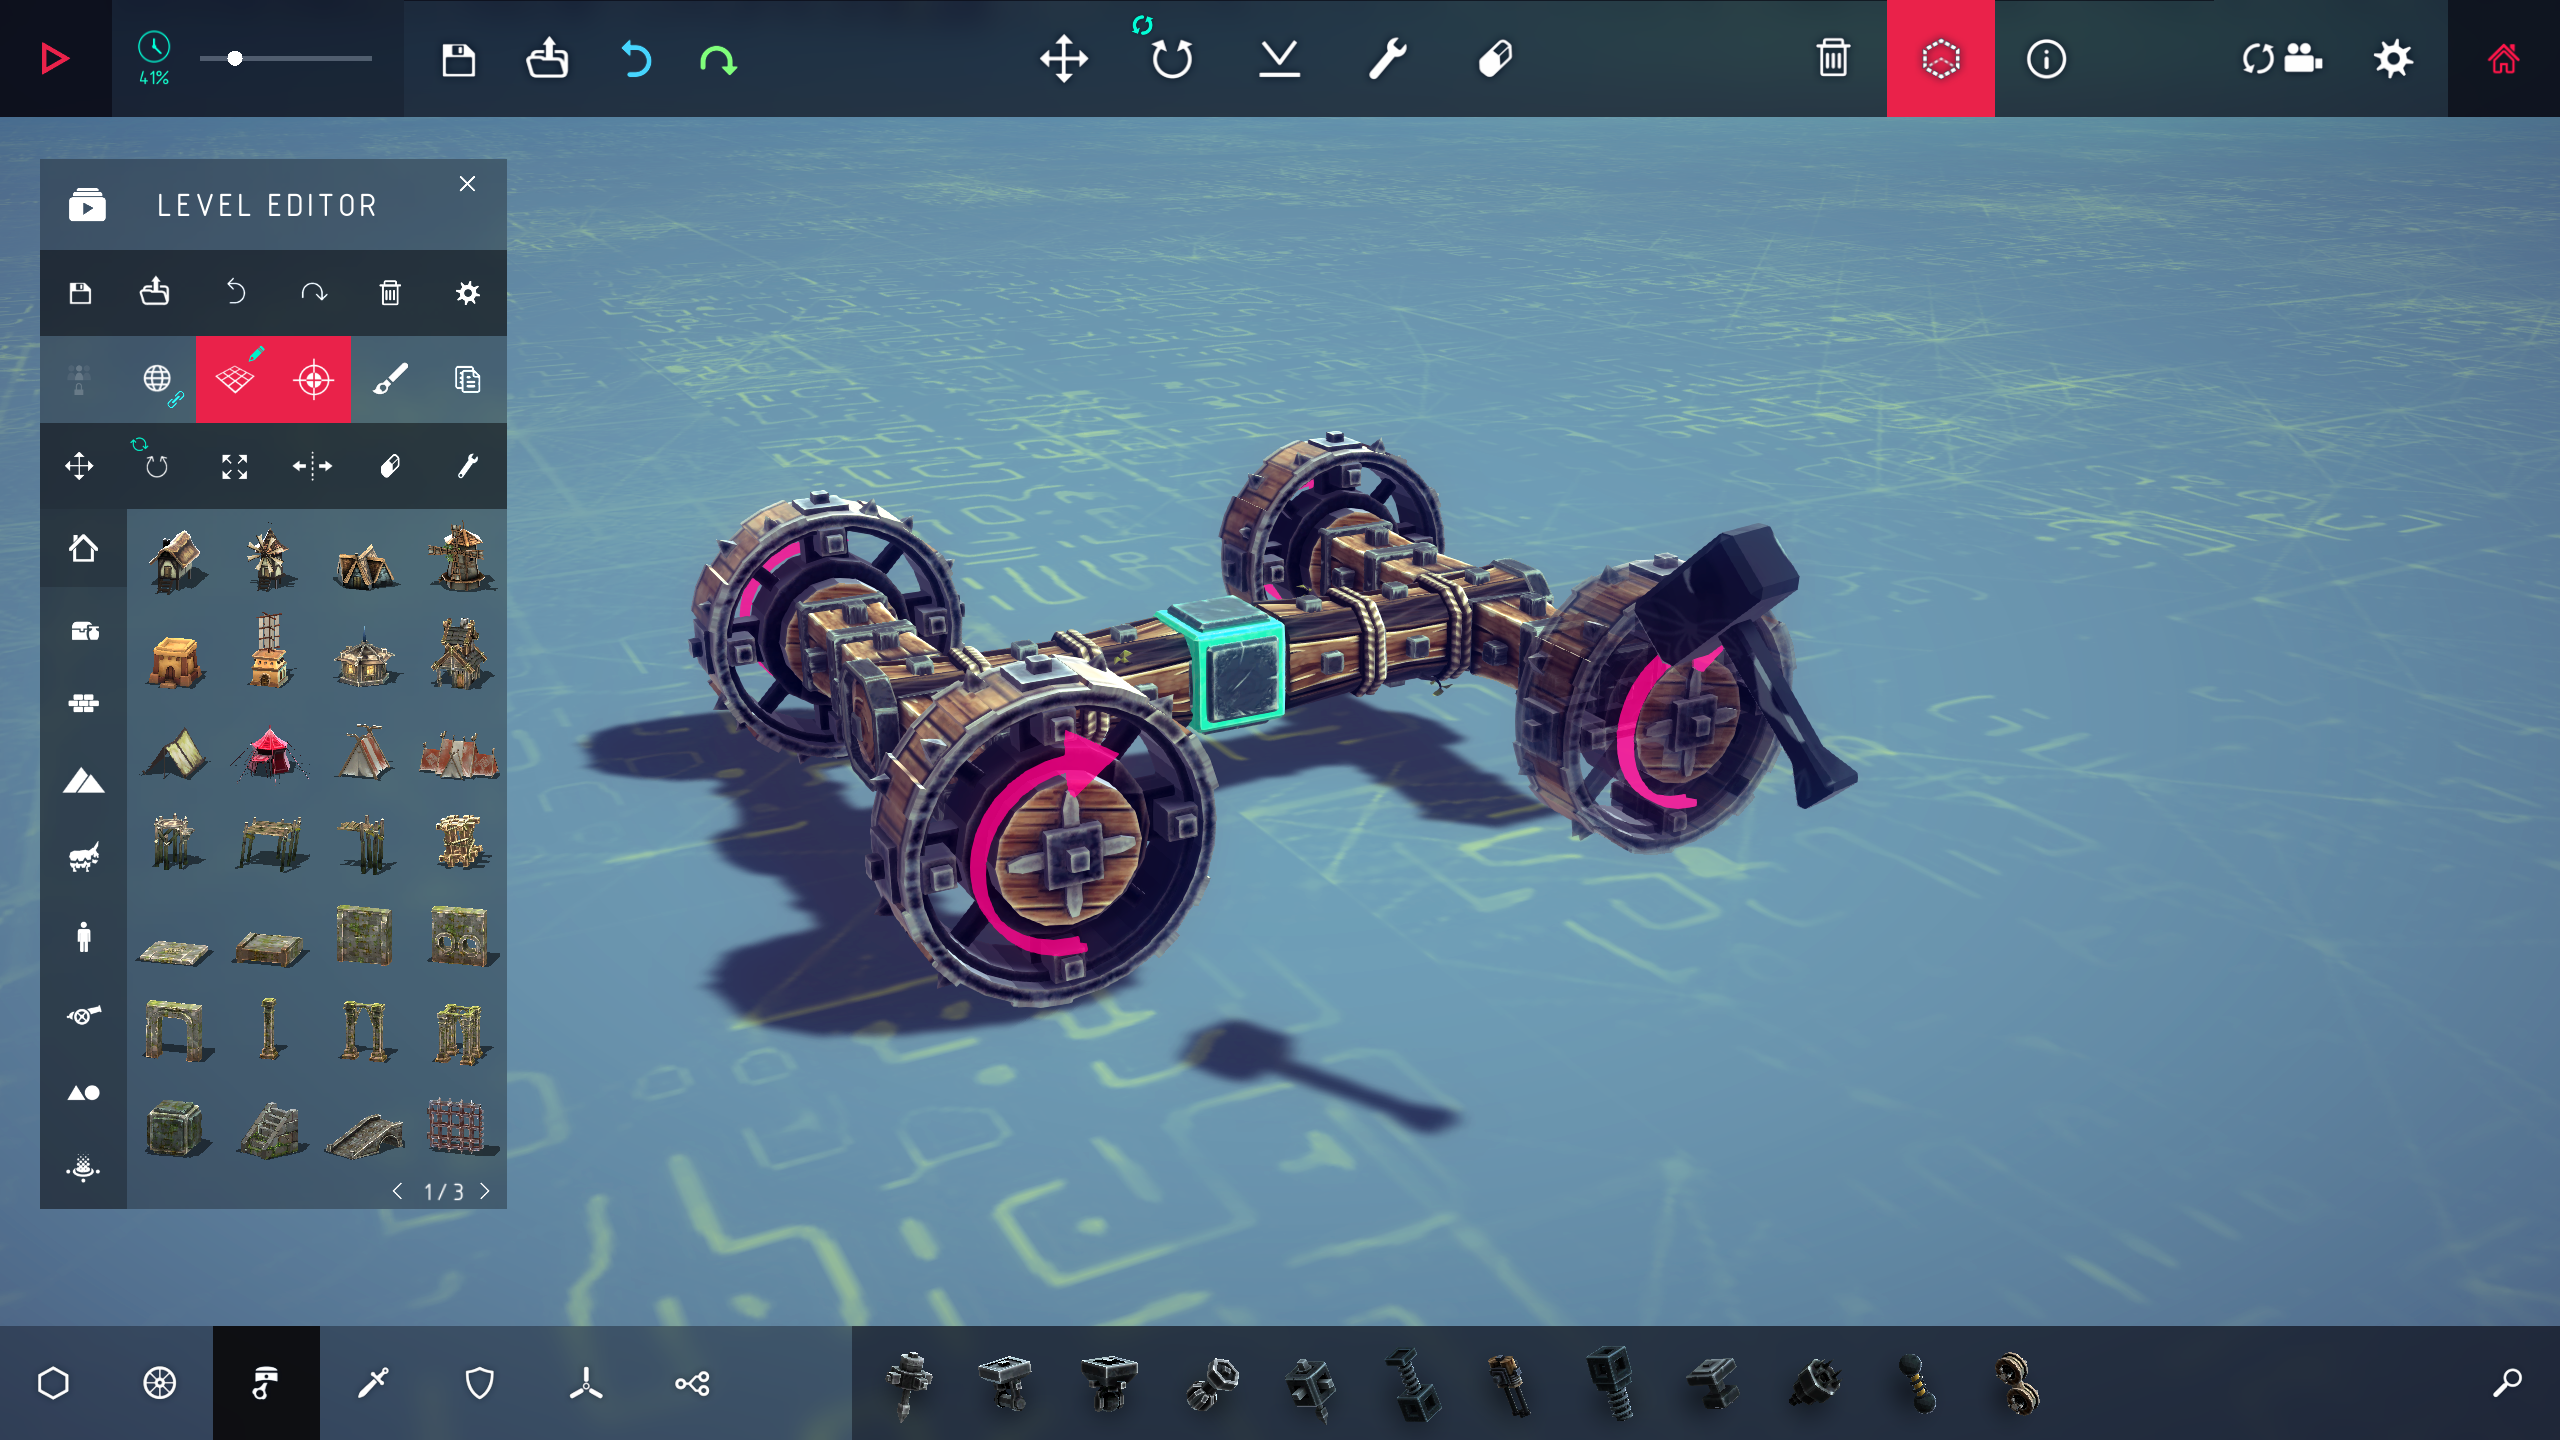
\includegraphics[width=0.9\linewidth]{figures/game_editor_view.png}
  \caption{\footnotesize Besiege editor view.}
  \label{fig:game_editor_view}
\end{figure}

\begin{figure}[h!]
  \centering
  \includegraphics[width=0.9\linewidth]{figures/block_stats.png}
  \caption{\footnotesize Common useful blocks in constructing standard machines in \envname.}
  \label{fig:block_intro}
\end{figure}

\subsection{Construction Rule}

Each machine is built by attaching new blocks to the existing structure, starting from a special root block. For convenience, we describe each construction step as an “attacher” block (child) connected to an “attachee” block (parent). As an attacher, each block has exactly one face available for connection; as an attachee, each block has none to several attachable faces. Once a face is used, it is considered occupied and cannot be reused. If, after construction, the free end of a block happens to coincide with an attachable face of an existing block, the two blocks are automatically connected.

A few special blocks violate the rule described above, such as spring. These blocks have two ends and thus must have two parent blocks, do not have physical volume can be attached to either vacant or occupied faces of other blocks.

Finally, each block can be rescaled and rotated after construction. Since post-construction scaling and rotation introduce unnecessary complexity into our pipeline, we exclude them from our experiments and leave their handling to future work.

\subsection{Simulation}

Once constructed, the machine will be placed at the designated pose indicated by the position and orientation of the starting block (not necessary near the ground, but there is a maximum height constraint). The machine will be subject to gravity and Newtonian physical laws (rigid and elastic ones) after placement.

\subsection{Blocks}\label{sec:b.1}
Out of the 75 construction blocks provided by Besiege, we filter out a list of 27 blocks (shown in Fig.~\ref{fig:block_intro}) that are most relevant to build machines with classical mechanical mechanisms such as levers and trusses.


\begin{itemize}
    \item \textbf{Starting Block}: the root of any mechanism; initial orientation is along z+ axis.
    \item \textbf{Small Wooden Block}: a cubic basic construction block.
    \item \textbf{Wooden Block}: shaped like two small wooden blocks attached together.
    \item \textbf{Wooden Rod}: a slender, fragile construction block.
    \item \textbf{Log}: shaped like three small wooden blocks arranged in parallel.
    \item \textbf{Steering Hinge}: powered; controls rotation of sub-blocks, swinging left or right along the axis perpendicular to its placement axis.
    \item \textbf{Steering Block}: powered; rotates blocks along its placement axis.
    \item \textbf{Powered Wheel}: radius 1m; provides ground movement.
    \item \textbf{Unpowered Wheel}: identical to the powered wheel but requires external force to rotate.
    \item \textbf{Large Powered Wheel}: larger version of the powered wheel (radius 3m).
    \item \textbf{Large Unpowered Wheel}: unpowered version of the large powered wheel.
    \item \textbf{Small Wheel}: functions like a caster wheel (e.g., shopping cart), unpowered, 1.2m long.
    \item \textbf{Roller Wheel}: similar to the small wheel, but shorter (0.8m).
    \item \textbf{Universal Joint}: freely rotates around its placement axis, unpowered.
    \item \textbf{Hinge}: swings up and down along the axis perpendicular to its placement axis, unpowered.
    \item \textbf{Ball Joint}: swings freely in all directions, unpowered.
    \item \textbf{Axle Connector}: similar to a ball joint but allows unrestricted $360^\circ$ rotation.
    \item \textbf{Suspension}: shaped like a wooden block, it can buffer
forces from all directions.
    \item \textbf{Rotating Block}: powered; motor-like block that generates torque and rotates about its local y-axis.
    \item \textbf{Grabber}: grabs objects on contact and can release them.
    \item \textbf{Boulder}: a large rock, loosely attached; useful for throwing.
    \item \textbf{Grip Pad}: block with the highest friction.
    \item \textbf{Elastic Pad}: block with the highest elasticity.
    \item \textbf{Container}: typically used to hold a boulder.
    \item \textbf{Spring}: can contract; one of the special blocks that can have two parent attachments (without occupying attachable faces).
    \item \textbf{Brace}: reinforces structural strength.
    \item \textbf{Ballast}: a heavy cubic block used as a counterweight.
\end{itemize}

\subsection{Tasks}

We define a set of tasks in which the goal is to construct machines within a designated building area to accomplish specific objectives.

\begin{itemize}
    \item \textbf{Movement.}
Referred to as the \textit{car} task in the main text, the objective is to build a machine capable of driving along tracks and traversing various terrains.
    \item \textbf{Throw.}
Referred to as the \textit{catapult} task in the main text, the goal is to construct a machine that can launch boulders over long distances. To prevent unintended strategies (e.g., carrying the boulder instead of throwing it, or letting it roll along the ground), the building area is enclosed by a medium-height wall.
    \item \textbf{Delivery.}
This task requires building a machine that can transport a large stone forward across different terrains (Fig.~\ref{fig:task_delivery}).

    \item \textbf{Pick.}
The objective here is to design a machine that can retrieve a stone located at the bottom of a deep well (Fig.~\ref{fig:task_pick}).

\end{itemize}

For many of these tasks, we introduce multiple difficulty levels (not used in the experiments reported in this paper) to encourage progressively more sophisticated designs:

\begin{itemize}
    \item \textbf{Movement and Delivery.}
We consider: (1) randomized terrains with stones and wooden rods (\eg, Fig.~\ref{fig:task_movement_rocky}), (2) curved tracks (Fig.~\ref{fig:task_curved_track}), and (3) obstacles such as height-limiting bars.

    \item \textbf{Throw.}
We design: (1) varied objectives, such as requiring the boulder to pass through an aerial ring (Fig.~\ref{fig:task_thru_ring}) or land precisely within a small target zone, (2) environmental factors such as wind, and (3) obstacles, including height restrictions either within the building area or along the boulder’s trajectory.

\end{itemize}


\begin{figure}[h!]
  \centering
  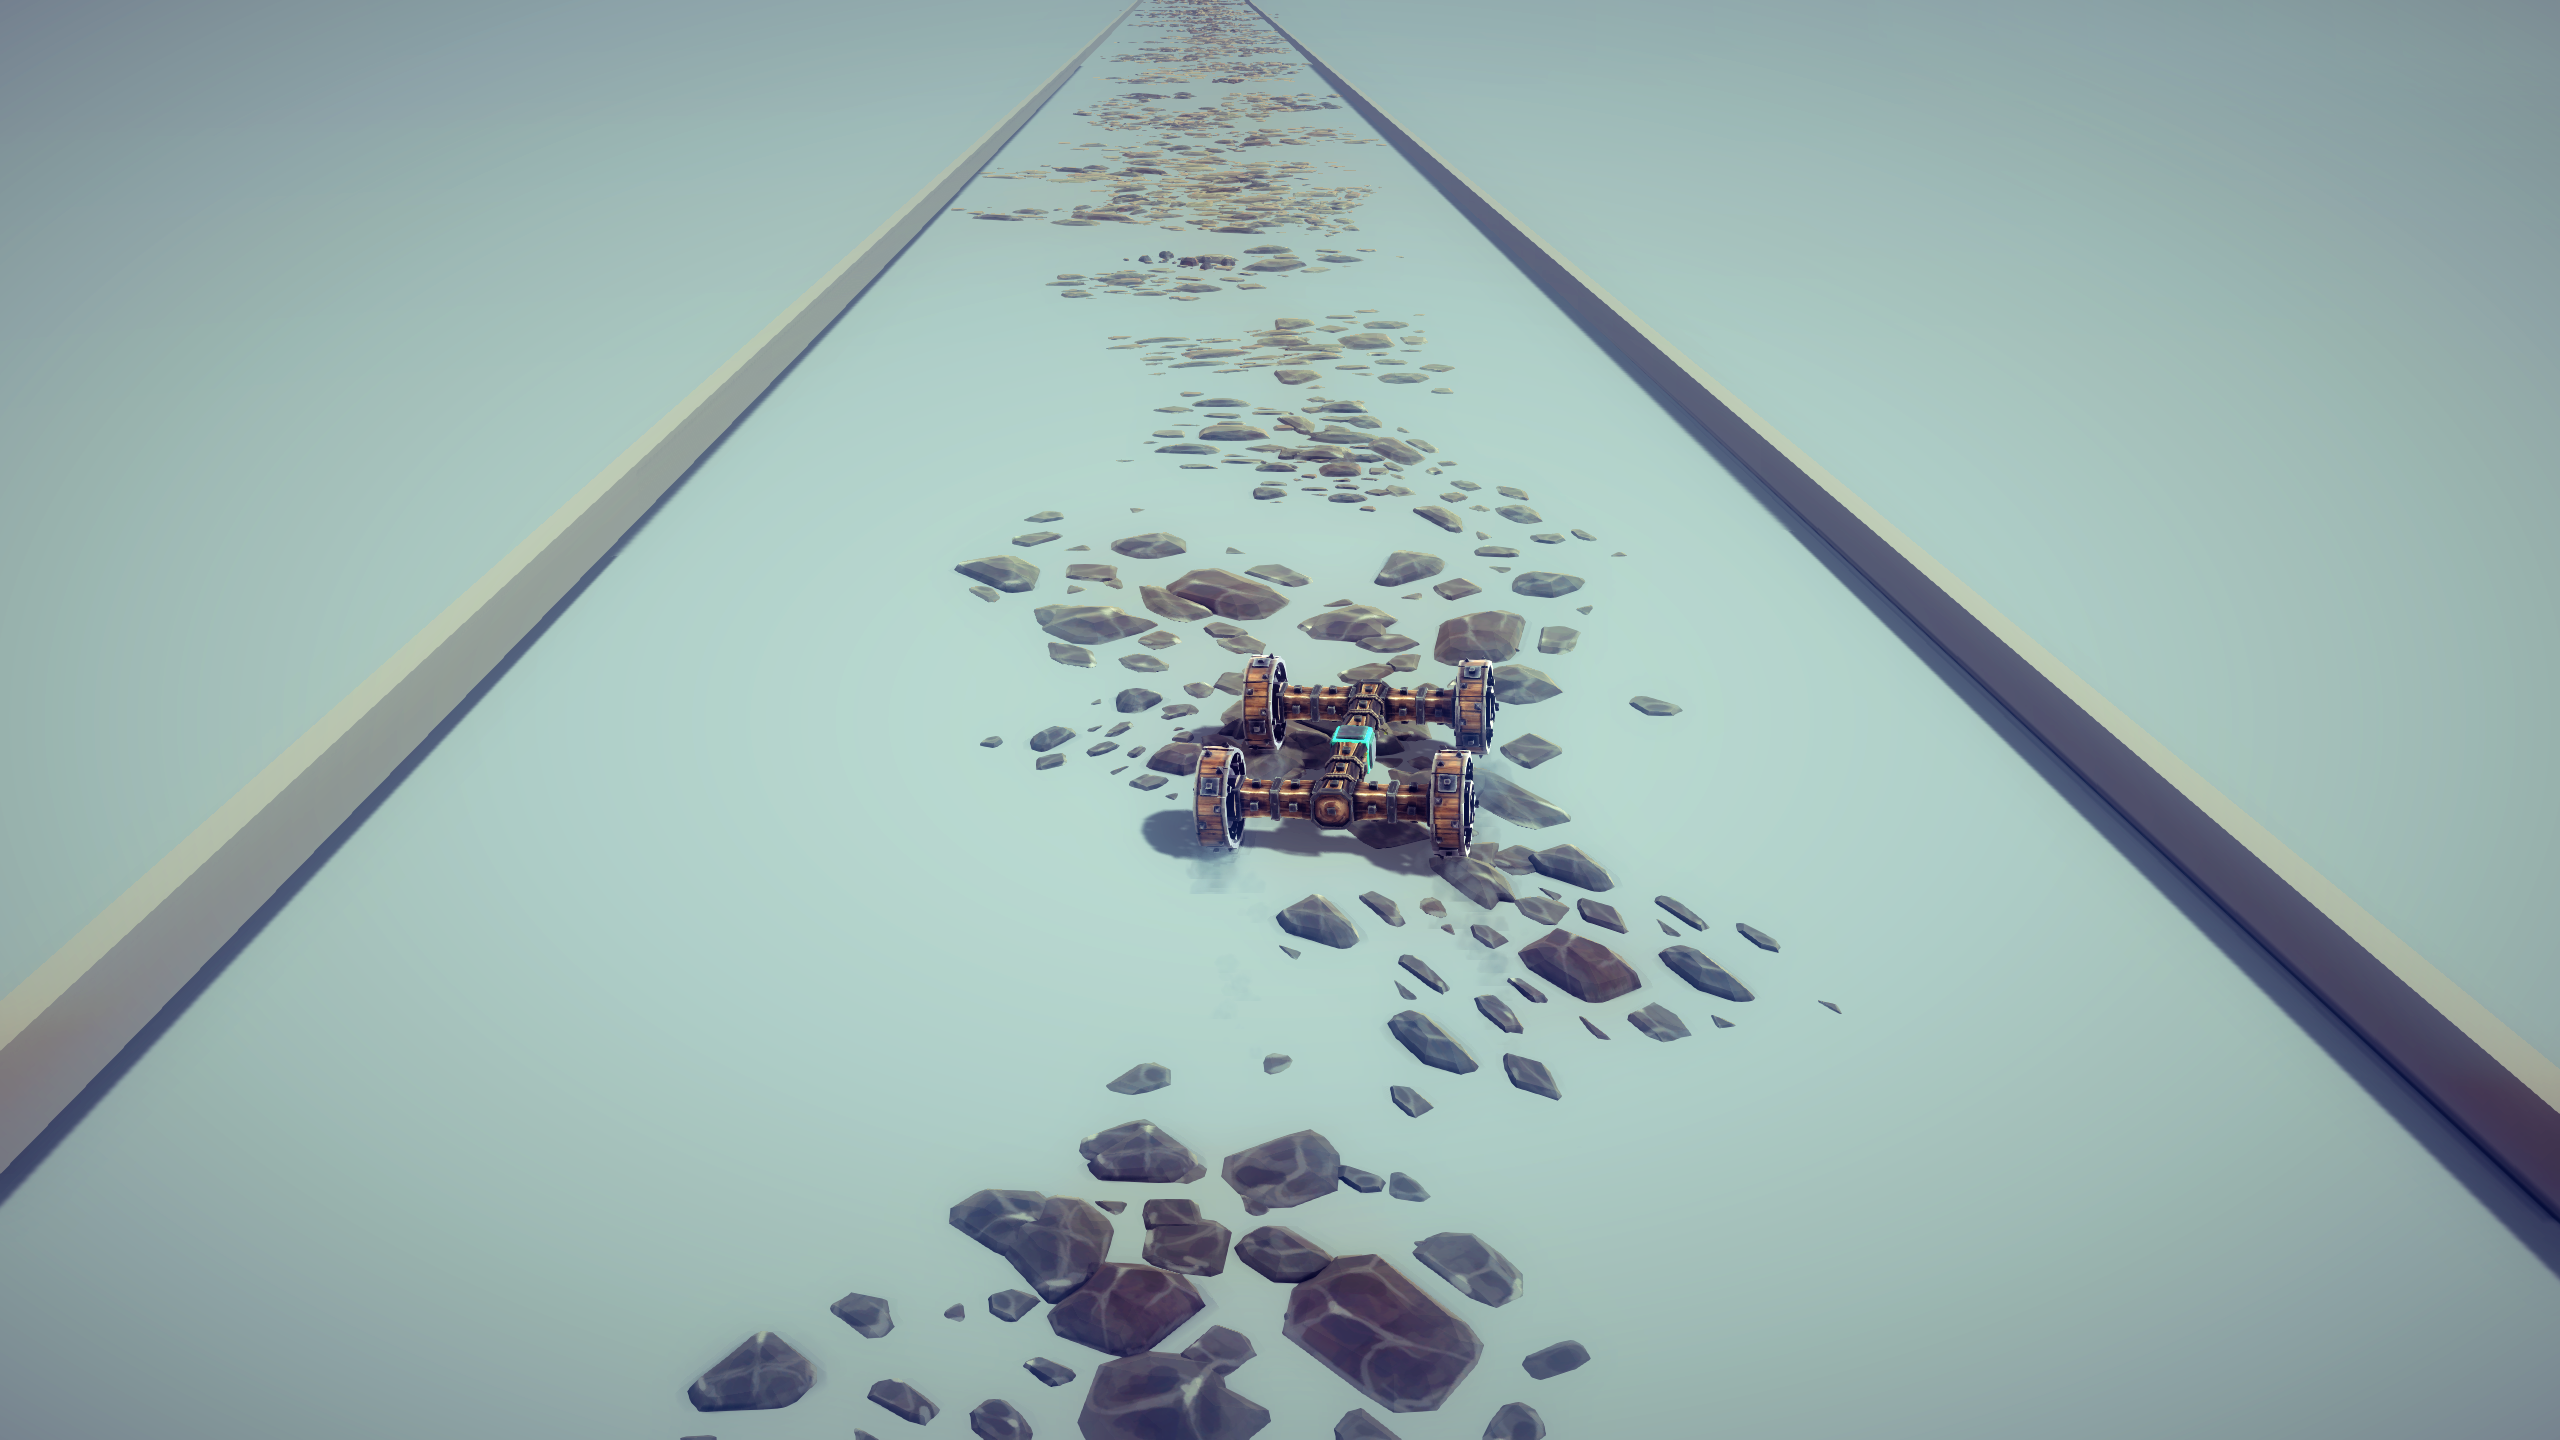
\includegraphics[width=\linewidth]{figures/tasks/movement_rocky.png}
  \caption{\footnotesize Illustration of the task \textit{car} / \textit{movement} on a rocky terrain, a more difficult setting compared to the environment used for the \textit{car} task in our experiments.}
  \label{fig:task_movement_rocky}
\end{figure}


\begin{figure}[h!]
  \centering
  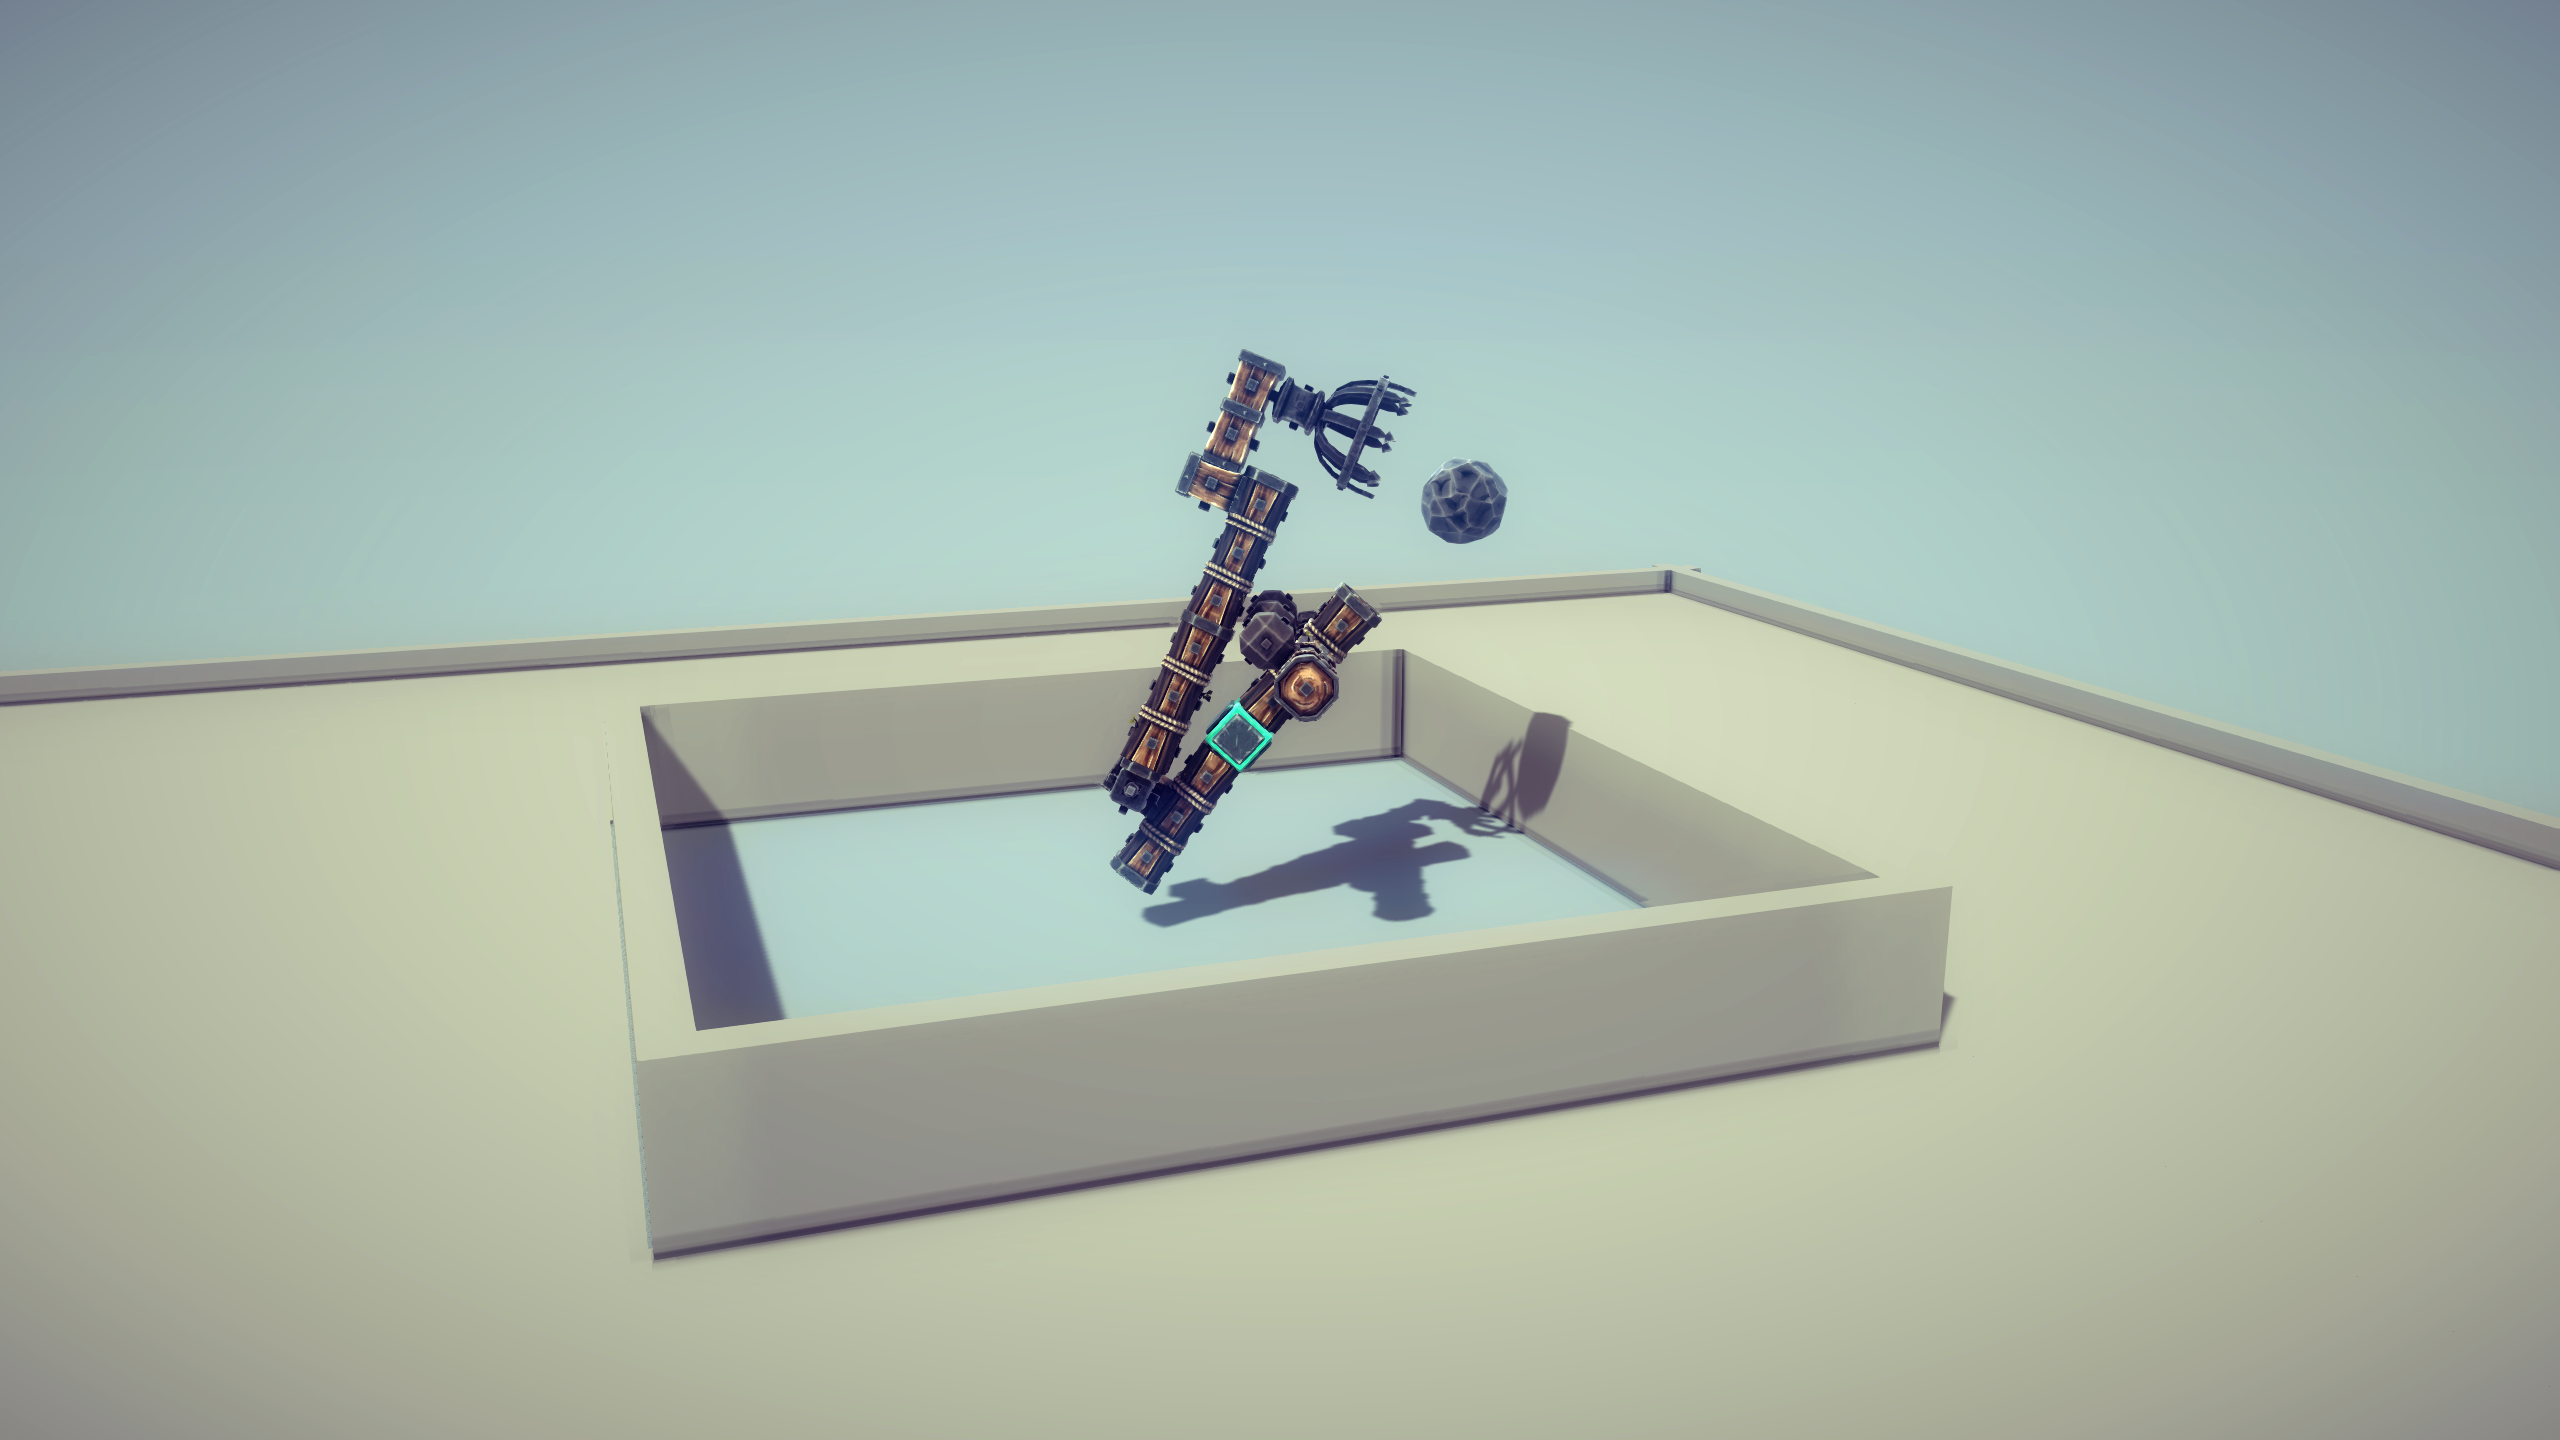
\includegraphics[width=\linewidth]{figures/tasks/throw.png}
  \caption{\footnotesize Illustration of the task \textit{catapult} / \textit{throw}.}
  \label{fig:task_throw}
\end{figure}


\begin{figure}[h!]
  \centering
  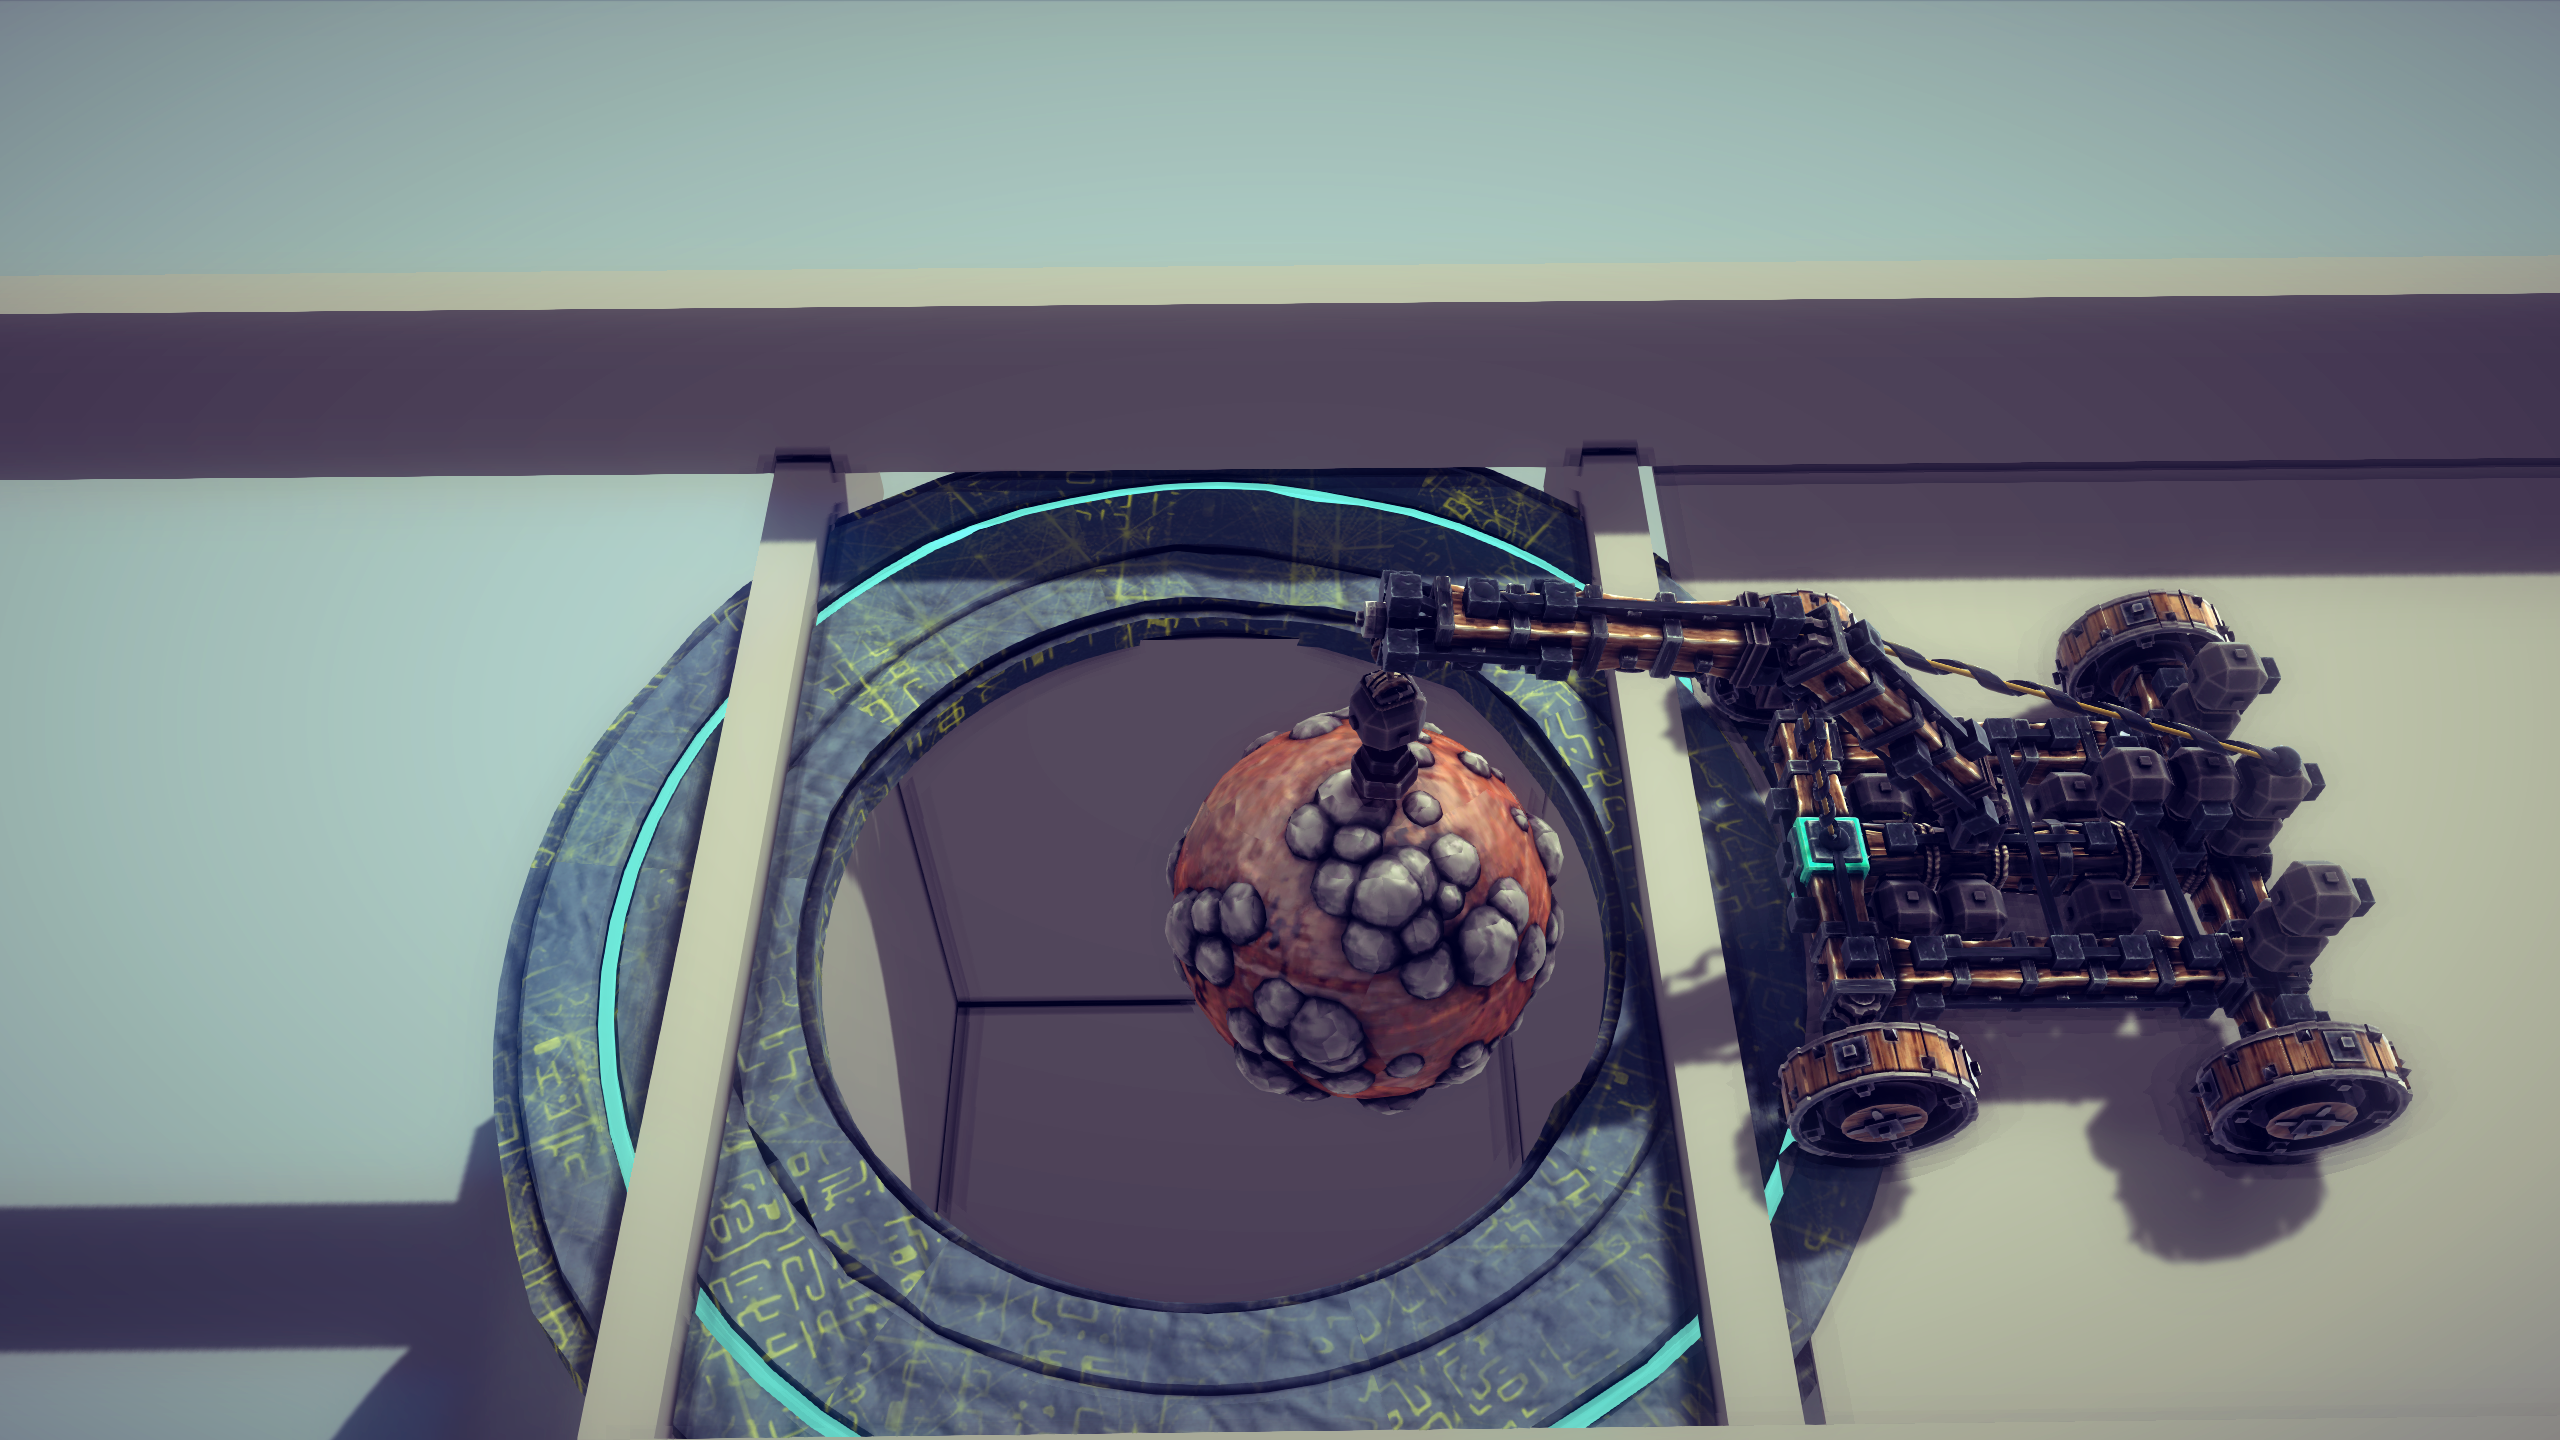
\includegraphics[width=\linewidth]{figures/tasks/pick.png}
  \caption{\footnotesize Illustration of the task \textit{pick}.}
  \label{fig:task_pick}
\end{figure}


\begin{figure}[h!]
  \centering
  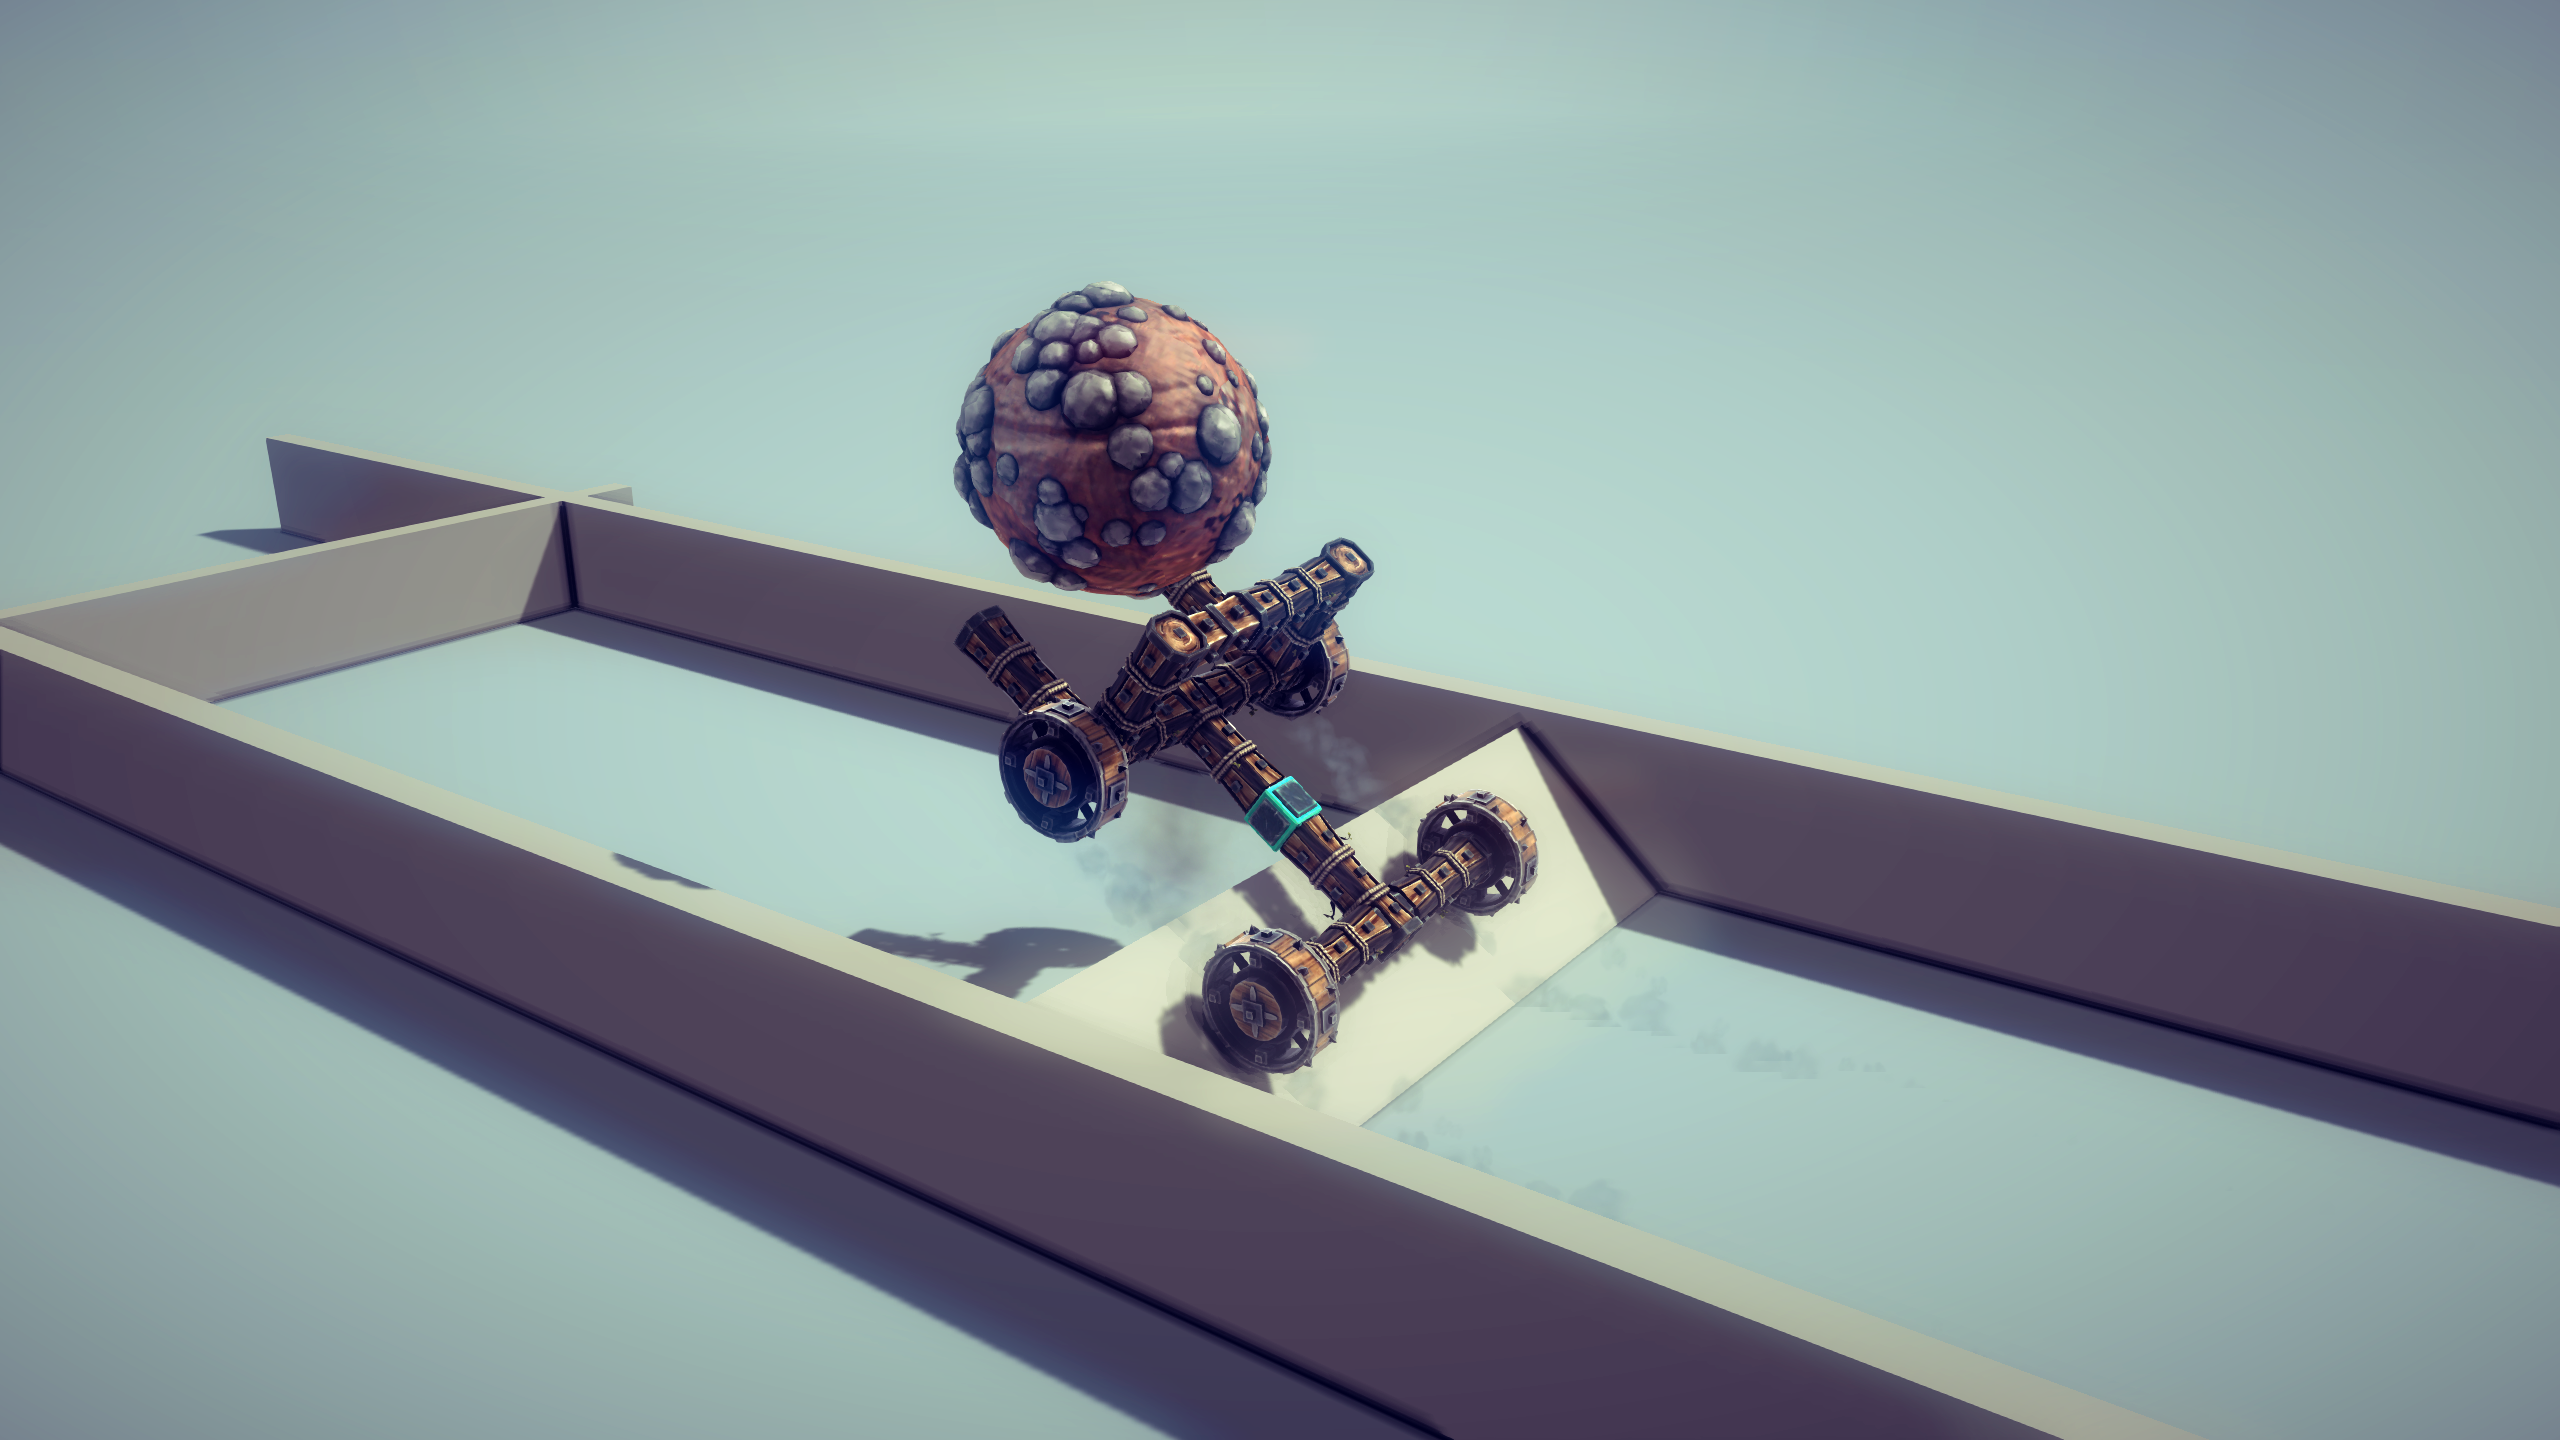
\includegraphics[width=\linewidth]{figures/tasks/delivery.png}
  \caption{\footnotesize Illustration of the task \textit{delivery} with a bump on the track.}
  \label{fig:task_delivery}
\end{figure}


\begin{figure}[h!]
  \centering
  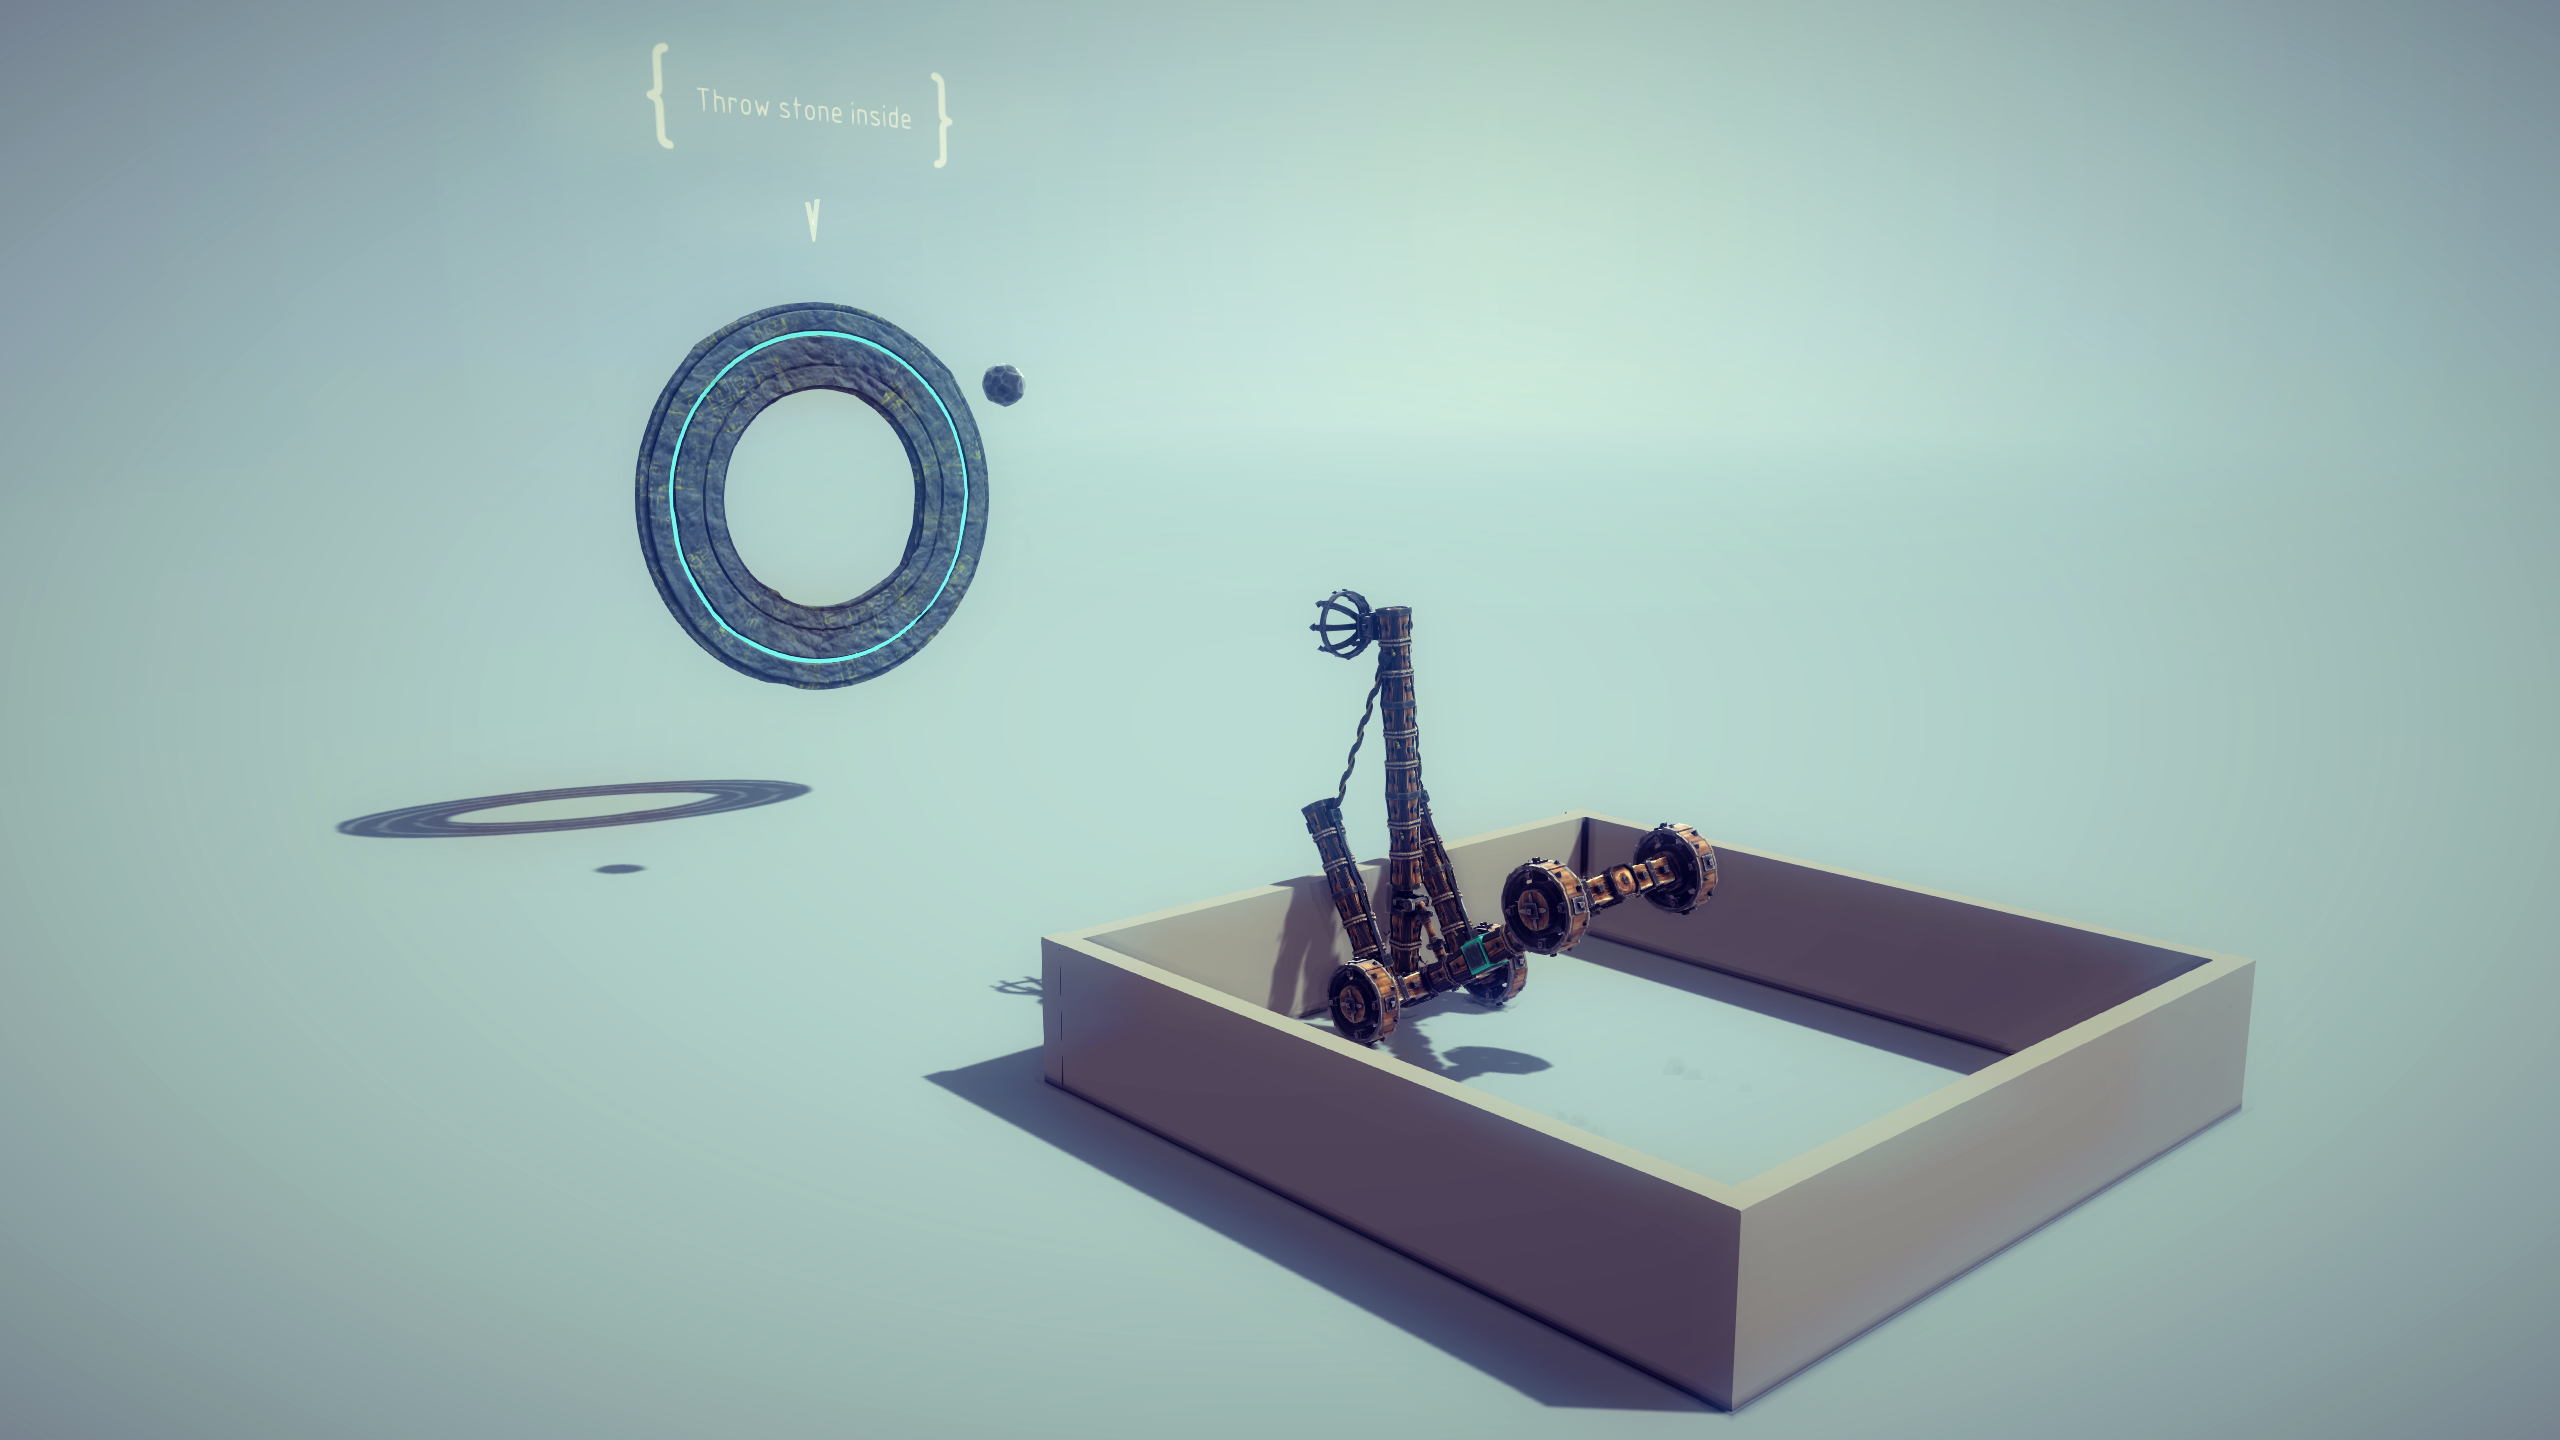
\includegraphics[width=\linewidth]{figures/tasks/thru_ring.png}
  \caption{\footnotesize Illustration of the task \textit{catapult} / \textit{Throw} with the objective of throwing the boulder through the target ring.}
  \label{fig:task_thru_ring}
\end{figure}


\begin{figure}[h!]
  \centering
  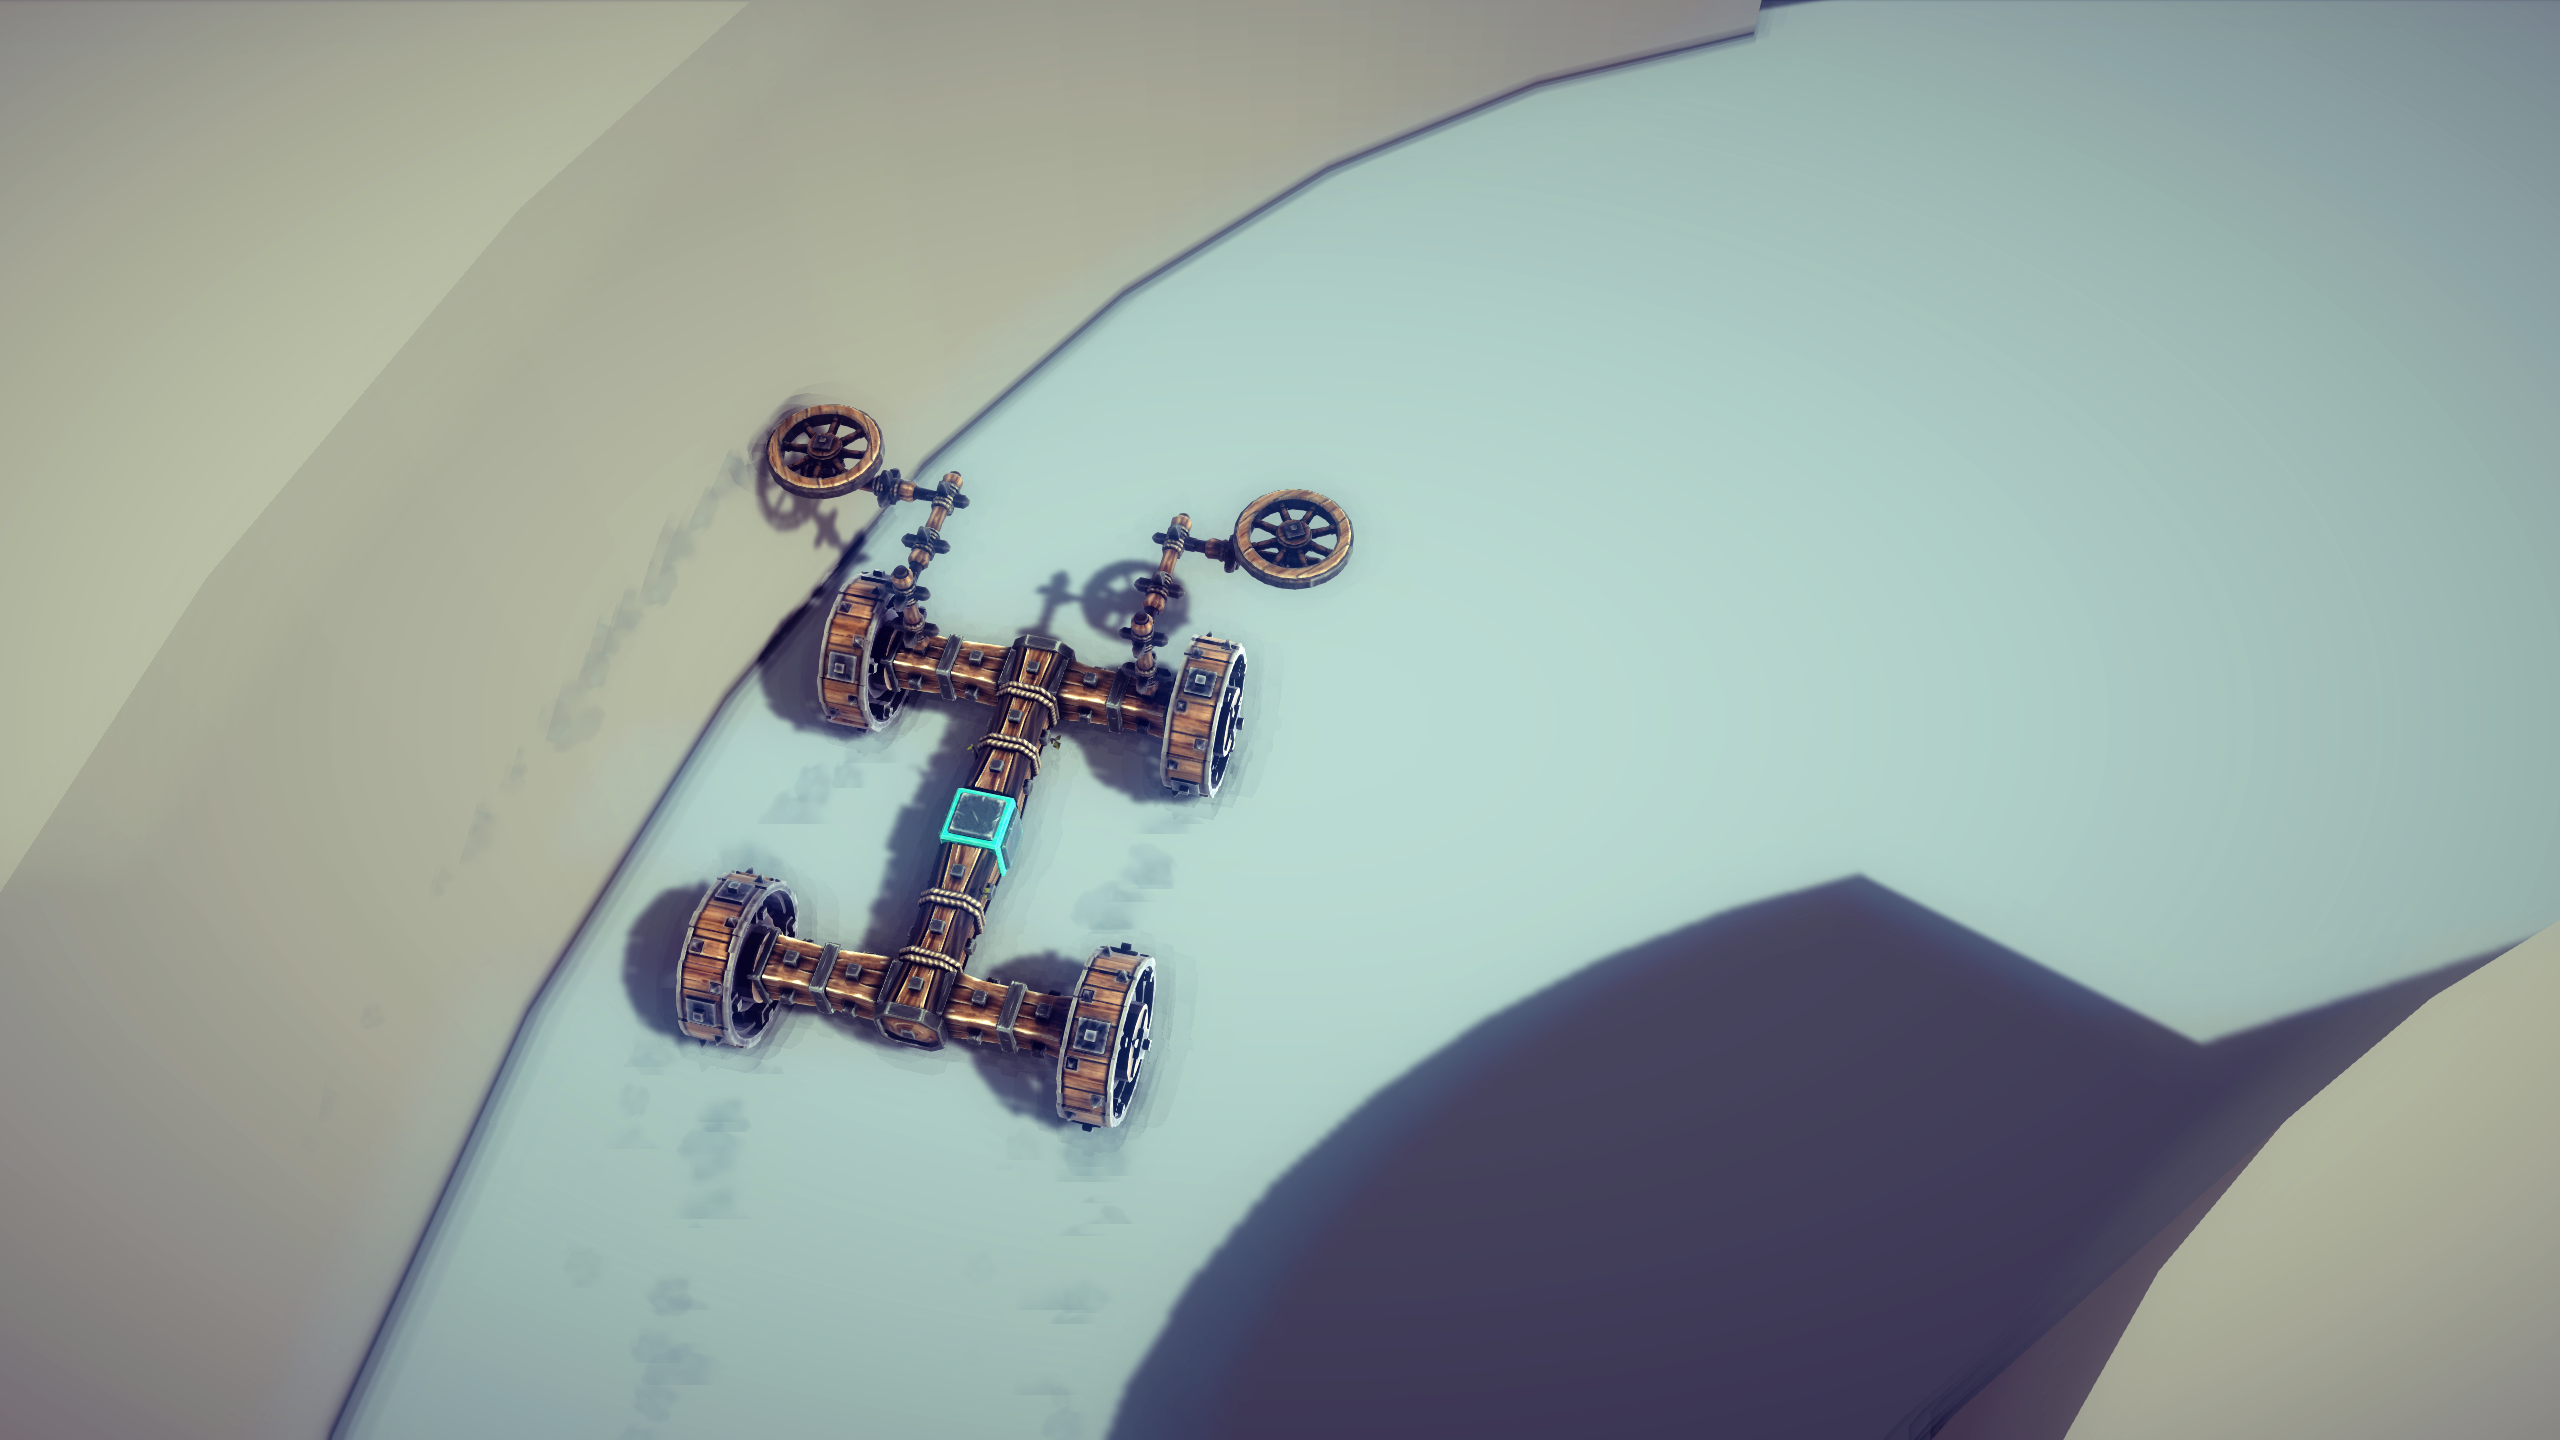
\includegraphics[width=\linewidth]{figures/tasks/curved_track.png}
  \caption{\footnotesize Illustration of the task \textit{car} / \textit{movement} with a curved track.}
  \label{fig:task_curved_track}
\end{figure}











\clearpage
\newpage

\section{Search Strategies in Machine Modification Loops}



Apart from the MCTS strategy used in the main experiments, we also evaluate two alternatives: (i) best-of-N, where we select the best-performing machine out of N candidates, and (ii) random search, which mimics best-of-N but instead selects a random candidate. For clarity, we refer to one consecutive ``querier–refiner'' call as a search node (consistent with our MCTS setup). Unlike classical MCTS or best-of-N, here each search node is allowed up to five retries to prevent child statistics from being too sparse. We perform $R$ search rounds, each aiming to obtain $5$ valid candidate machines (though this may fail; if fewer than 5 are found, the parent node’s machine is used as a candidate). Full algorithmic details are provided in Algorithm~\ref{alg:random-search}, Algorithm~\ref{alg:bestofn}, and Algorithm~\ref{alg:mcts}. In Fig.~\ref{tab:mcts_ablation} we show the improvement of machine performance with respect to the number of search rounds used. In Fig.~\ref{fig:search_curve} we compare the efficiency of different search methods in our agentic compositional machine design setting.



\begin{algorithm}
\caption{Random Search Algorithm}
\label{alg:random-search}
\begin{algorithmic}[1]
\Require Agentic Search Node $N$
\Require Scoring function $S$, machine valid check function $F$
\Require Search Round $R$
\Ensure The Best result with the highest score

\State Input machine $ori\_machine$
\State $max\_retry \gets 5$
\State $machine\_last\_round \gets ori\_machine$

\For{$r=1$ to $R$}
    \State $best\_score \gets -\infty$
    \State $retry \gets 0$
    \While{$retry < max\_retry$}
        \State $retry \gets retry + 1$
        \State $machine\_next\_round \gets N.generate(machine\_last\_round)$
        \If{$F(machine\_next\_round)$}
            \State \textbf{break} 
        \EndIf
    \EndWhile
    \State $score \gets S(machine\_next\_round)$
    \State $machine\_last\_round \gets machine\_next\_round$
\EndFor

\State \Return $(machine\_last\_round, score)$
\end{algorithmic}
\end{algorithm}


\begin{algorithm}
\caption{Best-of-N Algorithm}
\label{alg:bestofn}
\begin{algorithmic}[1]
\Require Agentic Search Node $N$
\Require Scoring function $S$, machine valid check function $F$
\Require Search Round $R$, number of samples $n$
\Ensure The Best result with the highest score

\State Input machine $ori\_machine$
\State $best\_score \gets -\infty$
\State $best\_machine \gets ori\_machine$
\State $max\_retry \gets 5$

\For{$r=1$ to $R$}
    \State $best\_score \gets -\infty$
    \State $best\_machine\_this\_round \gets best\_machine$
    \For{$i=1$ to $n$}
        \State $retry \gets 0$
        \While{$retry < max\_retry$}
            \State $retry \gets retry + 1$
            \State $machine_i \gets N.generate(best\_machine\_this\_round)$
            \If{$F(machine_i)$}
                \State \textbf{break} 
            \EndIf
        \EndWhile
        \State $score_i \gets S(machine_i)$
        \If{$score_i > best\_score$}
            \State $best\_score \gets score_i$
            \State $best\_machine \gets machine_i$
        \EndIf
    \EndFor
\EndFor

\State \Return $(best\_machine, best\_score)$
\end{algorithmic}
\end{algorithm}


\begin{algorithm}
\caption{Monte Carlo Tree Search (MCTS)}
\label{alg:mcts}
\begin{algorithmic}[1]
\Require Agentic Search Node $N$
\Require Root node $root$, maximum iterations $MAX\_ITER$
\Require \text{Select}(node): Traverse tree using UCB until leaf node
\Require \text{Expand}(node): Generate 4 child candidates via LLM. Validate them in parallel: keep valid ones, and regenerate invalid ones until they pass or hit the max retry limit. If all fail, use the parent node as the child.
\Require \text{Simulate}(node): Besiege simulation
\Require \text{Backpropagate}(node, reward): Update visit counts and rewards along path
\Require \text{BestChild}(node): Return child with highest simulation score
\Ensure Best action from the search tree

\State $root \gets s_0$
\State $max\_retry \gets 5$
\For{$i = 1$ to $MAX\_ITER$}
    \State $retry \gets 0$
    \State $node \gets \text{Select}(root)$ \Comment{Step 1: Selection}
    \If{$\textit{node} == \textit{root}$ or $\textit{node}.\textit{visited}$}
        \State $\textit{should\_expand} \gets True$
    \EndIf
    \If{not $\textit{should\_expand}$}
        \State $child \gets node$ \Comment{Unvisited leaf \textit{node}; no children yet}
    \EndIf
    \While{$\textit{should\_expand}$ and not all child nodes are valid}
        \State $retry \gets retry + 1$
        \State $child \gets \text{Expand}(node)$ \Comment{Step 2: Expansion}
        \If{$retry \geq max\_retry$}
            \State \textbf{break} 
        \EndIf
    \EndWhile
    \State $reward \gets \text{Simulate}(child)$ \Comment{Step 3: Simulation}
    \State $\text{Backpropagate}(child, reward)$ \Comment{Step 4: Backpropagation}
\EndFor
\State \textbf{return} $\text{BestChild}(root)$ \Comment{Return best child}
\end{algorithmic}
\end{algorithm}



\begin{table}[h!]
  \centering
  \setlength{\tabcolsep}{6pt}       %
  \renewcommand{\arraystretch}{1.2} %
  \newcommand{\cgr}[1]{\textcolor[rgb]{.329, .51, .208}{\textbf{#1}}}
  \newcommand{\cre}[1]{\textcolor[rgb]{1, 0, 0}{\textbf{#1}}}
  \begin{tabularx}{\textwidth}{l*{9}{>{\centering\arraybackslash}X}} %
    \toprule
    \multirow{2}{*}{Models} & \multicolumn{3}{c}{Random Search} & \multicolumn{3}{c}{Best-of-N } & \multicolumn{3}{c}{MCTS} \\
    \cmidrule(lr){2-4} \cmidrule(lr){5-7} \cmidrule(lr){8-10}
     & Avg.I & Mean  & Max & Avg.I & Mean  & Max & Avg.I & Mean  & Max \\
    \midrule
    Gemini 2.5 Pro       & 5 & 15.02     & 20.5    & 20 & 14.67  &16.66  & 8 &15.73     & 18.19     \\
    Claude Opus 4       & 5 &  7.67   &  7.88   & 18 & 8.18  & 8.50  & 6 &  9.10    &   9.32   \\
    o3                    & 5 & 7.71     & 11.94     & 8 & 10.60  &15.07  & 7 & 5.34     & 11.11     \\
    Qwen3-Coder-480B-A35B & 5 &4.50     &7.64     & 11 &5.61   &9.87  & 8.5 & 5.21  & 6.52  \\
    \bottomrule
  \end{tabularx}
  \caption{\footnotesize Ablation study on different search strategies. We compare the agentic workflow final scores. MCTS is executed for 5 rounds, with Random Search and Best-of-N also run for the same number of rounds. Avg.I denotes the average number of node expansions per search round.}
  \label{tab:abl:env-search}
\end{table}


\begin{table}[h!]
  \centering
  \setlength{\tabcolsep}{6pt}       %
  \renewcommand{\arraystretch}{1.2} %
  \newcommand{\cgr}[1]{\textcolor[rgb]{.329, .51, .208}{\textbf{#1}}}
  \newcommand{\cre}[1]{\textcolor[rgb]{1, 0, 0}{\textbf{#1}}}
  \begin{tabularx}{\textwidth}{l*{6}{>{\centering\arraybackslash}X}} %
    \toprule
    \multirow{2}{*}{Models} & \multicolumn{2}{c}{R2} & \multicolumn{2}{c}{R5} & \multicolumn{2}{c}{R10} \\
    \cmidrule(lr){2-3} \cmidrule(lr){4-5} \cmidrule(lr){6-7}
     & Mean  & \multicolumn{1}{c}{Max} & Mean  & \multicolumn{1}{c}{Max} & Mean  & Max \\
    \midrule
    Gemini 2.5 Pro            &15.04&17.31&15.73&18.19&16.44&18.19\\
    Claude Opus 4       &8.61&9.32&9.10&9.32&9.43&9.98\\
    o3                   &5.33&11.11&5.34&11.11&8.46&14.52 \\
    Qwen3-Coder-480B-A35B &5.18&6.52&5.21&6.52&5.74&6.52\\
    \bottomrule
  \end{tabularx}
  \caption{\footnotesize Ablation study on the effect of search depth in MCTS. R2, R5, and R10 represent the running rounds of MCTS on the same search tree.}
  \label{tab:mcts_ablation}
\end{table}

\begin{figure}[h!]
  \centering
  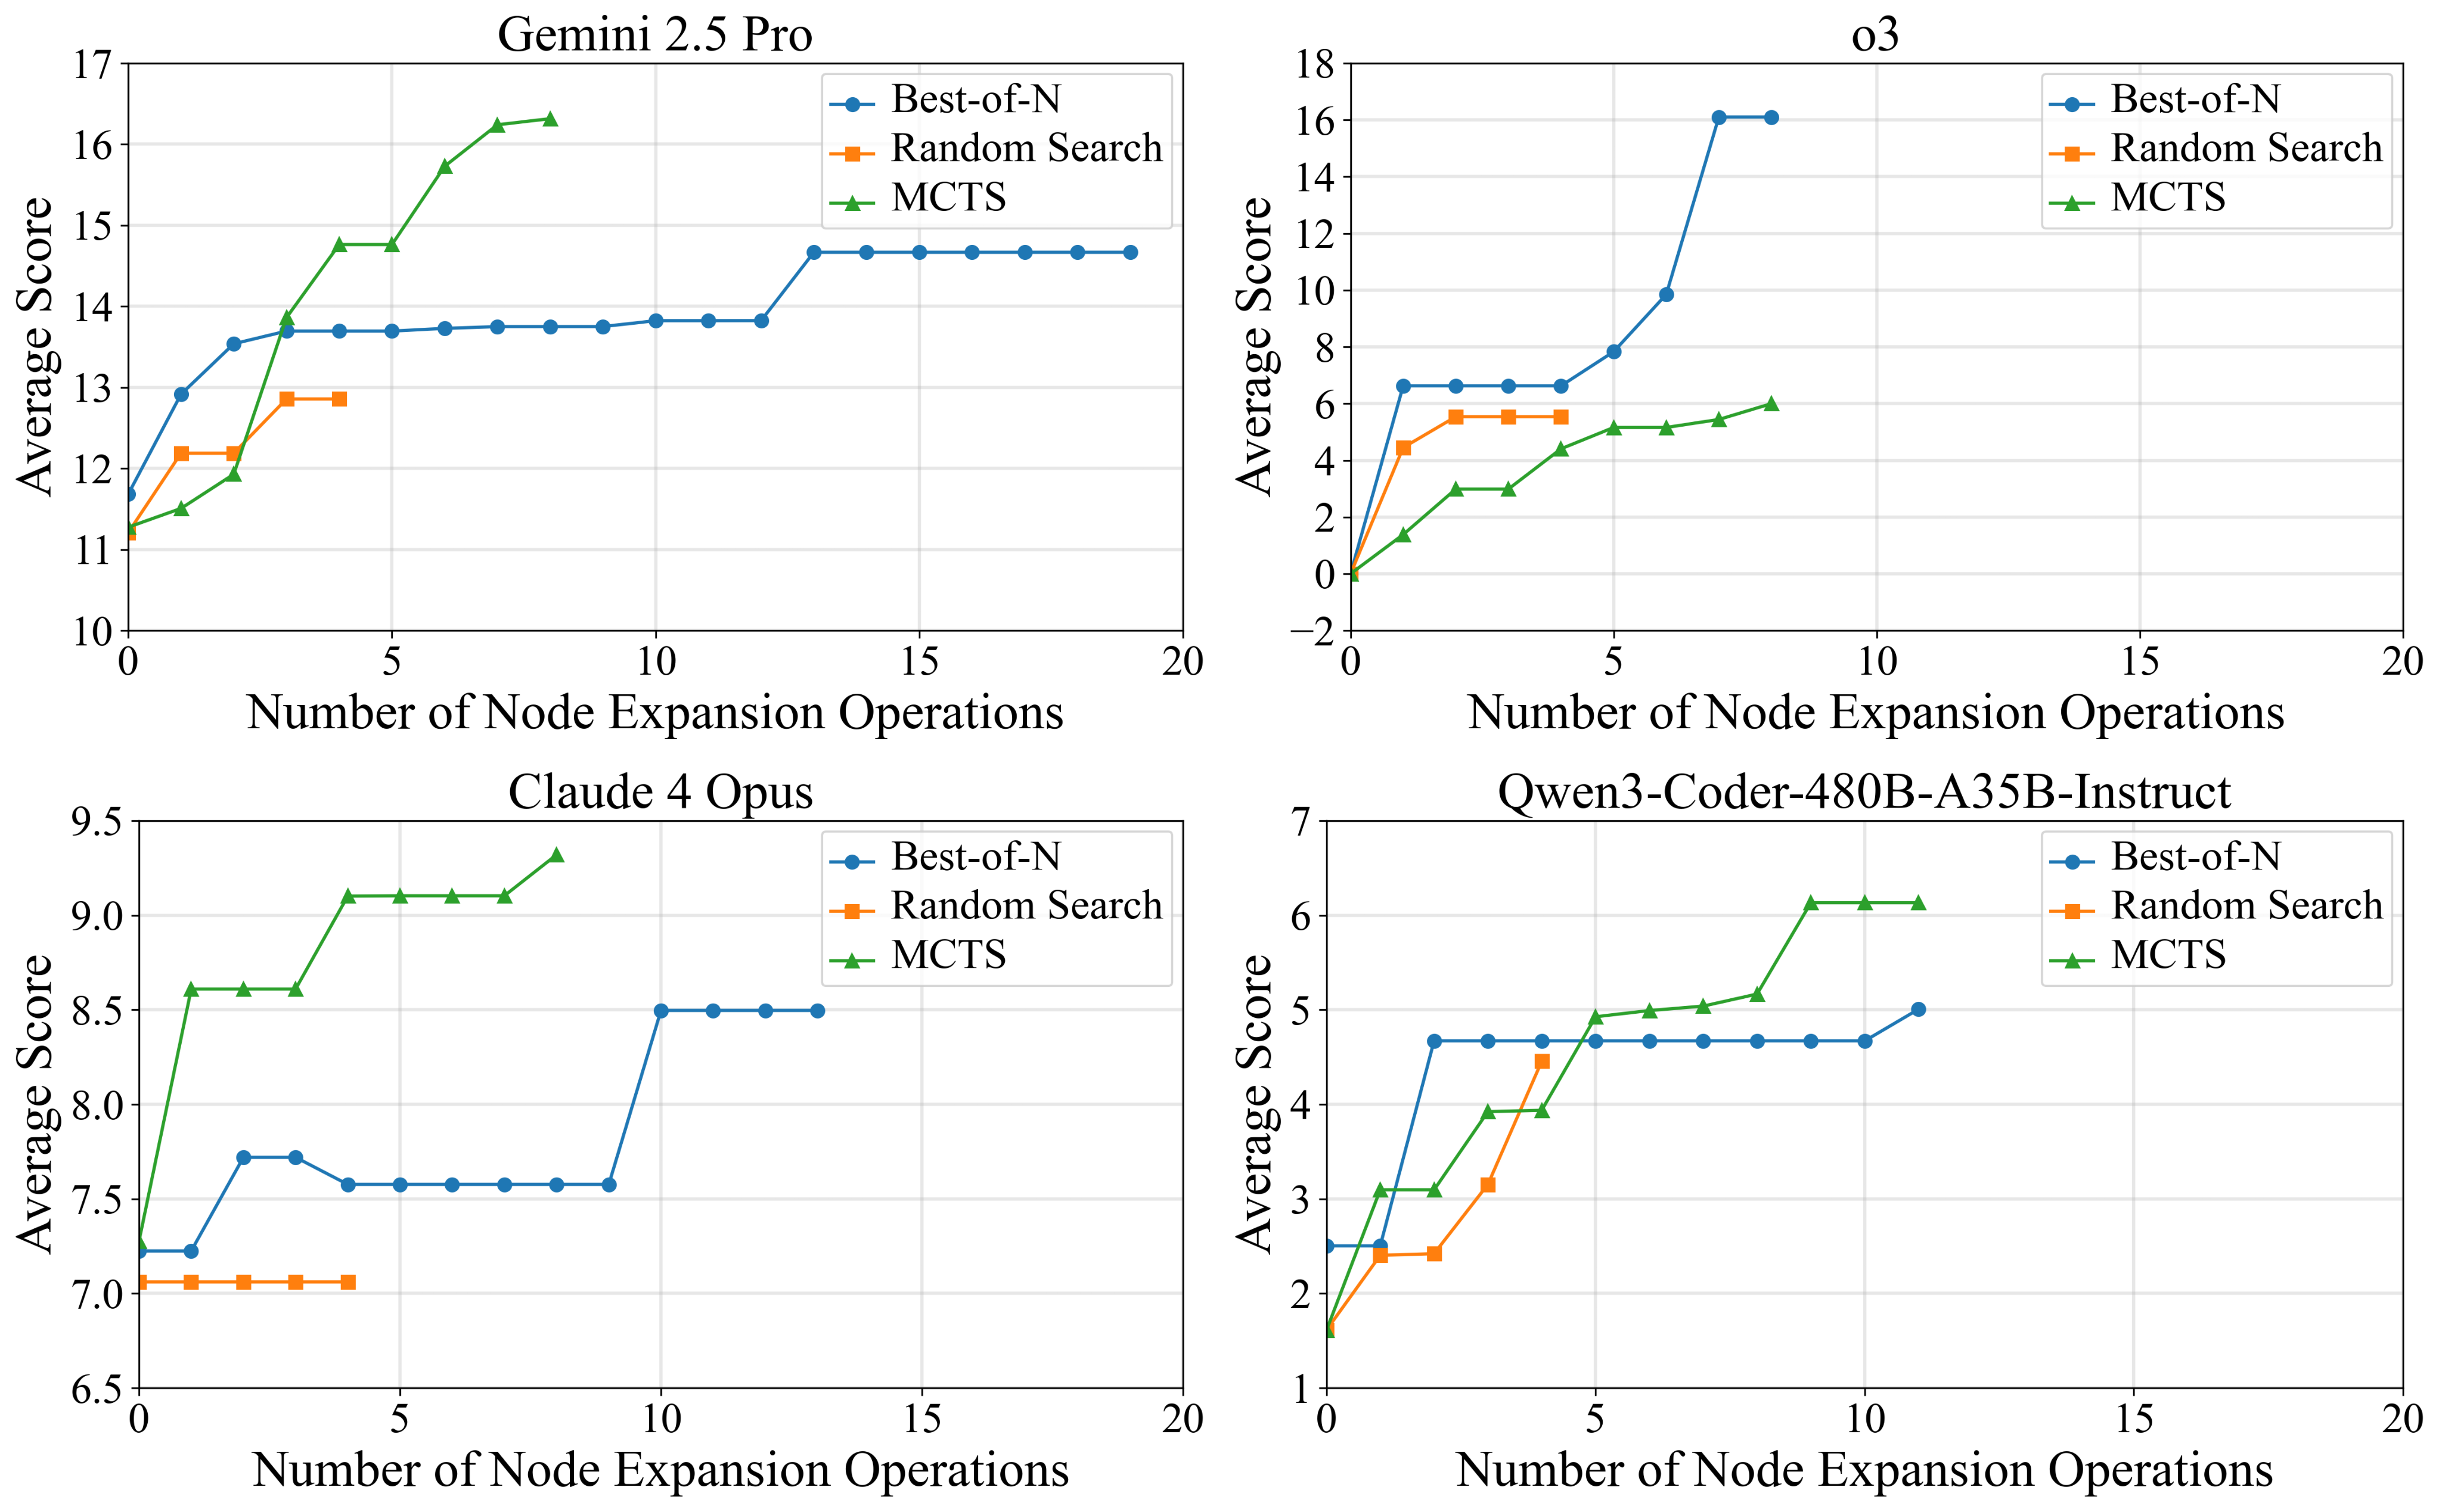
\includegraphics[width=\linewidth]{figures/RL_Metrics/search_strategy.png}
  \caption{\footnotesize The variation in machine average scores with the increasing number of LLM node expansion operations under different search strategies.}
  \label{fig:search_curve}
\end{figure}

\clearpage
\newpage
\section{Environment Settings for Agentic Design and RL Finetuning}

\subsection{Machine Representation}
\label{sec:machine_rep}

To reduce complexity in compositional machine design, our machine representation assumes all blocks remain at their default scale and are not further rotated after attachment (note: the attachment operation itself may rotate blocks).

\subsection{Global Position-based Representation}
By simplifying the default XML representation that \envname receives, we obtain the global position-based representation. Below is a concrete example:
\begin{lstlisting}
[
    {"type": 0, "Position": [0,0,  0], "Rotation": [0,0,0,1]},
    {"type": 1, "Position": [0,0,0.5], "Rotation": [0,0,0,1]},
    {"type": 2, "Position": [0,0,2.5], "Rotation": [0,0,0,1]},
    {"type": 9, "Position": [0,0.5,2], "Rotation": [-0.707,0,0,0.707],
                "end-position": [0,2,0]}
]
\end{lstlisting}

Basically, each block in the machine is independently recorded without mentioning its adjacent blocks. For most of the block types, only the block type and its pose (position + orientation) are recorded. For special blocks that have two parents, the other end has to be specified, for which the corresponding dictionary has an additional entry of ``end-position''.


\subsection{Construction Tree Representation}
\label{sec:tree_rep}

With our parsimonious construction tree representation, the example machine above is represented by the following the following JSON list:
\begin{lstlisting}
[
    {'type': 0, 'id': 0, 'parent'  : -1, 'face_id'  : -1}, 
    {'type': 1, 'id': 1, 'parent'  :  0, 'face_id'  :  0}, 
    {'type': 2, 'id': 2, 'parent'  :  1, 'face_id'  :  0}, 
    {'type': 9, 'id': 3, 'parent_a':  0, 'face_id_a':  4,
                         'parent_b':  1, 'face_id_b':  6}
]
\end{lstlisting}

Specifically, the ordered list of dictionaries of the machine construction JSON file represents the construction order of blocks. Each dictionary contains the following information of corresponding block: 1) ``type'': block type; 2) ``id'': the order ID of this block (the same as the order in the list), included so that LLMs do not have to parse it by itself; 3) ``parent'', the ID of its parent block; 4) ``face\_id'', the face of the block's parent to which the block is attached. In cases that the block has two parents (\eg, a string that connects both parts), we use ``parent\_a'' and ``parent\_b'' to record both parents; similar for ``face\_id''.

Note: the first block with ``id'' 0 is always the unique starting block, of which the local position and rotation are always zero. 








\subsection{Reward Setting} \label{sec:reward setting}

Here we elaborate on the reward design for RL experiments in Sec.~\ref{sec: setting}. Our reward is in the form of $R = \texttt{is\_valid} \times \texttt{performance}$ where $\texttt{is\_valid}$ is the boolean representing machine validity and $\texttt{performance}$ is the task-specific performance metric.


\textbf{\textit{Car}.} We set $\texttt{is\_valid}$ to $1$ as long as the policy produces a machine that can be parsed from the generated construction tree and can be successfully placed into the environment without any self-collision; otherwise it is set to 0. $\texttt{performance}$ is set to the distance between the starting position and the end position of the root block. 


\textbf{\textit{Catapult}.} For $\texttt{is\_valid}$ to be $1$ in this task, the machine has to satisfy an additional constraint compared to the \textit{car} task: the maximum height of the boulder position during simulation must be greater than a threshold of 3m. As explained in the main text, $\texttt{performance}$ for $\textit{catapult}$ is the product of the maximum height and maximum distance (towards some pre-defined direction) during simulation.


\subsection{Environment Feedback}\label{sec:env_feedback}

In principle, we are able to obtain all state variables of each single part of a simulated machine. Due to the space complexity of the simulation results, not all information can be fed to LLM agents. Here we consider a minimal set of environment feedback information that the environment querier always gathers and returns to the refiner. Below are the minimal set of feedback information for each task:


\textit{Car.} 1) machine orientation; 2) machine maximum moving distance (towards a designated direction); 3) machine max speed; 4) machine average speed per second; 5) machine position per 0.2 second (atomic time).

\textit{Catapult.} 1) boulder maximum distance (horizontal, towards a designated distance); 2) boulder maximum height; 3) boulder position per 0.2 second (atomic time).

Beyond these basic pieces of feedback, the querier, after seeing the candidate machine and its simulation results, in our default setting selectively extract a subset of environment feedback given its speculation on the issues of the simulated machine. For instance, parts during simulation may collide with each other and break. Such behavior carries important hints on why machines fail, and an LLM agent with sufficient capability in spatial and physics understanding can possibly identify the vulnerable blocks in the design.

Below we elaborate on the additional information that the querier may gather: \begin{itemize}
    \item Block index to query;
    \item Time interval of interest (states outside this interval will not be considered);
    \item Feedback type of interest (one or more from the list)
    \begin{itemize}
        \item Position;
        \item Orientation;
        \item Velocity;
        \item Length (for spring only)
    \end{itemize}
\end{itemize}








\clearpage
\newpage
\section{Challenges in Compositional Machine Design}

\subsection{Failure Patterns}

Generated machines often fail in systematic ways. As shown in Fig.~\ref{fig:failure-mode}, we observe several recurring categories of errors, including flawed reasoning, structural attachment errors, incorrect part orientations and failures in instruction following. These diverse failure types highlight both the reasoning and execution challenges inherent in compositional machine design.

\begin{figure}[h!]
  \centering
  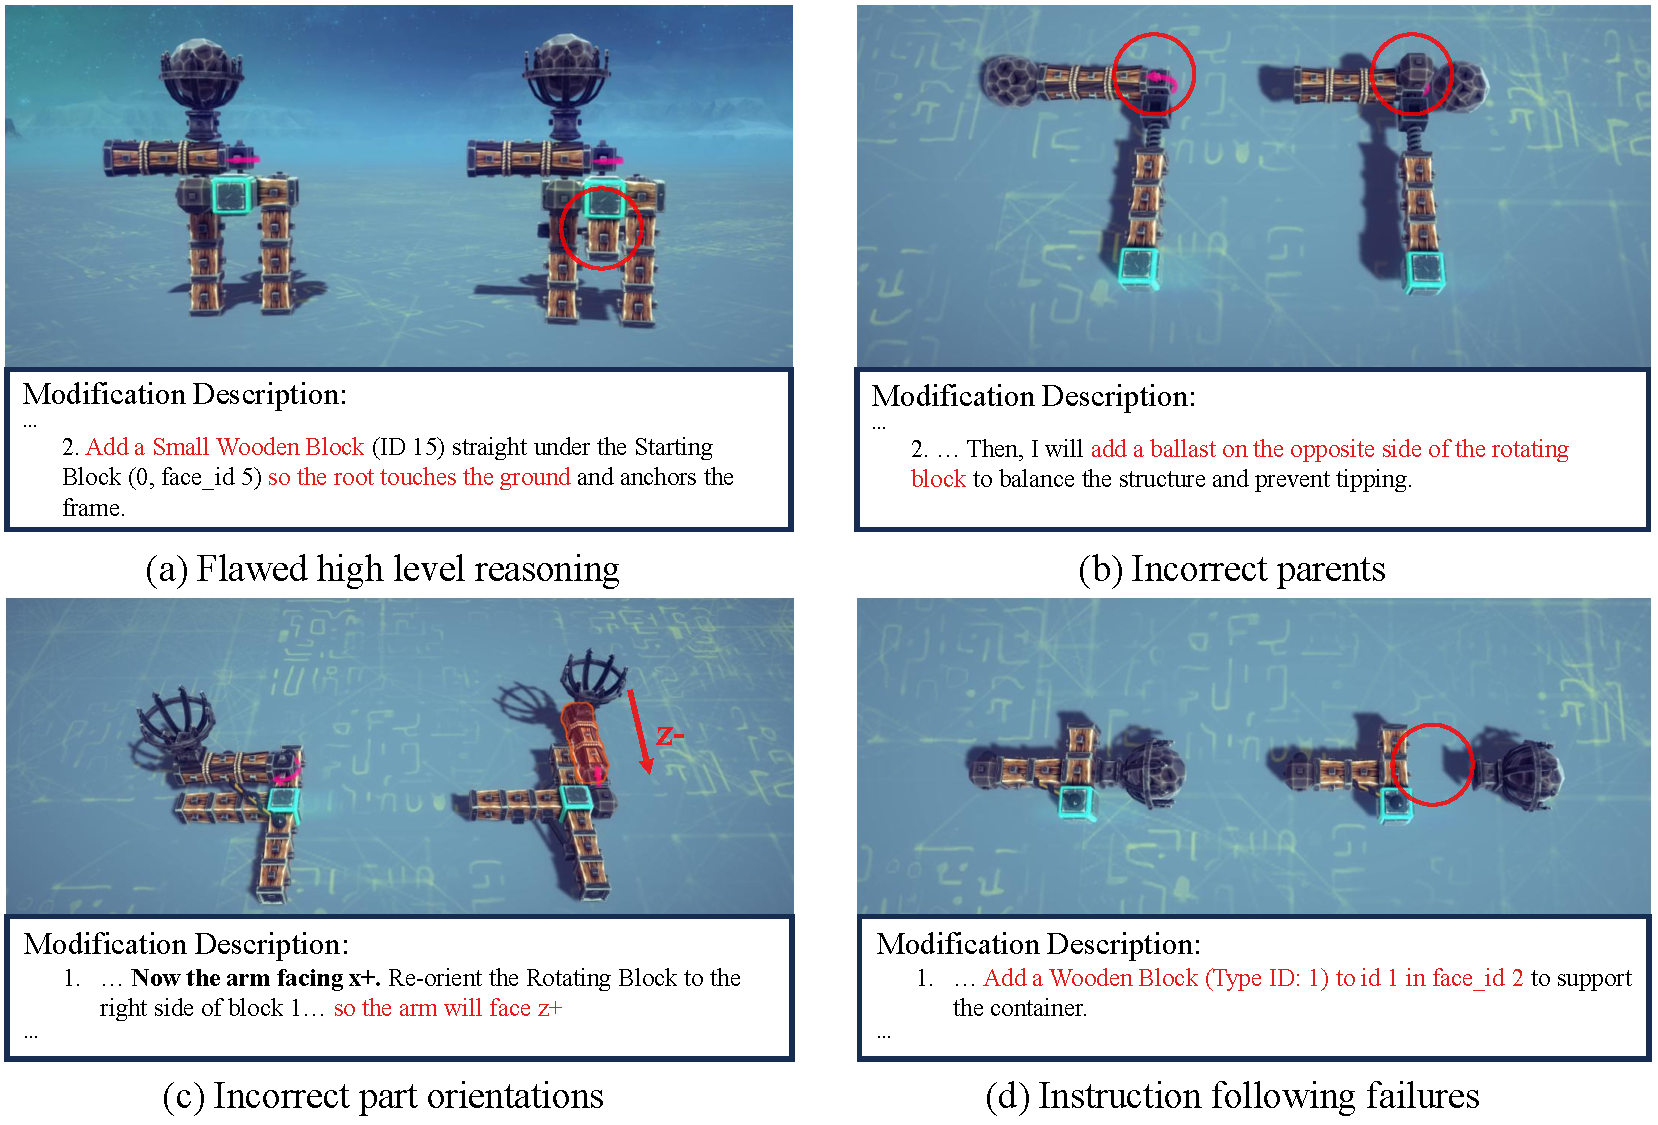
\includegraphics[width=\linewidth]{figures/failure_mode_v3_cropped.pdf}
  \caption{\footnotesize Examples to illustrate failure patterns. In each example, the original machine is shown on the left and the modified machine on the right. Failure patterns are sampled from Qwen3-Coder-480B-A35B-Instruct.}
  \label{fig:failure-mode}
\end{figure}


\subsection{Need for Precision}


In Fig.~\ref{fig:tiny-modify} we present a simple example to illustrate how the task of compositional machine design requires high precision in the spatial design of configurations of different parts. Even though the high-level design is feasible, the machine in the top row fails to throw the boulder out due to the incorrect position of the container.


\begin{figure}[h!]
  \centering
  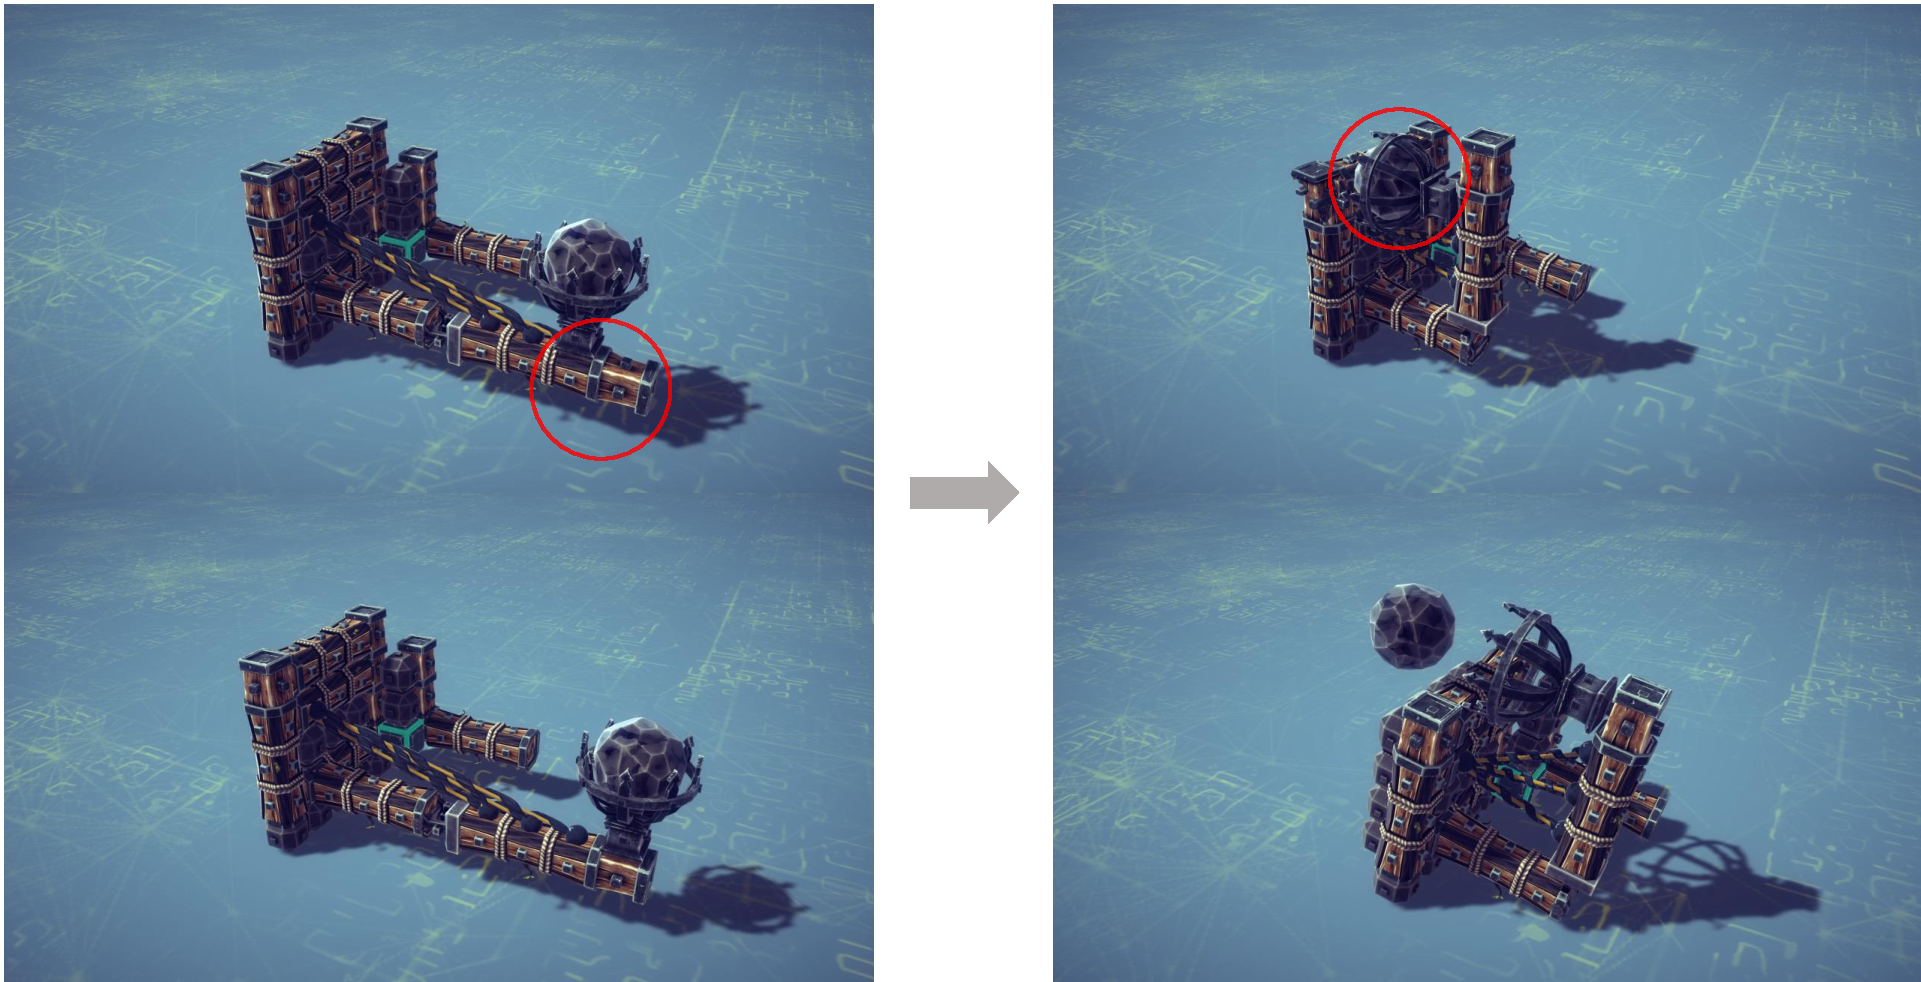
\includegraphics[width=\linewidth]{figures/tiny_modify_v3_cropped.pdf}
  \caption{\footnotesize Illustration of how machines built with feasible high-level designs may fail due to inaccurate part placement. Machine sampled from Gemini 2.5 Pro. Left: designed machines; Right: simulation results.}
  \label{fig:tiny-modify}
\end{figure}

\subsection{Appearance vs.~Performance}

As illustrated in Fig.~\ref{fig:throw-traj}, a machine's appearance does not necessarily reflect its actual performance. A design that seems well-aligned with human intuition can fail dramatically, while one that looks awkward or unintuitive may achieve superior results. For LLMs to design machines that are both effective and visually intuitive to humans, reward functions must account not only for task performance but also for stability and other factors that shape human perception of functionality.

\begin{figure}[h!]
  \centering
  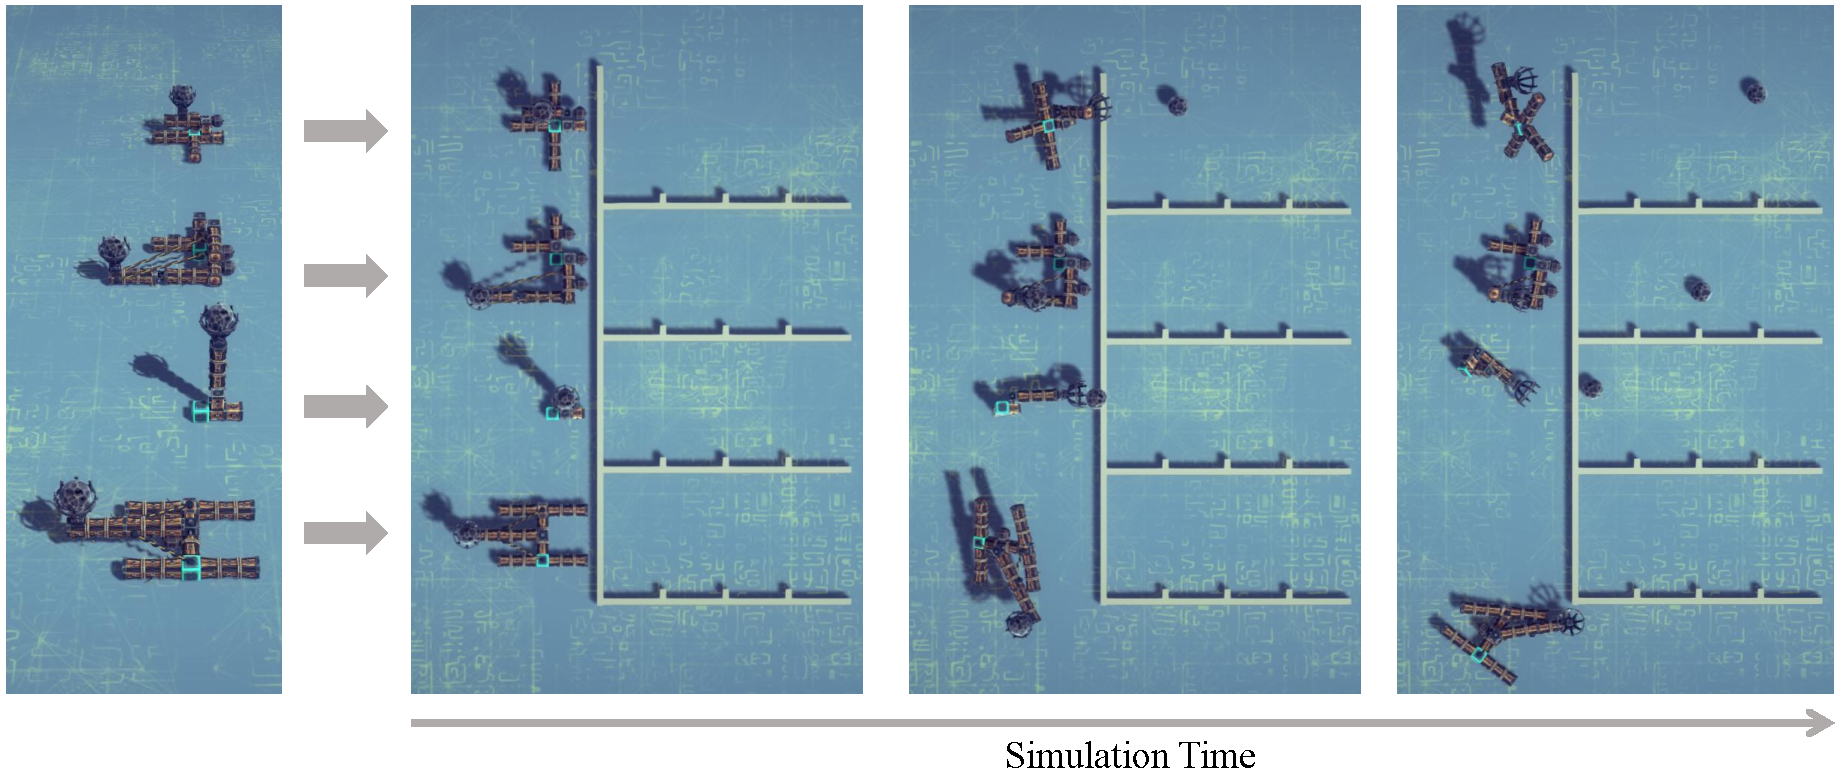
\includegraphics[width=\linewidth]{figures/throw_comp_v4_cropped.pdf}
  \caption{\footnotesize Boulder-throwing trajectories for various machine designs generated by Gemini 2.5 Pro. From left to right, each row first shows the machine design, followed by a time-lapsed bird’s-eye view of its throw.}
  \label{fig:throw-traj}
\end{figure}


\clearpage
\newpage
\section{Settings for RL Finetuning}



\subsection{Cold-Start Dataset Curation} \label{sec:cold_start_data} 


Noticing that Gemini 2.5 Pro produces the most satisfactory machines with reasonable CoT, we adopt the single-agent generation setting and collect Gemini-generated machines along with their CoT. We curated 100 design objectives: 75 captions of machines created by Besiege players from the Internet and 25 authored by us. These 25 prompts are constructed by 1) first writing down simple design objectives that are realizable by \envname and can emerge from some simple rewards, and 2) then introducing environment constraints and machine-specific requirements. Using this prompt dataset, we generate 250 machines per prompt, and after filtering out inappropriate ones (those that fail to parse, cannot be built in the environment, or do not have a specific physics-driven functionality, \eg, a statue), we obtain 9,984 machines with their corresponding CoT. A sample gallery is shown in Fig.~\ref{fig:synthesized_dataset}.


We present examples in the curated prompt set: 
\begin{lstlisting}
1. Build a machine that can provide an exciting spinning amusement ride experience.
2. Build a machine that can mimic the movements of a humanoid figure for entertainment or functional demonstrations.
3. Build a machine that can glide smoothly over snow or ice.
\end{lstlisting}

Below we present the text prompts with our simple authoring strategy, which can possibly be scaled with LLMs:
\begin{lstlisting}
-Additional Environment Constraints-
1. On an uneven, bumpy straight road, build a small car that must travel in a straight line to the finish.
2. On a straight road stands a stone wall; build a battering ram that must accelerate straight ahead, smash the wall, and finish with minimal damage to the machine.
-Modified Demands for Target Machines-
1. Build a tall tower that must keep a heavy block (id 36) at 15 m height for 5 s without collapse.
2. On a straight road stands a 10 m high wall; build a siege ladder that must advance, extend its top above the wall, and remain upright throughout.
\end{lstlisting}





\begin{figure}[h!]
  \centering
  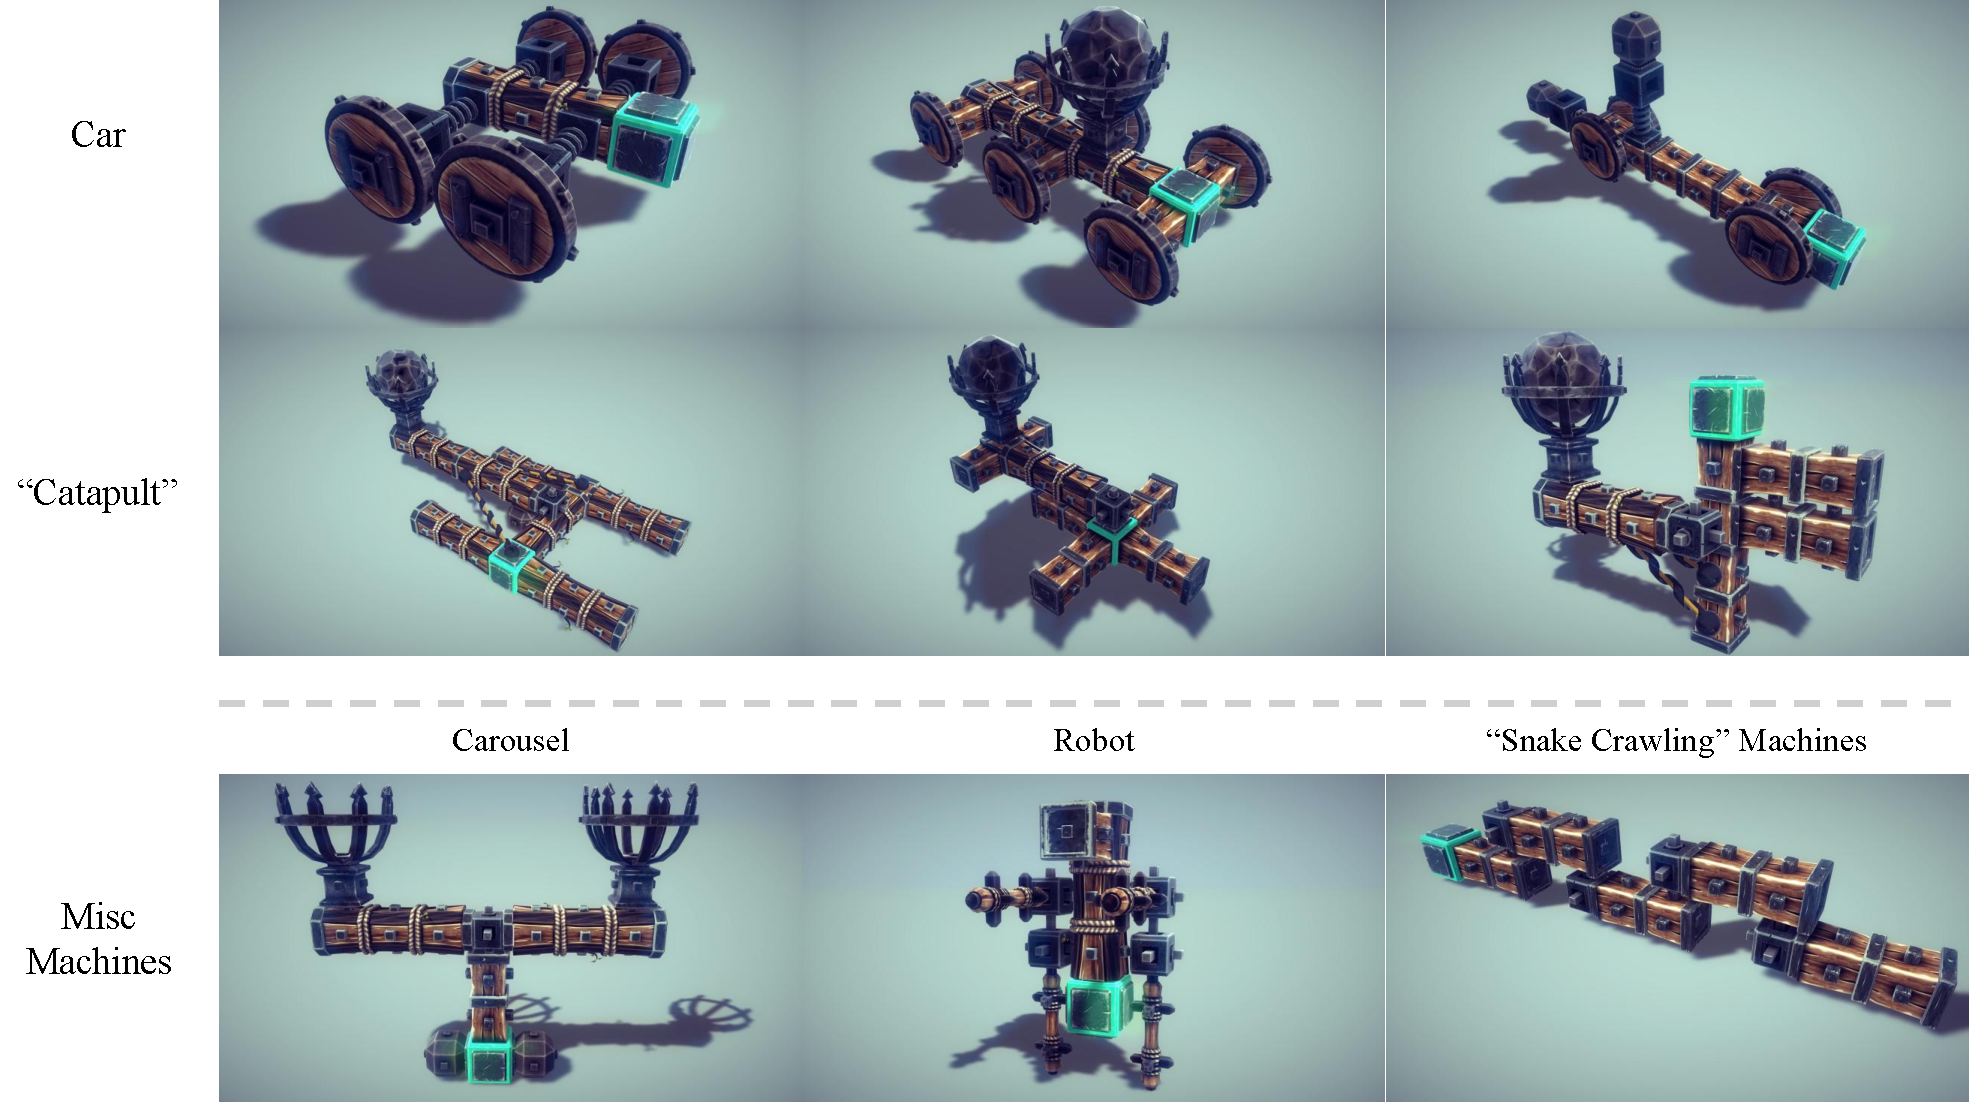
\includegraphics[width=\linewidth]{figures/synthesised_dataset_v3_cropped.pdf}
  \caption{\footnotesize Examples of Gemini-synthesized machines.}
  \label{fig:synthesized_dataset}
\end{figure}


























\subsection{Cold-Start Details} \label{sec:cold_start_details}

In our experiment, we use Qwen2.5-14B-Instruct as the base model and train it on the Gemini synthesized dataset. To save GPU memory, we employ the parameter-efficient quantized OFT (QOFT) technique~\citep{qiu2025oftv2, qiu2023controlling, liu2024boft, qiu2025reparameterized} for updating the model parameters, with OFT block size 64. We use 8-bit training with the 8-bit AdamW optimizer implmented with bitsandbytes~\citep{dettmers20228bit}, a learning rate of 1e-6 and a linear warmup schedule (3\% of the total training steps).





\subsection{RL Experiment Details}
\label{sec:rl_exp_details}
We use verl framework to implement our RL experiments. The LLM is finetuned from Qwen2.5-14B-Instruct (with LoRA of rank 64 on all linear layers) using the Gemini-synthesized dataset described above. We set learning rate to 5e-6 with gradient clipping threshold set to 0.5. The GRPO advantage estimator uses an advantage clipping ratio of 0.2. We add a KL penalty (weight 0.001) with respect to the pretrained LLM and do not introduce any entropy regularization. For rollouts, we use a temperature of $1.0$ and top-$p$ value of 0.95. Maximum input and output lengths are 3440 and 1168 tokens, respectively. We train each model for 400 update steps which take approximately 48 hours.










\clearpage
\newpage
\section{Additional Ablation Studies}

\textbf{Meta-Designer in hierarchical design.} In Table~\ref{tab:ablation_meta_designer}, we show that how a meta-designer for hierarchical design may benefit compositional machine design. Leveraging the knowledge on existing machines, meta-designers can identify the key macro-level mechanical components that are easier to design compared to the whole task, as shown in the results for Gemini 2.5 Pro, Kimi K2 and Llama 4 Scout. However, introducing an additional stage can introduce compounding error and, if the LLM agent is not capable of integrating different macro-level mechanical components, they may lead to lower scores, which we hypothesize is the reason for the failure of hierarchical design in models like Qwen3. Moreover, we examine if the meta-designer should provide step-by-step building instruction for the designer (Fig.~\ref{fig:detailed-meta-designer}), or simply provide high-level mechanical component descriptions. We find that a meta-designer that provides more detailed information is beneficial mostly when the base model is powerful enough (\eg, Gemini 2.5 Pro).

\textbf{Effect of feedback-free self-critic.} In Table~\ref{tab:ablation_inspector}, we show that the inspector agent which does self-critic before running any environment simulation tend to improve performance for models like Gemini 2.5 Pro (the most powerful model for the task of compositional machine design in \envname) but can fail drastically for models like o3.

\textbf{Effect of active feedback queries.} In Table~\ref{tab:rl_env_feedback}, we show that the active queries on the environment feedbacks help most of the models achieve better performance, compared to the setting with no environment feedback and that with only environment simulation final scores.

\textbf{Additional RL results.} In Fig.~\ref{fig:RL-catapult-max-score} and \ref{fig:RL-catapult-valid-rate} and , we show the maximum scores achieved in the environments with different RL methods plus the validity rate of machines. We visualize the maximum score since, in the case when one is allowed to use inference-time scaling techniques, the best performing machines are the ones people care most about. We show that our settings with Pass@64 training achieves the best maximum score with two different random seeds. In additiona, in Fig.~\ref{fig:RL-catapult-best@n}, we visualize the corresponding Best@N metrics.

For completeness, we also visualize the results with our default setting on the task \textit{car} in Fig.~\ref{fig:RL-car-max-score}, \ref{fig:RL-car-valid-rate} and \ref{fig:RL-car-best@n}.





\begin{table}[h!]
  \centering
  \setlength{\tabcolsep}{3pt}
  \renewcommand{\arraystretch}{1.1}
  \newcommand{\cgr}[1]{\textcolor[rgb]{.329, .51, .208}{\textbf{#1}}}
  \newcommand{\cre}[1]{\textcolor[rgb]{1, 0, 0}{\textbf{#1}}}
  \renewcommand{\pm}{\mathbin{\text{±}}}

  \begin{tabularx}{\textwidth}{lCCC>{\centering\arraybackslash}p{1.5cm}>{\centering\arraybackslash}p{1.5cm}}
    \toprule
    \multirow{2}{*}{Models}
    & \multicolumn{3}{c}{Machine Validity (pass/total)}
    & \multicolumn{2}{c}{Designer Score} \\
    \cmidrule(lr){2-4}\cmidrule(lr){5-6}
    & File Valid & 3D Valid & Final Valid & Mean & Max \\
    \midrule
    \multicolumn{6}{l}{\textit{Baseline (Meta-Designer \& Designer)}} \\
    \midrule
    Gemini 2.5 Pro    & 8/8 & 5/8 & 5/8 & 8.49 & 9.14 \\
    o3            & 3/8 & 3/3 & 3/8 & 0      & 0 \\
    Qwen3-Coder-480B-A35B    & 8/8 & 6/8 & 6/8 & 0.75 & 4.5 \\
    Doubao Seed 1.6    & 7/8 & 3/7 & 3/8 & 4.34 & 4.37 \\
    Claude Opus 4      & 8/8 & 4/8 & 4/8 & 4.17 & 4.36 \\
    DeepSeek-V3   & 7/8 & 7/7 & 7/8 & 0    & 0 \\
    Kimi K2       & 6/8 & 6/6 & 6/8 & 7.18 & 12.02 \\
    Llama 4 Scout 17B 16E        & 8/8 & 8/8 & 8/8 & 3.59      & 11.83 \\
    \midrule
    \multicolumn{6}{l}{\textit{Single Agent}} \\
    \midrule
    Gemini 2.5 Pro    & 6/8 & 3/6 & 3/8 & 6.13 & 9.00 \\
    o3            & 8/8 & 8/8 & 8/8 & 2.87 & 5.22 \\
    Qwen3-Coder-480B-A35B    & 8/8 & 4/8 & 4/8 & 3.5 & 9.24 \\
    Doubao Seed 1.6    & 7/8 & 6/7 & 6/8 & 4.24 & 8.2 \\
    Claude Opus 4      & 8/8 & 2/6 & 2/8 & 4.76 & 4.91 \\
    DeepSeek-V3   & 7/8 & 6/7 & 6/8 & 4.67 & 4.86 \\
    Kimi K2       & 8/8 & 3/8 & 3/8 & 6.85 & 9.05 \\
    Llama 4 Scout 17B 16E        & 8/8 & 7/8 & 7/8 & 3.63 & 5.64 \\
    \midrule
    \multicolumn{6}{l}{\textit{w/ detailed Meta-Designer \& Designer }} \\
    \midrule
    Gemini 2.5 Pro    & 8/8 & 7/8 & 7/8 & 9.19 &11.94 \\
    o3            & 7/8 & 6/7 & 6/8 & 0.92& 1.18 \\
    Qwen3-Coder-480B-A35B    & 8/8 & 2/8 & 2/8 & 4.87 & 4.87 \\
    Doubao Seed 1.6    & 0/8 & -   & -   & - & - \\
    Claude Opus 4      & 7/8 & 5/7 & 5/8 & 4.13 & 4.79 \\
    DeepSeek-V3   & 8/8 & 8/8 & 8/8 & 6.12 & 9.0 \\
    Kimi K2       & 8/8 & 0/8 & -   & - & - \\
    Llama 4 Scout 17B 16E        & 8/8 & 7/8 & 7/8 & 4.01 & 6.93 \\
    \bottomrule
  \end{tabularx}
  \caption{\footnotesize Ablation study on the meta-designer. Machine validity is evaluated in two aspects: file validity, 3D validity. Note that 3D validity requires the machine to first pass file validity. Final validity refers to a fully valid machine (satisfying both file and 3D validity). The mean simulation score is calculated based solely on the final valid outputs. \textit{Detailed Meta-Designer} provides more concisely, step-by-step construction guidance to the \textit{Designer}.  Compared to \textit{Baseline}, \textit{Single Agent} is slightly harder to construct valid machines, but the simulation scores are better. \textit{Detailed Meta-Designer} improves both metrics, but requires LLMs to have a strong 3D understanding and a large context window. The comparison between \textit{Meta-Designer} and \textit{Detailed Meta-Designer} is illustrated in Fig.~\ref{fig:detailed-meta-designer}.}
  \label{tab:ablation_meta_designer}
\end{table}

\begin{figure}[h!]
  \centering
  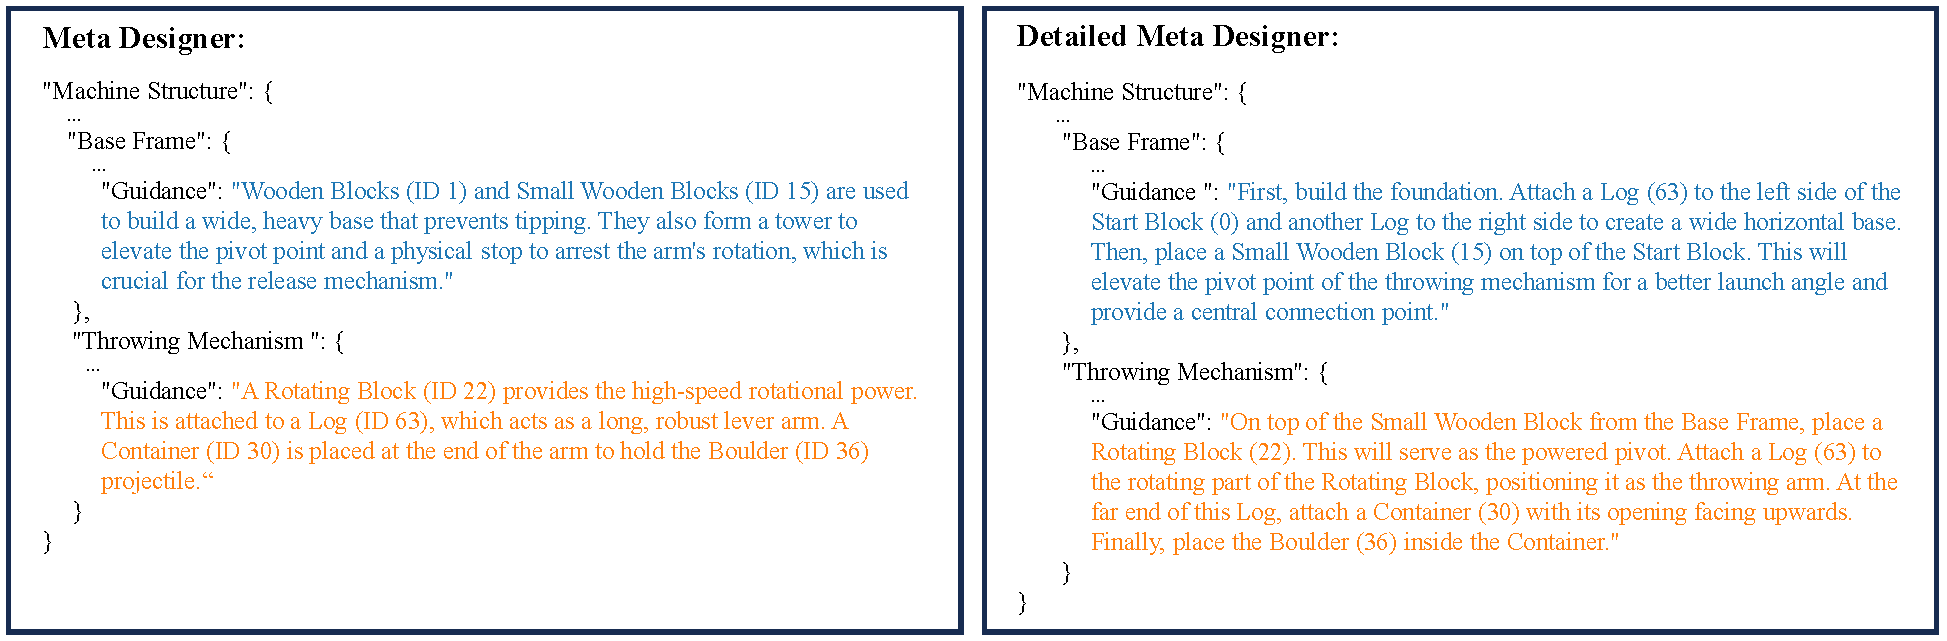
\includegraphics[width=\linewidth]{figures/designer_detailed_designer_cropped.pdf}
  \caption{\footnotesize Construction guidance comparison of \textit{Meta Designer} and \textit{Detailed Meta Designer}, sampled with Gemini 2.5 Pro.}
  \label{fig:detailed-meta-designer}
\end{figure}

\begin{table}[h!]
  \centering
  \setlength{\tabcolsep}{3pt}
  \renewcommand{\arraystretch}{1.1}
  \newcommand{\cgr}[1]{\textcolor[rgb]{.329, .51, .208}{\textbf{#1}}}
  \newcommand{\cre}[1]{\textcolor[rgb]{1, 0, 0}{\textbf{#1}}}

  \begin{tabularx}{\textwidth}{l*{6}{>{\centering\arraybackslash}X}}
    \toprule
    \multicolumn{1}{c}{\multirow{2.4}{*}{Models}}
    & \multicolumn{6}{c}{Blind Refinement Simulation Scores} \\
    \cmidrule(lr){2-7}
    & \multicolumn{3}{c}{Baseline}
    & \multicolumn{3}{c}{w/o Inspector} \\
    \cmidrule(lr){2-4}\cmidrule(lr){5-7}
    & Valid & Mean & Max & Valid & Mean & Max \\
    \midrule
    Gemini 2.5 Pro
       & 5 & \bf 8.18 & \bf 11.07
       & 5 & 5.67 & 9.37 \\
    o3
       & 3 &0 & 0
       & 3 &\bf 3.08  & \bf 9.24 \\
    Qwen3-Coder-480B-A35B
       & 6 & \bf 1.61 & \bf 5.0
       & 6 & 0.75 & 4.51\\
    Doubao Seed 1.6
       & 3 & 0.31 & \bf 0.49
       & 3 & \bf 0.47 &1.41  \\
    Claude Opus 4
       & 2 &\bf 5.38  &5.8 
       & 4 &5.20  & \bf 8.25  \\
    DeepSeek-V3
       & 7 & \bf 0.98 & \bf 3.18
       & 7 &0.38  &2.16  \\
    Kimi K2
       & 2 & \bf 5.29 &7.36 
       & 6 & 2.31 & \bf 8.91 \\
    Llama 4 Scout 17B 16E
       & 0 & - & -
       & 0 & - & - \\
    \bottomrule
  \end{tabularx}
    \caption{\footnotesize Ablation study on inspector agentic design. The mean simulation score is calculated based solely on the valid machines after blind refinement. Removing the inspector from the agentic flow lowers the blind refiner’s mean performance on LLMs with weaker 3D understanding, while barely affecting other models.}
  \label{tab:ablation_inspector}
\end{table}


\begin{table}[h!]
  \centering
  \setlength{\tabcolsep}{3pt}
  \renewcommand{\arraystretch}{1.1}
  \newcommand{\cgr}[1]{\textcolor[rgb]{.329, .51, .208}{\textbf{#1}}}
  \newcommand{\cre}[1]{\textcolor[rgb]{1, 0, 0}{\textbf{#1}}}

  \begin{tabularx}{\textwidth}{l*{9}{>{\centering\arraybackslash}X}}
    \toprule
    \multicolumn{1}{c}{\multirow{2.4}{*}{Models}}
    & \multicolumn{9}{c}{Refiner Simulation Scores} \\
    \cmidrule(lr){2-10}
    & \multicolumn{3}{c}{Baseline}
    & \multicolumn{3}{c}{w/o Env Querier}
    & \multicolumn{3}{c}{Score Only}\\
    \cmidrule(lr){2-4}\cmidrule(lr){5-7}\cmidrule(lr){8-10}
    & std & Mean & Max & std & Mean & Max& std & Mean & Max \\
    \midrule
    Gemini 2.5 Pro
       & 2.47 &\bf 15.73  &18.19 
       & 4.18 &14.89  &\bf 19.77
       & 2.05 &9.68  &13.18\\
    o3
       & 5.36 &5.34  & \bf 11.11
       & 4.24 &4.06  &8.55
       & 2.76 &\bf 7.05  &10.24\\
    Qwen3-Coder-480B-A35B
       & 0.95 & \bf 5.21 & \bf 6.52
       & 2.32 &4.05 &6.89 
       & 2.53 &2.81 &5.56\\
    Claude Opus 4
       & 0.31 &\bf 9.10 & \bf 9.32
       & 0.82 &8.50  &9.08
       & 0.42 &5.75  &6.05\\
    Doubao Seed 1.6
       & 0.23 &4.62  & 4.76
       & 0.08 &\bf 4.89 &4.94
       & 0.29 &4.79 &\bf 5.05\\
    DeepSeek-V3
       & 0.09 &\bf 4.82  & 4.93
       & 1.96 &4.37  &\bf 6.00
       & 1.91 &2.76  &5.15\\
    \bottomrule
  \end{tabularx}
  \caption{\footnotesize Ablation study on the environment querier agent. For the refiner, the baseline includes simulation scores, basic environment feedback, and querier-required feedback. The "w/o env querier" setting provides only simulation scores and basic environment feedback. In the "pure score only" setting, only simulation scores are provided. Removing the environment querier causes a slight drop in average machine performance. With reward signals only, the performance markedly degrades across most LLMs.}
  \label{tab:rl_env_feedback}
\end{table}




    

\begin{figure}[h!]
  \centering
  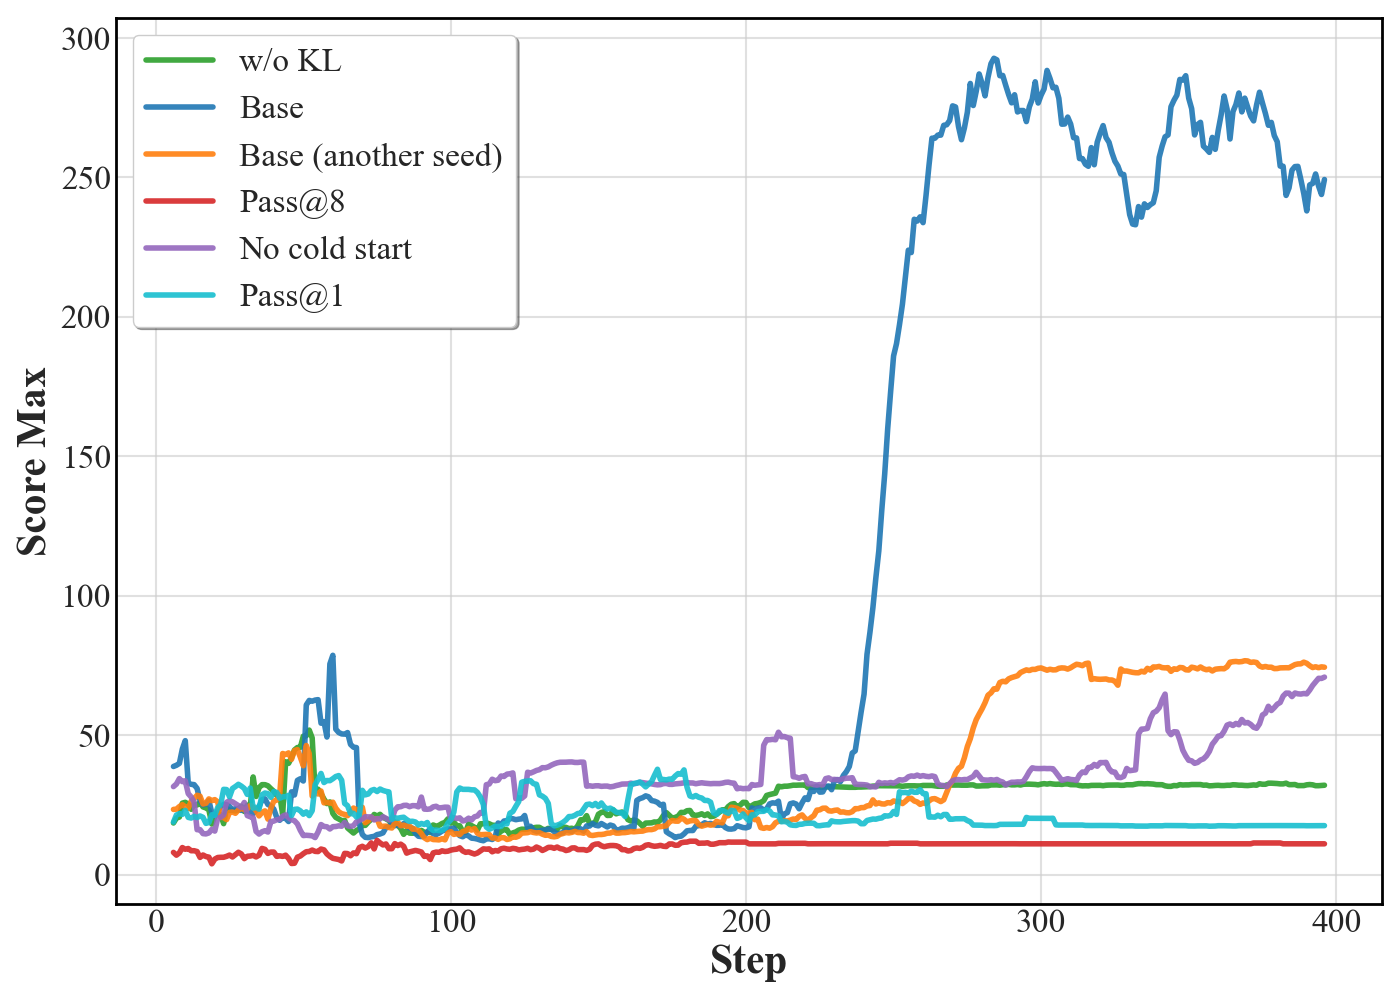
\includegraphics[width=0.5\linewidth]{figures/RL_Metrics/Catapult/score_max.png}
  \caption{\footnotesize \textit{Catapult} task machine scores across RL steps. KL regularization helps the model discover better structure designs. Pass@64 is greatly more efficient at uncovering powerful machine designs. Pass@8 (roll-out 8) outperforms Pass@1 (roll-out 64) in efficiency and matches its performance with fewer roll-outs. No cold start models lack the advanced knowledge needed to find better machines.} \label{fig:RL-catapult-max-score}
\end{figure}

\begin{figure}[h!]
    \centering
    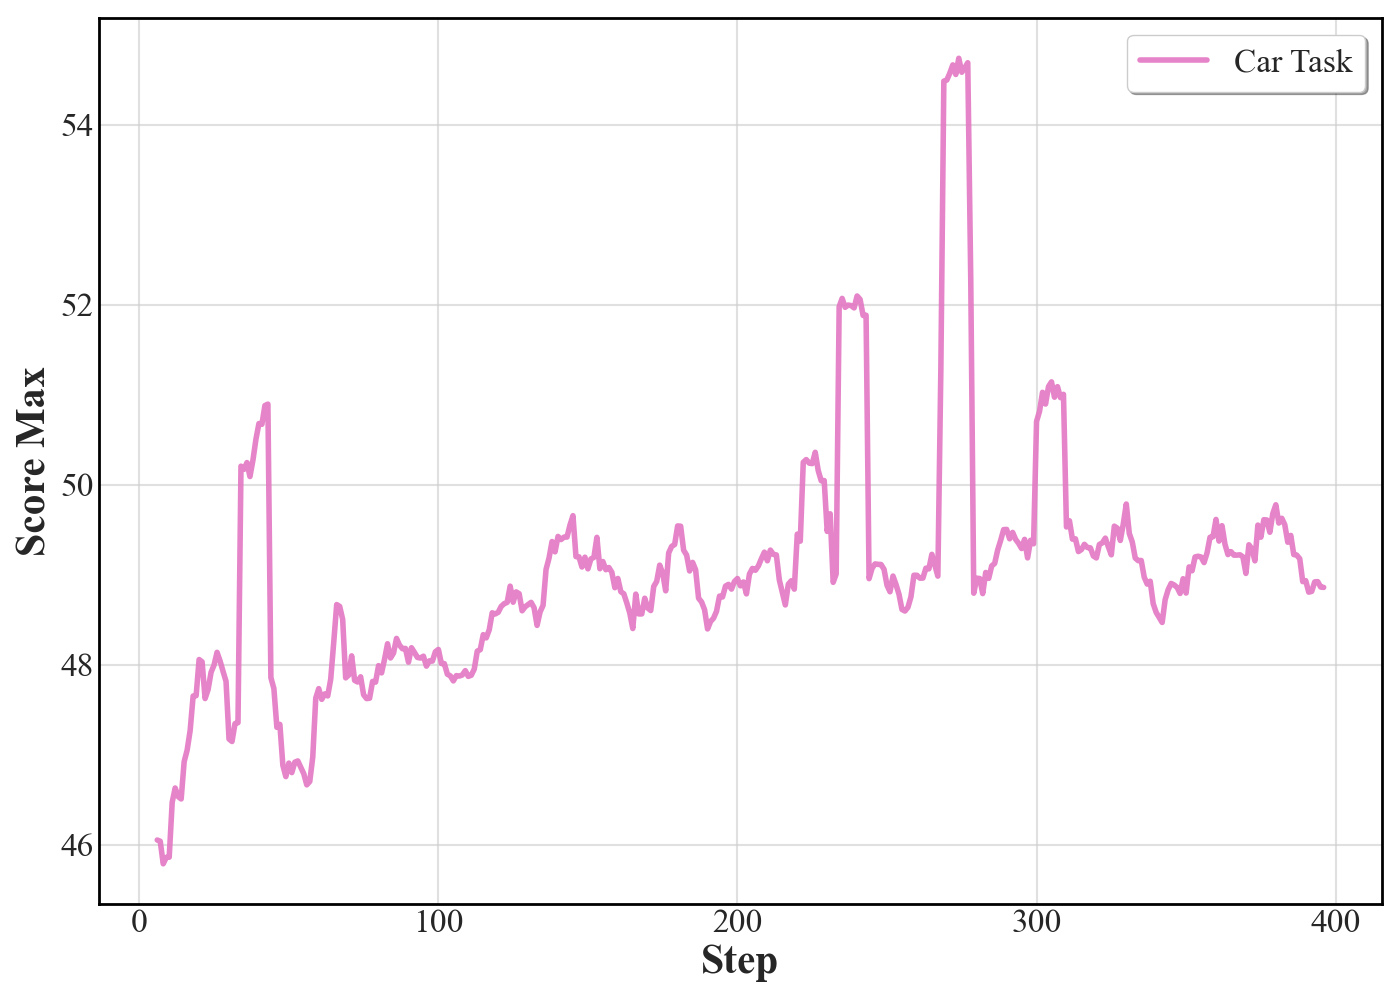
\includegraphics[width=.5\linewidth]{figures/RL_Metrics/Car/score_max.png}
    \caption{\footnotesize \textit{Car} machine scores across RL steps. The RL finetuning hyperparameter setting is the same as the base hyperparameter setting of \textit{Catapult}. Machine performance slightly rises as training steps increase.}
    \label{fig:RL-car-max-score}
\end{figure}


\begin{figure}[h!]
  \centering
  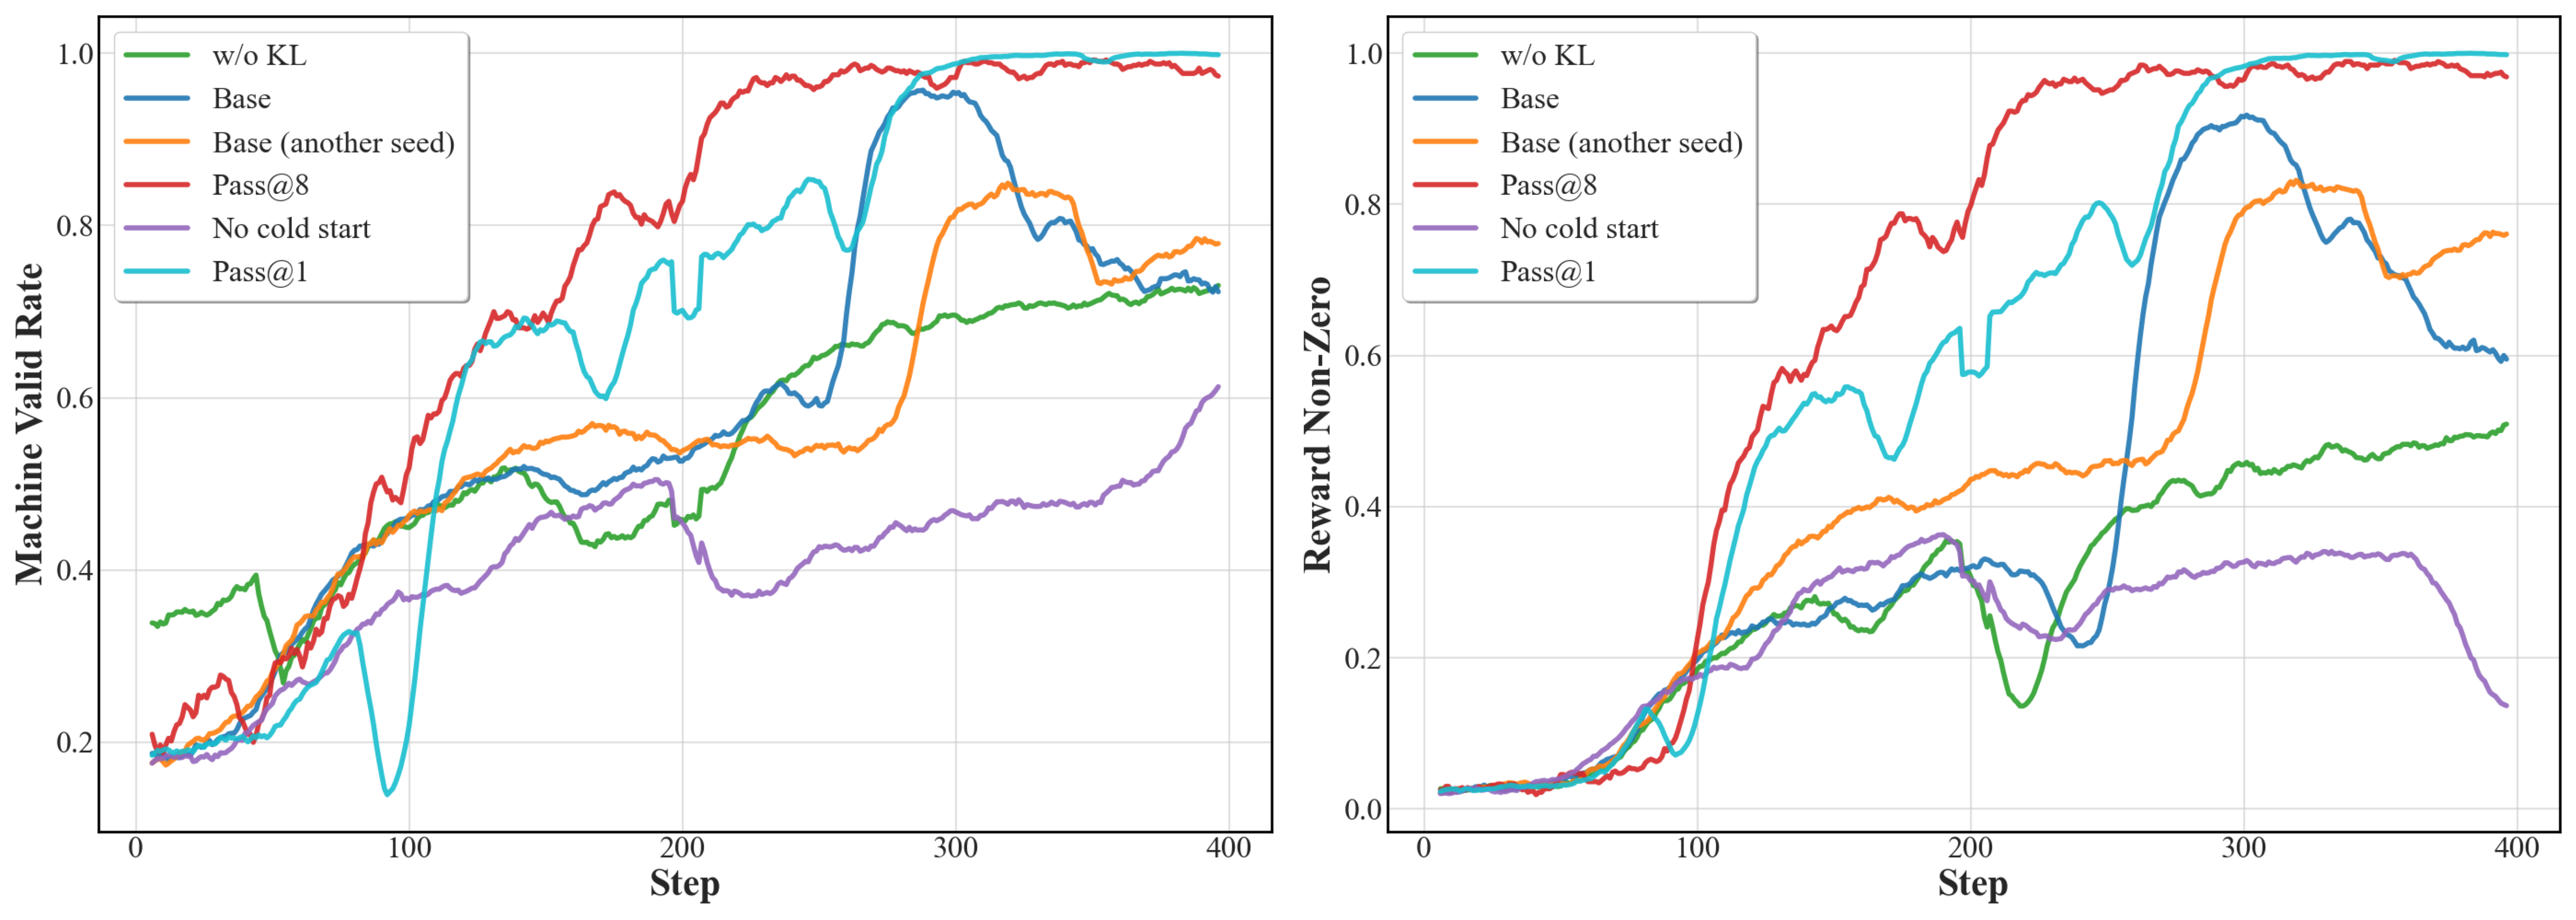
\includegraphics[width=\linewidth]{figures/RL_Metrics/Catapult/MachineValid_Reward.png}
  \caption{\footnotesize \textit{Catapult task} machine validity rate and reward non-zero rate across RL steps. The machine validity rate refers to the proportion of machines that can successfully run simulations. The reward non-zero rate represents the ratio of machines that can simulate with a non-zero reward. LLM constructs more legal machines as training steps increase, and rewards non-zero machines. Pass@8 and Pass@1 converge early. ``No KL'' fills roll-outs with failure cases, slowing performance gains. ``No cold start'' lacks design knowledge, encounters more failures than no KL, and improves validity rate most slowly. The base setting balances convergence and performance improvement.}
  \label{fig:RL-catapult-valid-rate}
\end{figure}


\begin{figure}[h!]
  \centering
  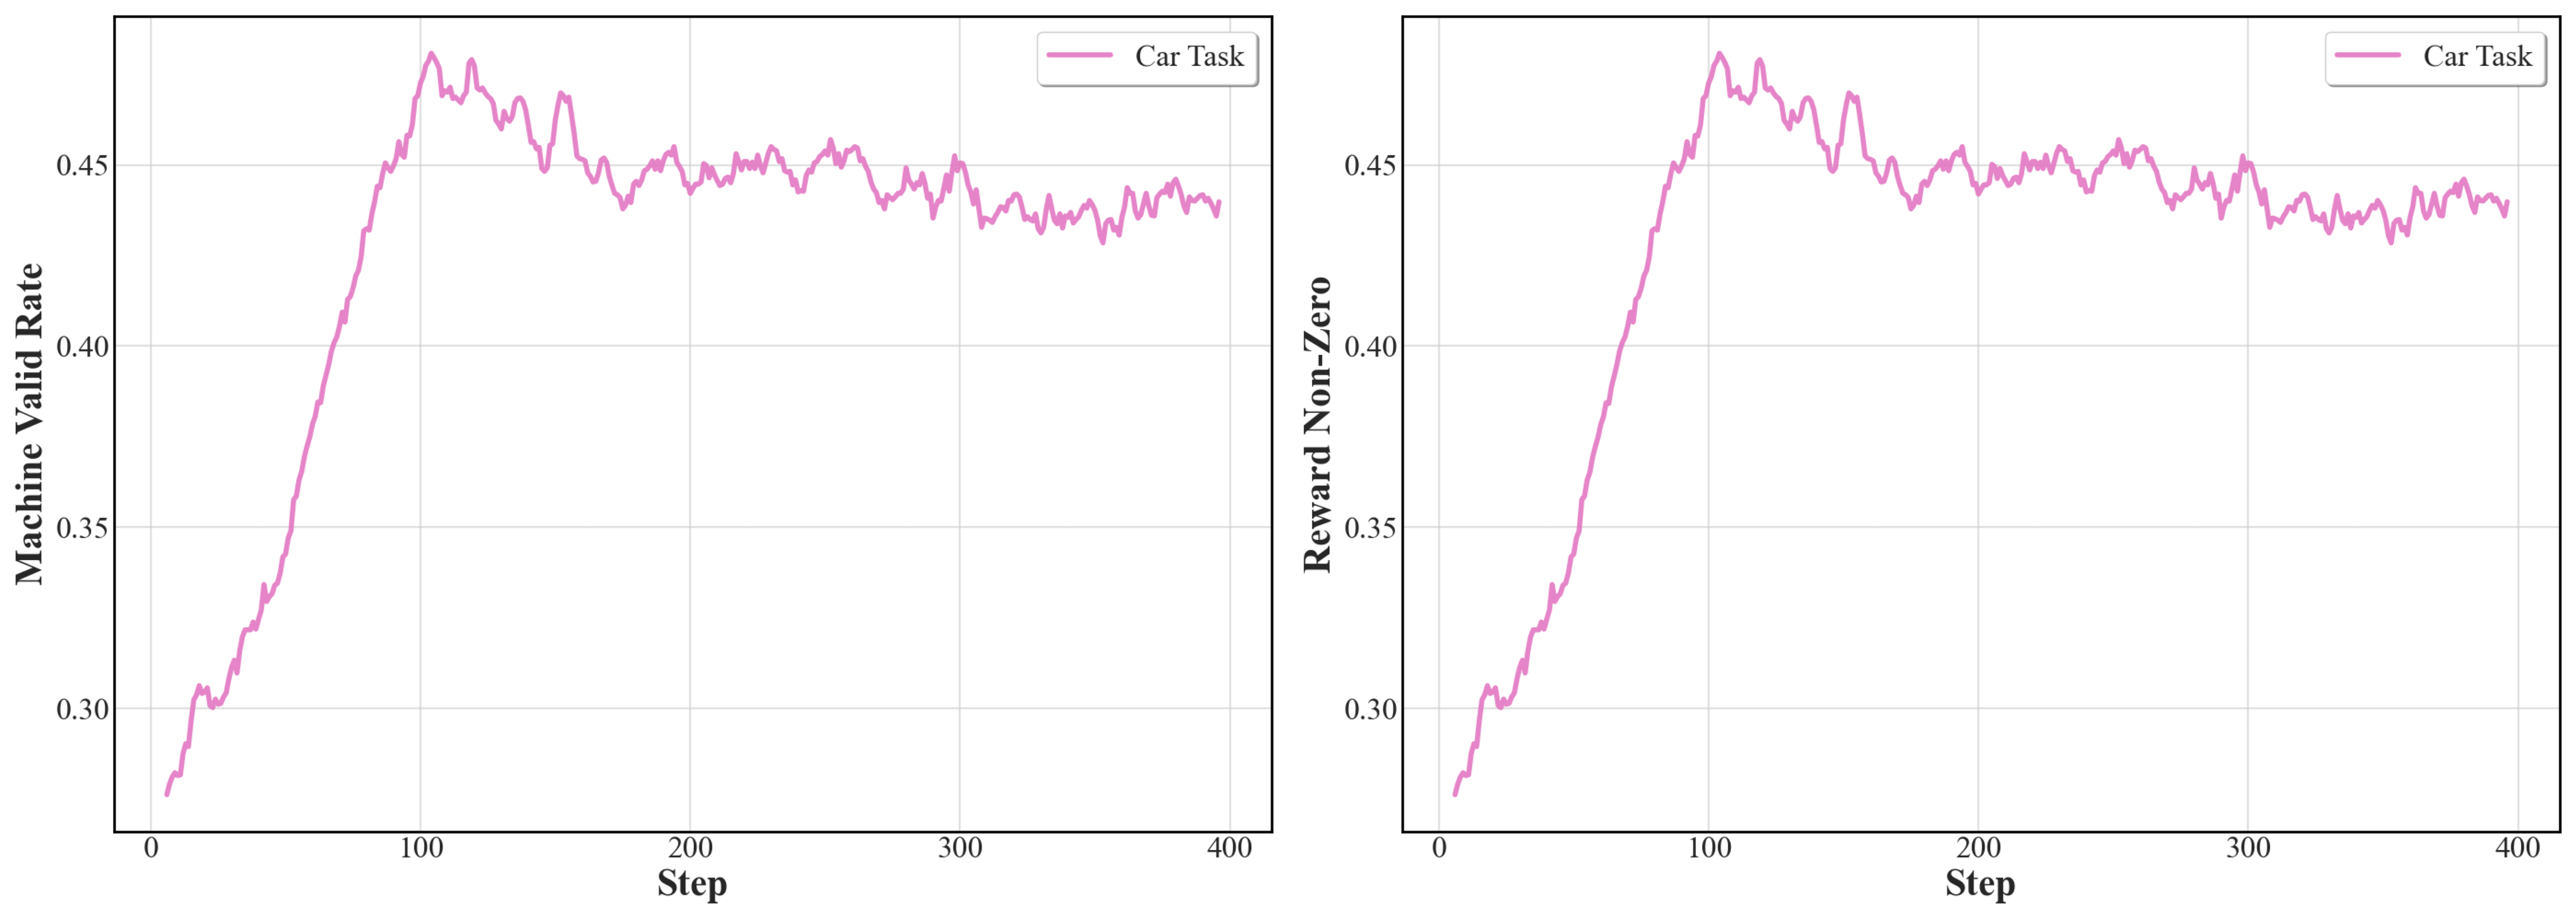
\includegraphics[width=\linewidth]{figures/RL_Metrics/Car/MachineValid_Reward.png}
  \caption{\footnotesize \textit{Car task} machine validity rate and reward non-zero rate across RL steps. The machine validity converges early and remains stable during further training.} \label{fig:RL-car-valid-rate}
\end{figure}


\begin{figure}[h!]
  \centering
  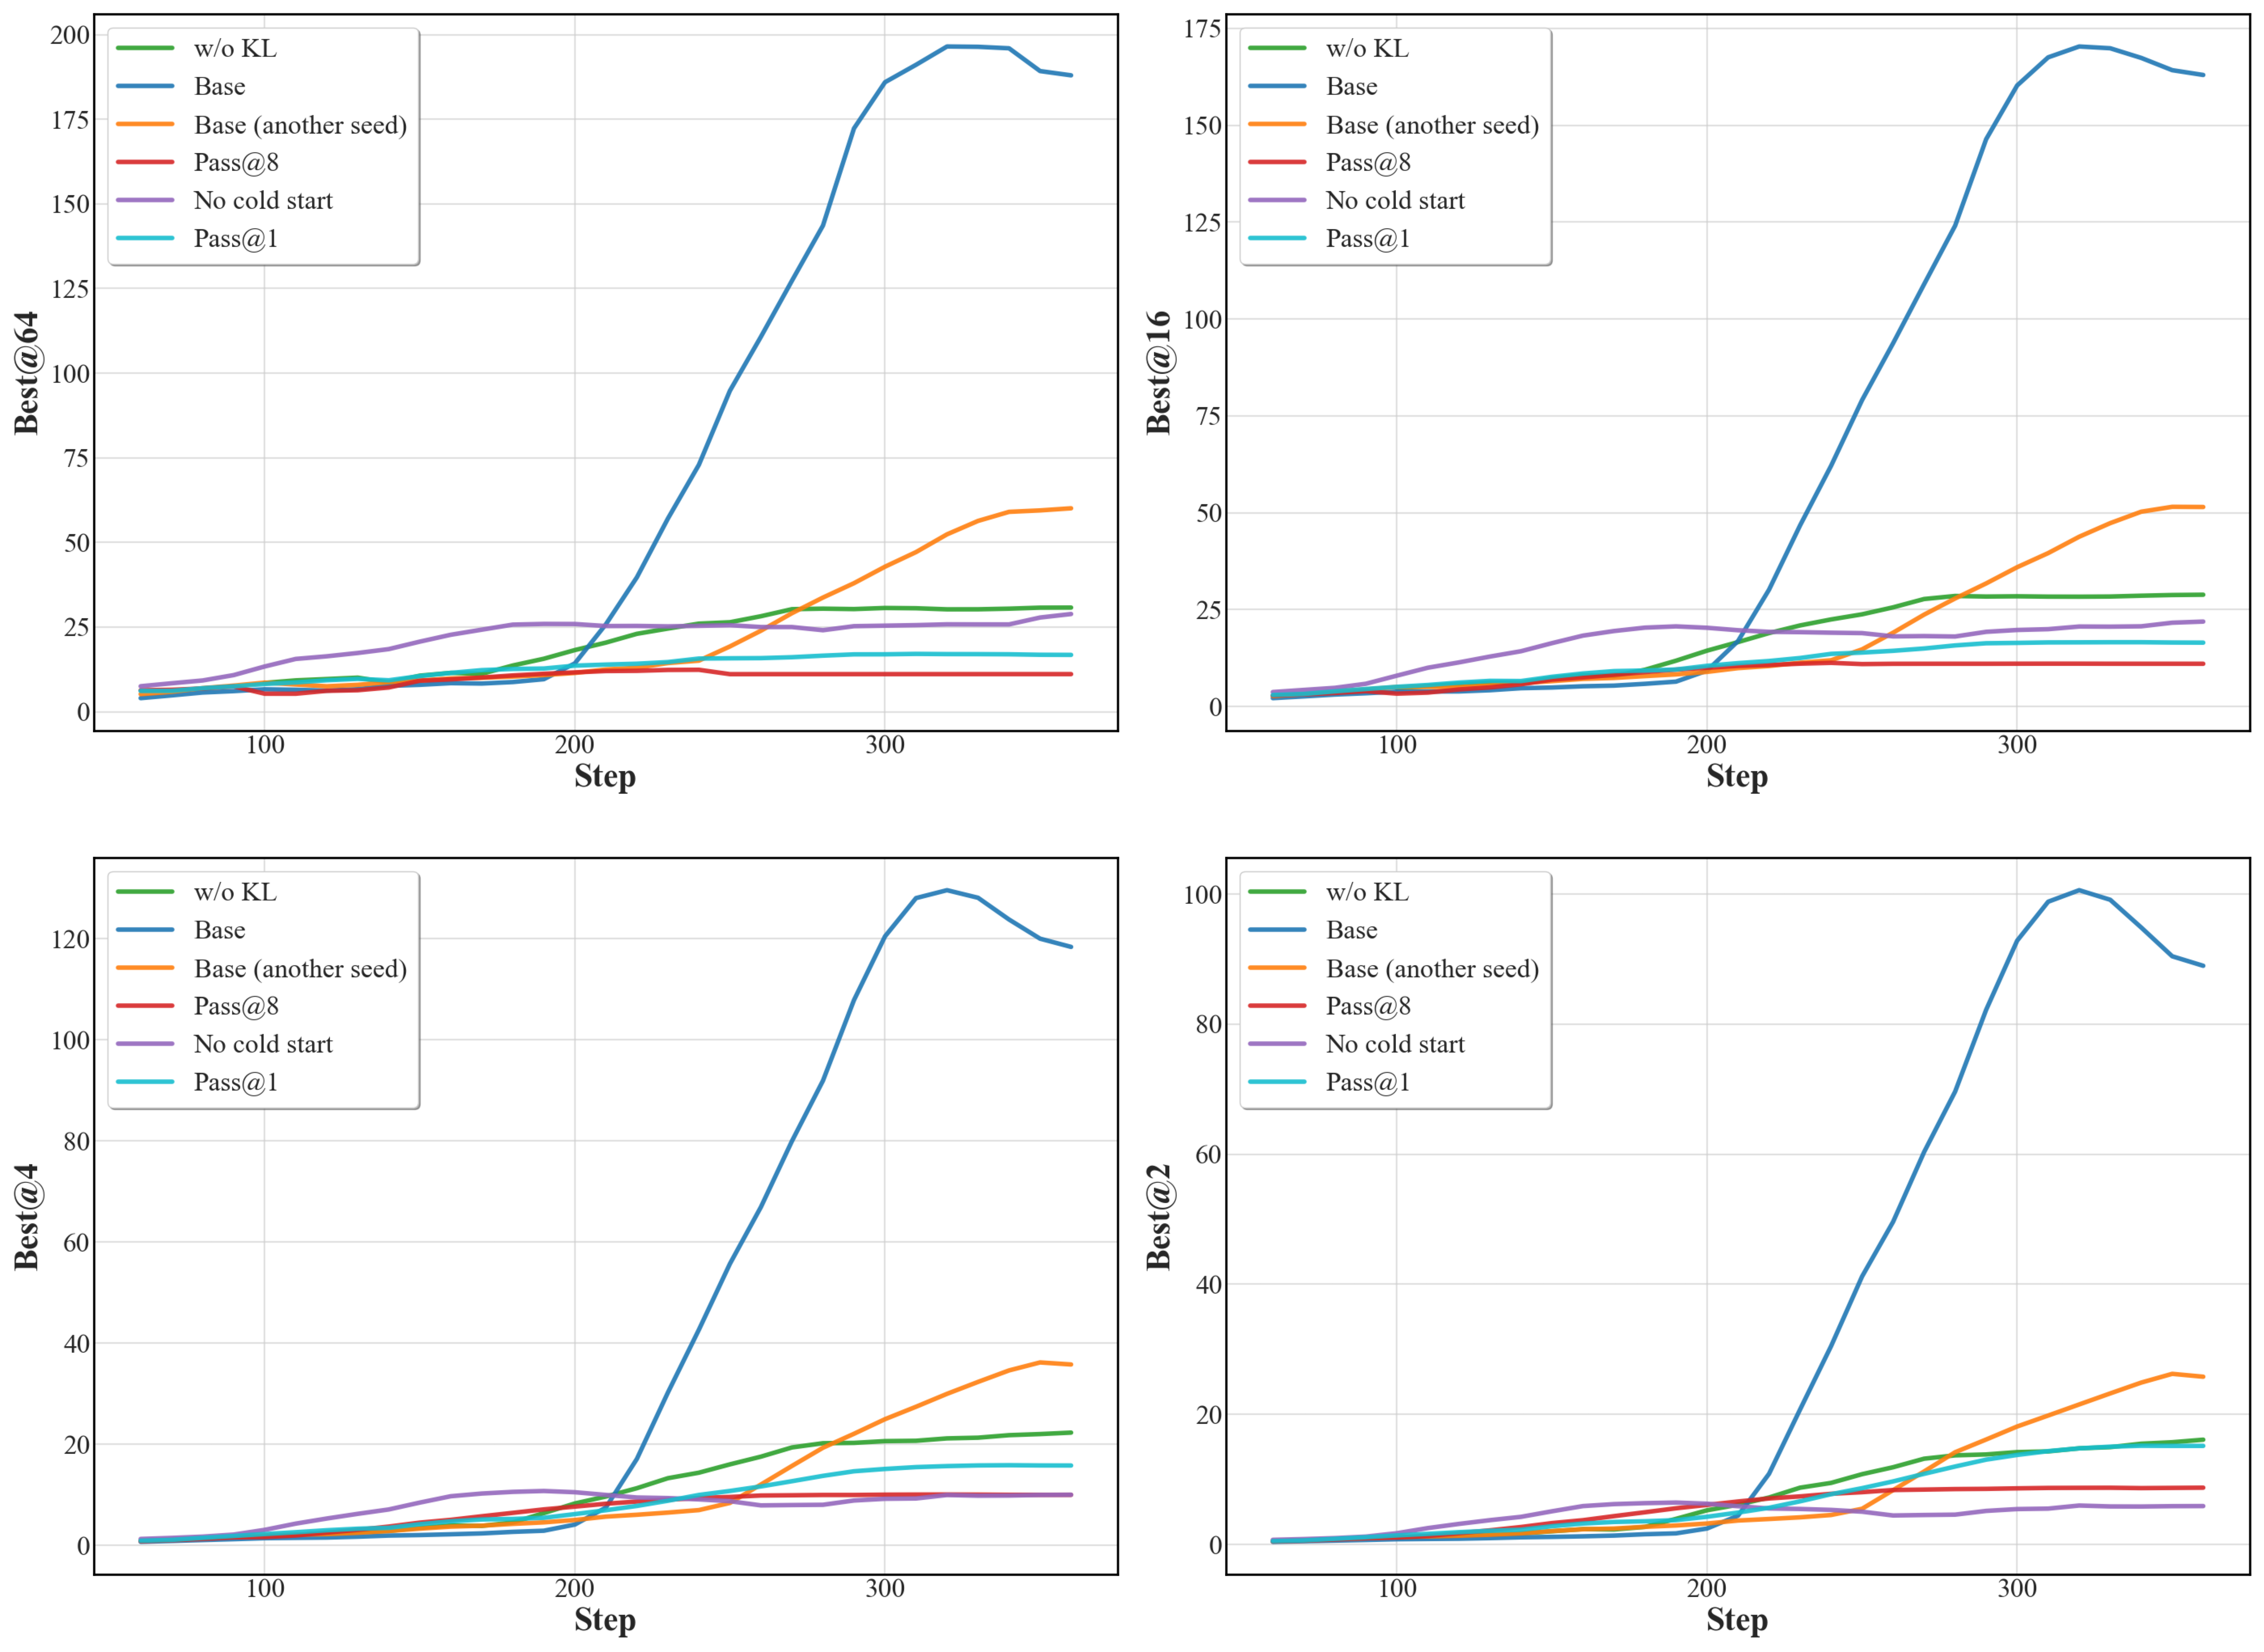
\includegraphics[width=\linewidth]{figures/RL_Metrics/Catapult/Val_Best.png}
  \caption{\footnotesize \textit{Catapult task}. Average Best@N metric. At each test step, the LLM generates 64 samples, selects the top $N$ samples, and records the maximum score. This process is repeated 1,000 times, and the mean value is calculated. Base settings (both seeds) dominates Best@N performance; excluding base settings, ``no KL'' dominates the rest. Pass@1 and Pass@8 spawn only a handful of high-performance machines. No cold start produces machines of more average quality.}
  \label{fig:RL-catapult-best@n}
\end{figure}

\begin{figure}[h!]
  \centering
  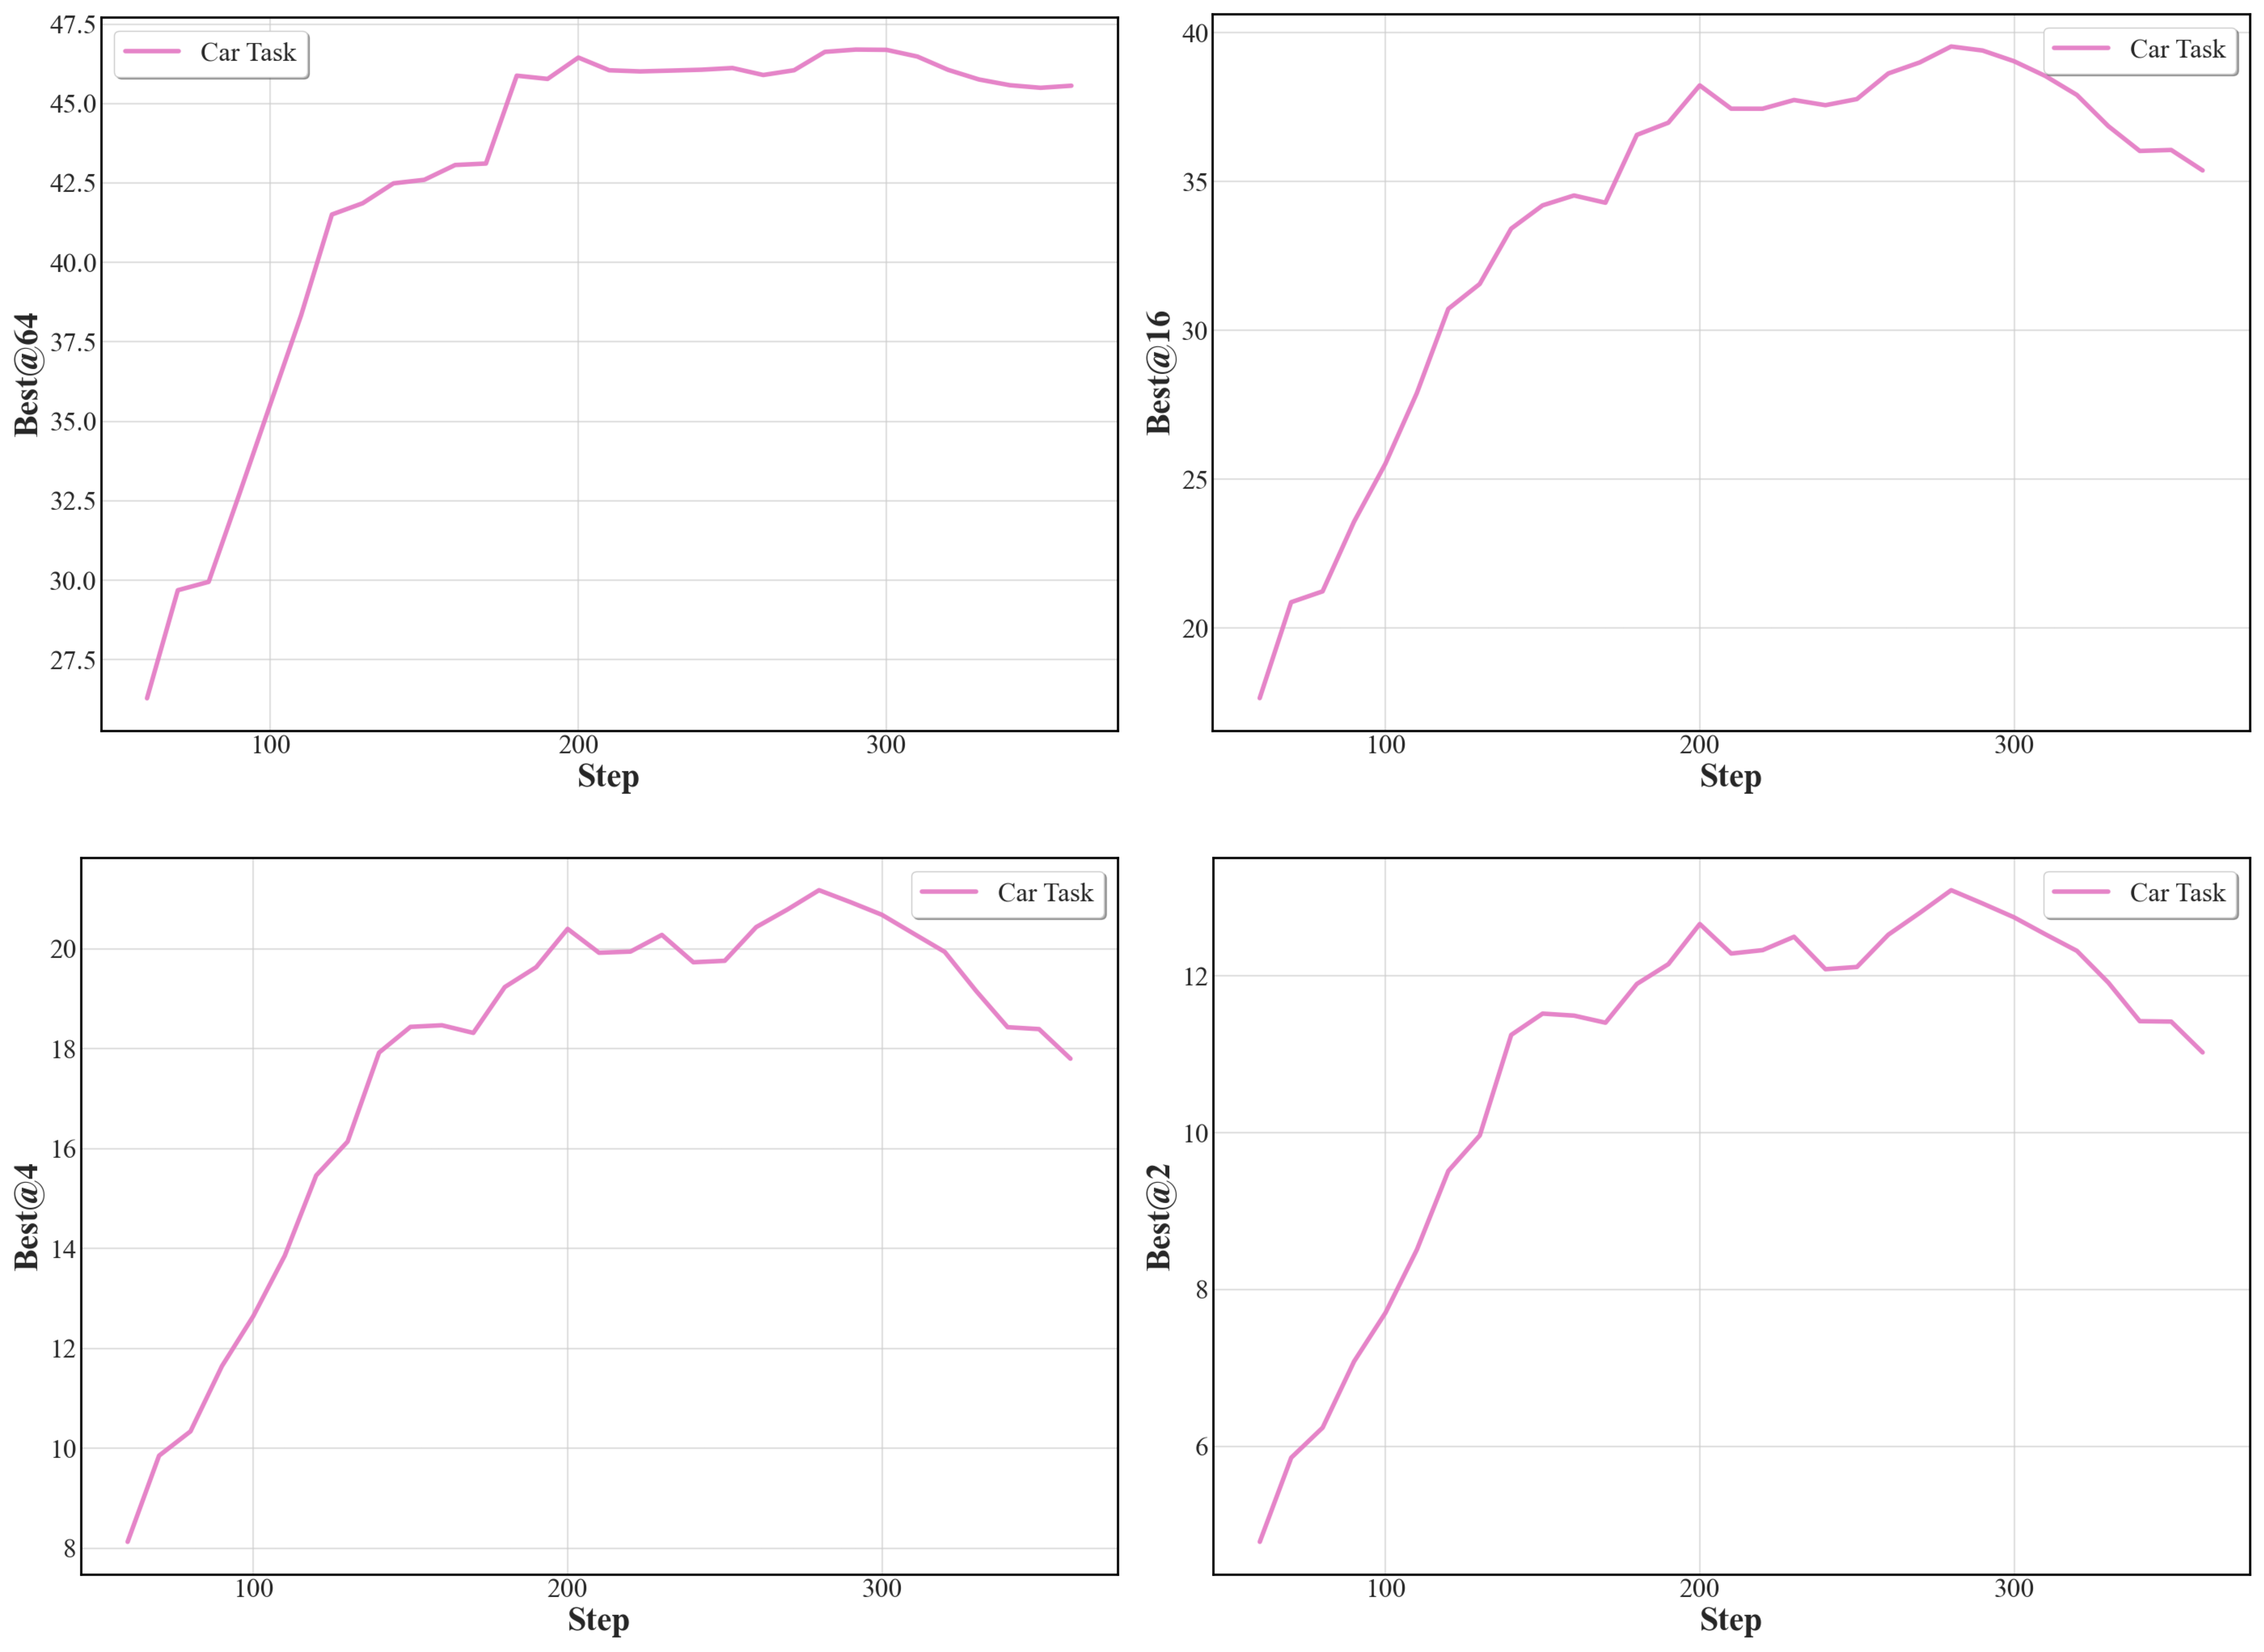
\includegraphics[width=\linewidth]{figures/RL_Metrics/Car/Val_Best.png}
  \caption{\footnotesize \textit{Car task}. Mean Best@N metrics. Similar to the machine validity rate, the Best@N performance increases quickly and remains stable in rest training periods.}\label{fig:RL-car-best@n}
\end{figure}


\clearpage
\newpage
\section{Generated Samples}

\subsection{From RL-finetuned Models}
Here, we present some of the best RL samples from rollouts, as well as examples from the agentic workflow. Fig.~\ref{fig:RL_best_sample} displays the RL rollout samples, while Fig.~\ref{fig:test_time_scaling_gallery} illustrates the agentic workflow samples. 

\begin{figure}[h!]
  \centering
  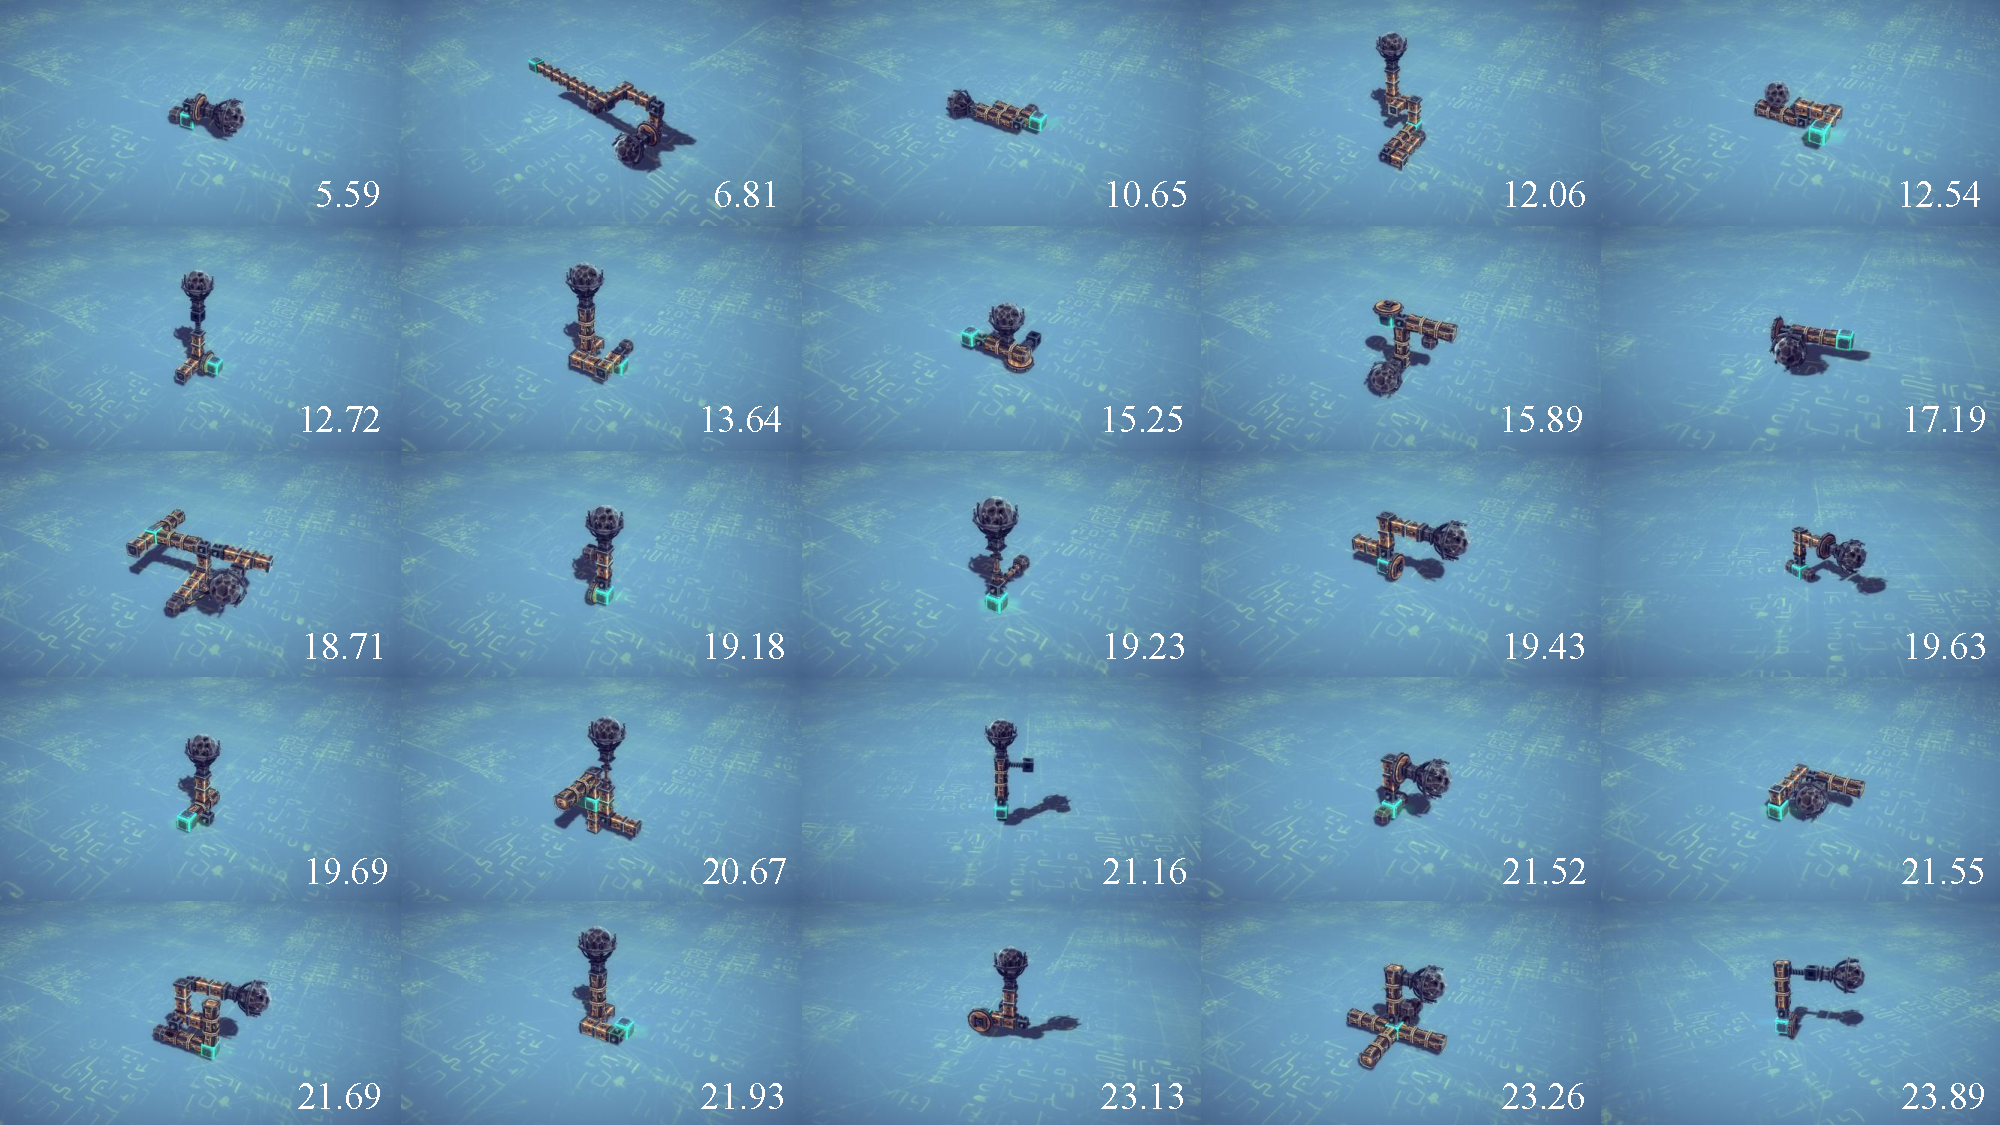
\includegraphics[width=\linewidth]{figures/RL_sample_new_v2.pdf}
  \caption{\footnotesize Qwen2.5-14B-Instruct cold started RL model \textit{catapult} task sample from roll-out. Throwing distances are labeled on the bottom-right corner of the image.}
  \label{fig:RL_best_sample}
\end{figure}

\newpage
\subsection{From Agentic Workflow}
\begin{figure}[h!]
  \centering
  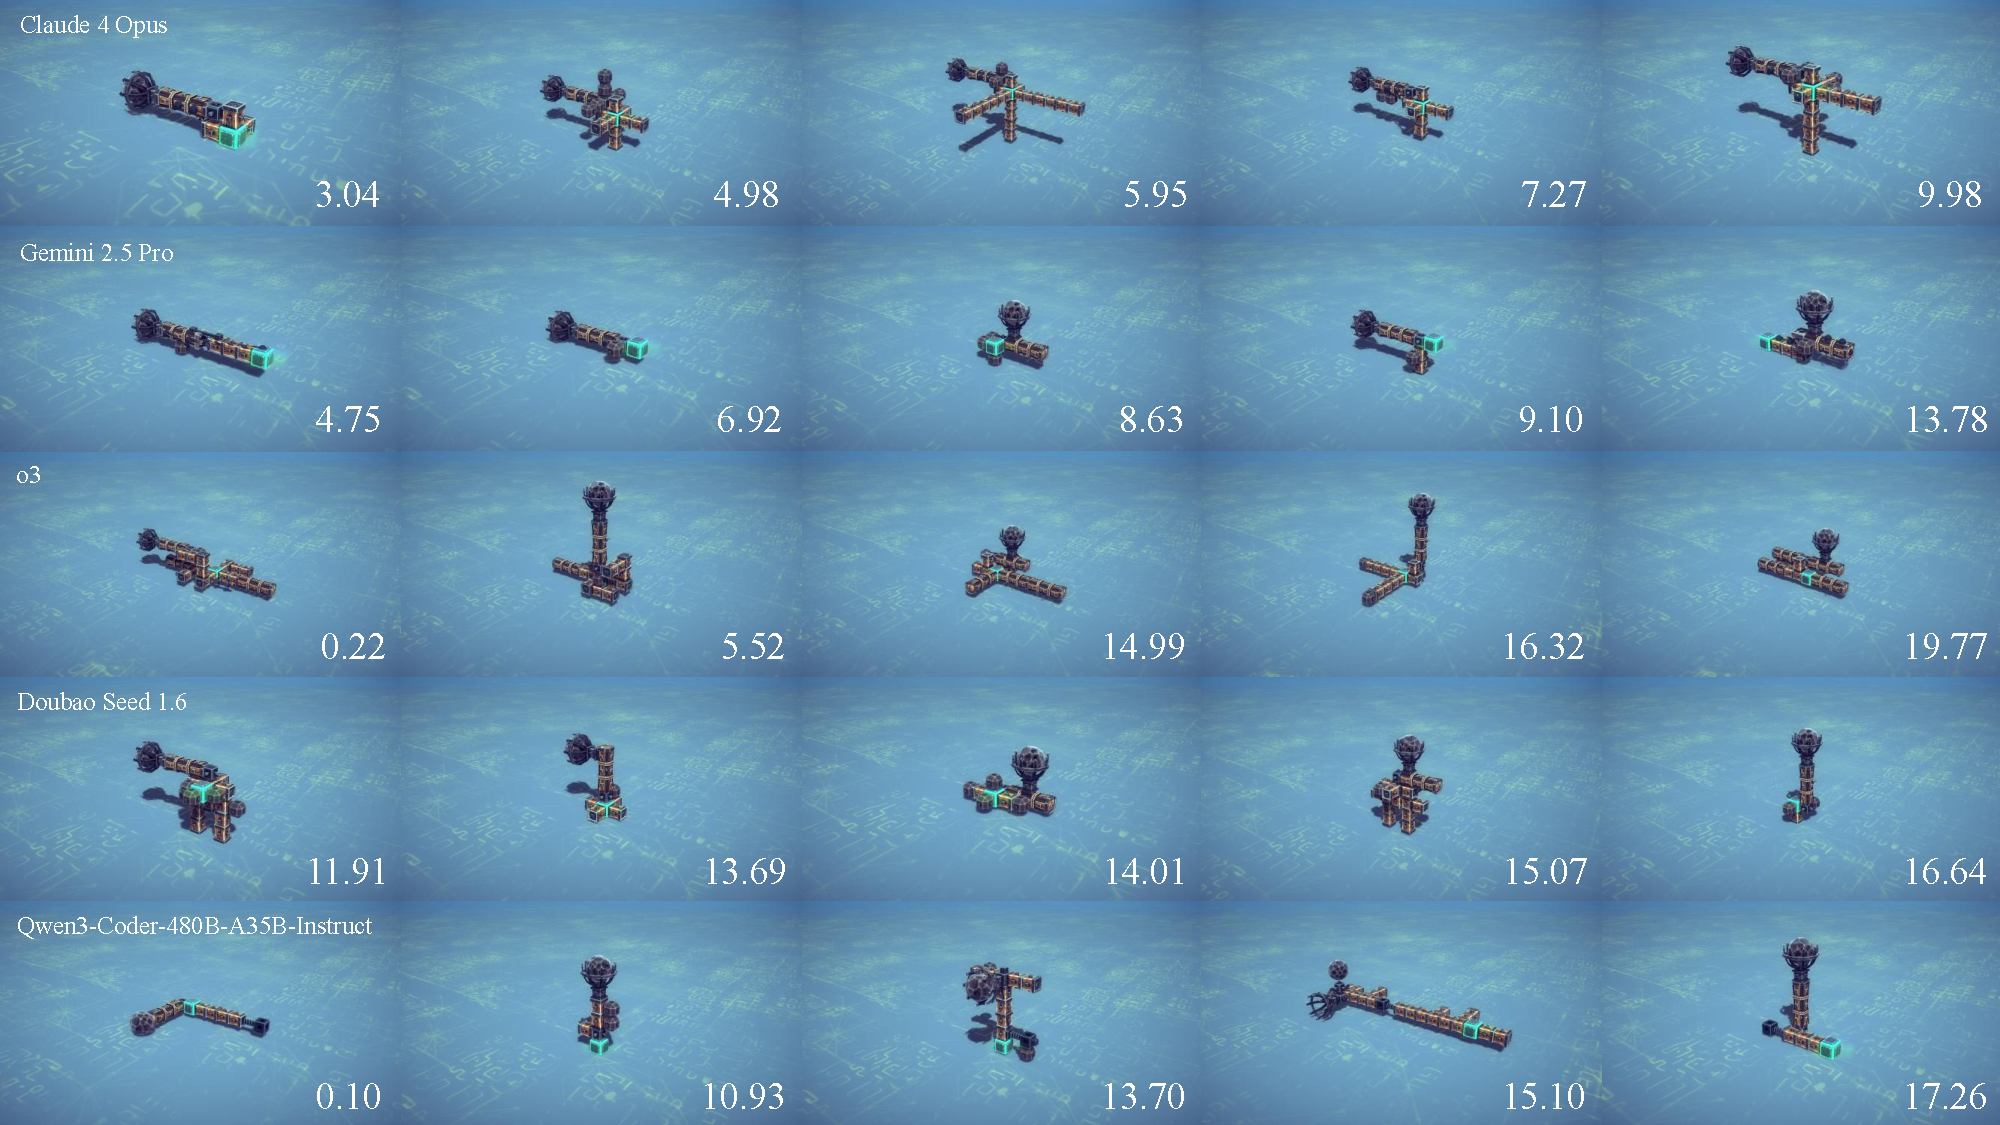
\includegraphics[width=\linewidth]{figures/test_time_scaling_gallery_withcaption.pdf}
  \caption{\footnotesize The LLM inference gallery of machine-generated samples. The rows, from top to bottom, were inferred by the following models, respectively: Claude 4 Opus, Gemini 2.5 Pro, o3, Doubao Seed 1.6, and Qwen3-Coder-480B-A35B-Instruct. Throwing distances are labeled on the bottom-right corner of the image.}
  \label{fig:test_time_scaling_gallery}
\end{figure}


\clearpage
\newpage
\section{Relations between CoT and Machines}



To further investigate if high-level machine blueprint or low-level part placement is more important, 
we experiment with machine generation of LLMs by generating machine details conditioned on Gemini-generated CoT (instead of on CoT produced by themselves). 
We find that with Gemini CoT, almost all LLMs design machines that are more visually similar to "catapults", as shown in Fig.~\ref{fig:LLM-feed-gemini-cot}. We therefore hypothesize that the major gap between other LLMs, especially open-source ones, and Gemini 2.5 Pro is the abstract-level spatial and physics reasoning on machine designs.


\begin{figure}[h!]
  \centering
  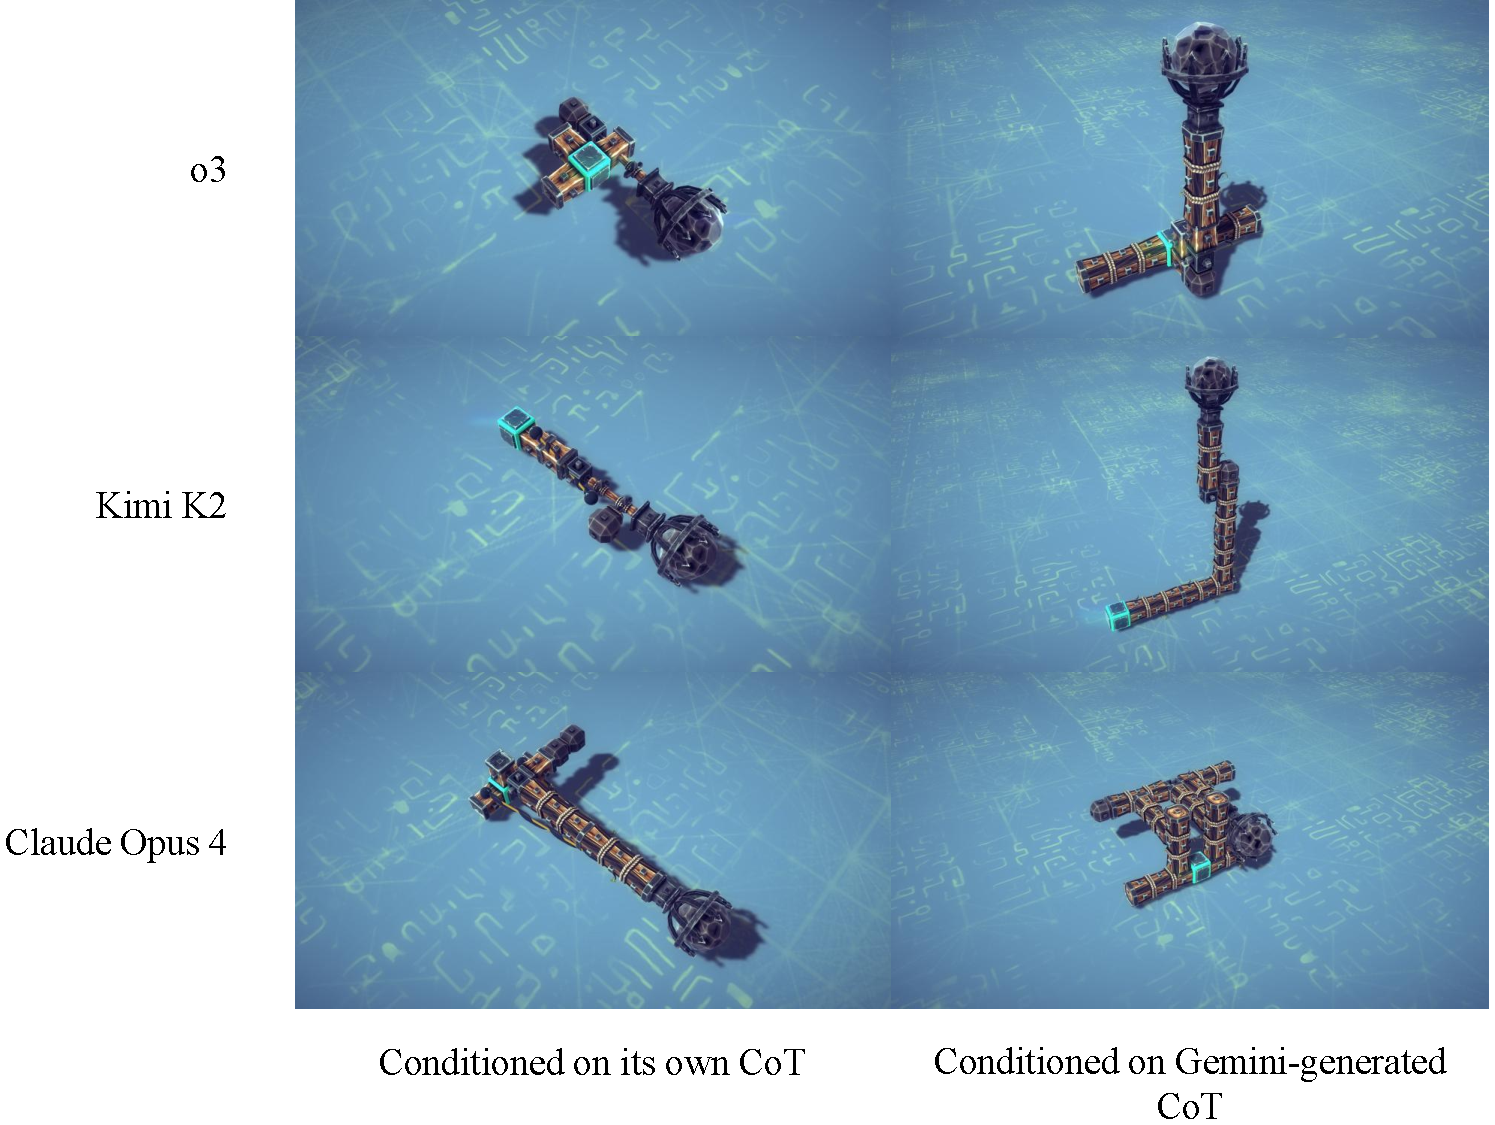
\includegraphics[width=\linewidth]{figures/LLM_feed_gemini_cot_v4_cropped.pdf}
  \caption{\footnotesize Comparison between generated machines conditioned on their own CoT or Gemini-generated CoT.}
  \label{fig:LLM-feed-gemini-cot}
\end{figure}

\clearpage
\newpage
\section{CoT Samples from Gemini 2.5 Pro}
\subsection{Single Agent}
\begin{lstlisting}
system:
<System Prompt>
user:
Design a machine to throw a boulder (type id 36) in a parabolic trajectory. You must use exactly one boulder. Optimize for throw distance, height, and speed. Apply the principle of leverage correctly, balancing the weight of the projectile.

assistant:
<think>
**Analyzing Catapult Components**
I'm now building a catapult with a rigid frame using `Wooden Block`s to ensure stability. I plan to use a `Log` as the throwing arm, attached to a constructed pivot point. The `Container` will hold the boulder at the arm's end.

**Devising Launch Mechanisms**
I'm reconsidering my approach. With the provided constraints, a trebuchet is out. The single boulder and lack of hinges necessitate a catapult. I must leverage the `Rubber Band`. My plan is to design a tension-based catapult for the boulder, prioritizing stability and throwing arm efficiency.

**Optimizing for Distance**
I'm now focused on the tension-powered catapult. My plan is for a solid base, a pivot, a lever arm, a boulder-holding container, and rubber bands. I'm working on the arm's length and the positioning of the rubber bands for maximum launch power and the best trajectory for the boulder.

**Assessing the Lever Arm**
I'm now working on the arm, crucial for force. I must decide on its length and how it attaches to the pivot. I'm considering different attachment methods to create a stable but rotatable lever, exploring options for maximum launch power and height.

**Evaluating Construction Strategies**
I'm stuck! I need to use a catapult given the constraints. But, the lack of a hinge restricts my options. I'm exploring different ways to connect the throwing arm to the frame and leverage the `Rubber Band` for propulsion.

**Designing a Hybrid Catapult**
I've sketched out the structure, pivoting on the `Rotating Block`, with a base and uprights. The throwing arm will comprise a `Log`, with a `Container` at the tip. I am struggling with the rubber band attachment. I will have to ensure the right angles and tension.

**Evaluating Rubber Band Placement**
I'm now focusing on the final adjustments. With the core design finalized, the key is the `Rubber Band` placement. The goal is maximizing launch power by carefully considering the band's attachment points and the angle of force application. I aim to achieve a long throw with this arrangement.

**Evaluating Lever Arm Placement**
I'm now focused on the throwing arm's construction and its link to the rotating pivot. I've built the base and the pivot structure. The lever arm's length and the location for the `Container` are my next priorities. The rubber band attachments also need to be evaluated.

**Engineering the Launch Mechanism**
I'm now focused on a tension-based catapult. It's time to build, starting with a solid base and a stable pivot point using the `Rotating Block`. My priorities are a strong throwing arm, the right `Container` for the boulder, and, critically, the strategic placement of the `Rubber Band`s.

**Refining the Design**
I'm now focused on the core catapult design. The need for a simple build, given the constraints, favors a straightforward tension catapult. I am planning a solid base, a lever arm (most likely a `Log`), a container for the boulder, and the crucial application of `Rubber Band`s to generate the launch force.

**Finalizing Catapult Design**
I've spent time analyzing the limitations and refining the catapult build. I've now decided on the layout. The catapult will be built around a sturdy frame, a pivot using a `Rotating Block`, an arm (lever), and the utilization of the `Rubber Band` for propulsion. I am ready for the final assembly.

**Constructing the Base**
I'm now focused on the basic frame. I've decided to construct it from logs for stability. The goal is a sturdy structure to anchor the catapult's components, primarily the `Rotating Block` and lever arm. I'm focusing on the geometry.

**Analyzing Leverage Application**
I'm now focused on catapult design. Given the one-boulder rule and lack of hinges, I'll focus on a lever-based catapult. I am now determining the lever arm length.

**Building a Lever Catapult**
I'm planning a basic tension-based catapult using the `Rotating Block` as a pivot. I'm focusing on the throwing arm's dimensions, the `Rubber Band` placement to maximize launch power, and the `Container` block to hold the boulder.

**Constructing Launch Support**
I'm now focused on the basic design. With the user's need to launch a single boulder, a tension-based catapult is optimal. I'll build it around the `Rotating Block`. I'm using a `Log` for the arm and planning a base, rubber band connections, and the boulder's container.

**Planning the Build**
I'm streamlining the design. The key will be a stable base, a `Rotating Block` for the pivot, and a lever arm. I'll use a `Container` to hold the boulder, and the `Rubber Band`s will be the power source. Now I am evaluating the dimensions and the best placement of each part.

**Constructing the Launching Mechanism**
I'm designing a simplified catapult, keeping the focus on its functionality and the user's requirement for a single boulder and the available blocks. I plan to use a `Rotating Block` as the pivot. The rest of the design must center around this `Rotating Block` component.

**Constructing the Catapult**
I've established the foundation of the catapult, focusing on a solid base and pivot mechanism. The challenge now is to construct the lever arm and connect it effectively to the `Rotating Block`, while also determining how to hold the boulder. I will prioritize a design maximizing force transfer for launch.

**Constructing a Lever Arm**
I'm solidifying the basic build: a catapult, powered by rubber bands, given the constraints. The next step is constructing the lever arm, deciding its dimensions and how it will attach to the pivot point for optimal force transfer.

**Constructing the Final Catapult**
I've finalized the construction plan. The tension-based catapult, using the `Rotating Block` for the pivot and a lever arm, is my focus. I will use a `Container` for the boulder, and the `Rubber Band` for launching, paying close attention to force application and frame design.

**Outlining Catapult Construction**
I've sketched out the build, focusing on a tension-powered catapult. A base, a pivoting lever arm, and a boulder holder are planned. My design will depend on a stable foundation and the proper application of rubber bands for generating enough force for distance and height.

**Constructing the Catapult**
I've arrived at a straightforward plan for a tension-powered catapult, using the available blocks. I'm focusing on a design to maximize launch potential. The base, pivot point, arm, and rubber bands will be the key components for an efficient, functional build.

**Devising the Final Catapult**
I've finalized the core design. I am now sure of a tension-based catapult; the concept is simple and effective. My focus is now on the construction idea and creating the blocks. I am convinced it will be a simple build and the machine can leverage the `Rotating Block` and `Rubber Band` to meet the user's launch goals.

**Constructing a Launching System**
I'm finalizing the blueprint now. The tension-based catapult will use a base, a pivot with the `Rotating Block`, and a lever arm for the boulder. I'll ensure maximum launch power through strategic rubber band placement and precise measurements. I need a strong yet streamlined design.

**Constructing a Functional Catapult**
I've finalized the plan. The design uses a tension-based catapult, with a "Rotating Block" for a pivot. A sturdy base with two Log arms ensures stability, while two Rubber Bands generate the launch force. The boulder holder is a "Container", and the system prioritizes lever arm efficiency for maximum height and distance.

**Formulating Final Design**
I'm now certain: a tension-based catapult, incorporating the `Rotating Block` for the pivot, will meet the user's needs. The goal is maximum launch power within the given constraints. I'll sketch out the construction, outlining the key blocks and how they fit together. I've a solid plan.

Construction Idea:
I will design a tension-powered catapult to launch the boulder. The design prioritizes a long throwing distance and height by utilizing a long lever arm.

The machine has four main parts:
1.  **Base Frame:** A T-shaped base, constructed from a central 'Wooden Block' and two 'Log's extending sideways, provides a wide, stable footprint to handle the throwing forces and prevent the machine from tipping over.
2.  **Support Tower:** Two 'Log's rise vertically from the ends of the base, creating a tall, sturdy support structure for the pivot axle.
3.  **Lever Arm Assembly:** This is the core of the catapult. A 'Rotating Block' is used as a functional hinge/axle, mounted on one of the support uprights. A 'Small Wooden Block' acts as a hub on this axle, with a long 'Log' attached pointing up (the throwing arm) and a 'Small Wooden Block' attached pointing down (the short lever). This structure creates the necessary leverage. At the end of the throwing arm, a 'Container' is mounted via an adapter block to hold the 'Boulder'.
4.  **Power System:** Two 'Rubber Band' blocks provide the propulsive force. They connect from a forward-projecting 'Log' on the base to the short lever arm. The stretched rubber bands contract rapidly, pulling the short arm down and forward, which in turn whips the long throwing arm upwards and forwards, launching the boulder in a high parabolic trajectory.

This design maximizes the lever ratio to achieve high velocity for the projectile, while the robust frame maintains stability during the launch.

necessary_blocks ```[1, 63, 22, 15, 30, 36, 9]```
</think>

JSON:
```json
[
{"type": 0, "id": 0, "parent": -1, "face_id": -1}
{"type": 1, "id": 1, "parent": 0, "face_id": 1}
{"type": 63, "id": 2, "parent": 1, "face_id": 1}
{"type": 63, "id": 3, "parent": 1, "face_id": 3}
{"type": 63, "id": 4, "parent": 2, "face_id": 6}
{"type": 63, "id": 5, "parent": 3, "face_id": 6}
{"type": 22, "id": 6, "parent": 4, "face_id": 4}
{"type": 15, "id": 7, "parent": 6, "face_id": 3}
{"type": 63, "id": 8, "parent": 7, "face_id": 3}
{"type": 15, "id": 9, "parent": 7, "face_id": 4}
{"type": 15, "id": 10, "parent": 8, "face_id": 0}
{"type": 30, "id": 11, "parent": 10, "face_id": 3}
{"type": 36, "id": 12, "parent": 11, "face_id": 0}
{"type": 63, "id": 13, "parent": 0, "face_id": 0}
{"type": 9, "id": 14, "parent_a": 13, "face_id_a": 1, "parent_b": 9, "face_id_b": 1}
{"type": 9, "id": 15, "parent_a": 13, "face_id_a": 3, "parent_b": 9, "face_id_b": 2}
]
```
\end{lstlisting}

\subsection{Meta Designer}
\begin{lstlisting}
system:
<System Prompt>

user:
Design a machine to throw a boulder (type id 36) in a parabolic
trajectory. You must use exactly one boulder. Optimize for throw distance
, height, and speed. Apply the principle of leverage correctly, balancing
the weight of the projectile.

meta-designer output:
```json
{
    "definition": "Construct a machine that can throw boulders in a parabolic trajectory, designed to maximize throw distance and height by utilizing the principle of leverage.",
    "function_points": [
        "Establish a stable foundation to withstand recoil and prevent tipping.",
        "Implement a powered lever arm for projectile propulsion.",
        "Carry and release a boulder projectile at the apex of the arm's swing."
    ],
    "design_structure": [
        {
            "function_name": "Base and Support Frame",
            "description": "A wide, static frame built from the Start Block. It provides stability for the machine and includes a vertical support to mount the rotating mechanism, as well as a stop block to halt the throwing arm's motion.",
            "related_function_points": [
                "Establish a stable foundation to withstand recoil and prevent tipping."
            ]
        },
        {
            "function_name": "Powered Throwing Arm",
            "description": "A composite structure consisting of a powered pivot, a long lever arm, and a projectile holder. The Rotating Block provides rapid rotational force, the Log acts as the lever to amplify speed, and the Container holds the Boulder, releasing it via inertia.",
            "related_function_points": [
                "Implement a powered lever arm for projectile propulsion.",
                "Carry and release a boulder projectile at the apex of the arm's swing."
            ]
        }
    ],
    "build_order": [
        "Base and Support Frame",
        "Powered Throwing Arm"
    ],
    "machine_structure": {
        "Base and Support Frame": {
            "type": [
                1,
                15
            ],
            "guidance": "Wooden Blocks (ID 1) and Small Wooden Blocks (ID 15) are used to build a wide, heavy base that prevents tipping. They also form a tower to elevate the pivot point and a physical stop to arrest the arm's rotation, which is crucial for the release mechanism."
        },
        "Powered Throwing Arm": {
            "type": [
                22,
                63,
                30,
                36
            ],
            "guidance": "A Rotating Block (ID 22) provides the high-speed rotational power. This is attached to a Log (ID 63), which acts as a long, robust lever arm. A Container (ID 30) is placed at the end of the arm to hold the Boulder (ID 36) projectile."
        }
    }
}
```

\end{lstlisting}


\subsection{Designer}
\begin{lstlisting}
system:
<System Prompt>

designer-layer1 input:
On the basis of the existing structure, generate [Base and Support Frame], [A wide, static frame built from the Start Block. It provides stability for the machine and includes a vertical support to mount the rotating mechanism, as well as a stop block to halt the throwing arm's motion.], as ['Establish a stable foundation to withstand recoil and prevent tipping.'], using block type[1, 15], [Wooden Blocks (ID 1) and Small Wooden Blocks (ID 15) are used to build a wide, heavy base that prevents tipping. They also form a tower to elevate the pivot point and a physical stop to arrest the arm's rotation, which is crucial for the release mechanism.]

designer-output-layer1:
Based on the existing structure, a Base and Support Frame was generated to establish a stable foundation to withstand recoil and prevent tipping. Ultimately, the block types [1, 15] were decided upon. No blocks were removed as they were all suitable for the design.
JSON:
```json
[
{"type": "0", "id": 0, "parent": -1, "face_id": -1}
{"type": "1", "id": 1, "parent": 0, "face_id": 1}
{"type": "1", "id": 2, "parent": 0, "face_id": 2}
{"type": "1", "id": 3, "parent": 0, "face_id": 0}
{"type": "1", "id": 4, "parent": 1, "face_id": 2}
{"type": "1", "id": 5, "parent": 2, "face_id": 4}
{"type": "1", "id": 6, "parent": 0, "face_id": 3}
{"type": "1", "id": 7, "parent": 6, "face_id": 6}
{"type": "1", "id": 8, "parent": 7, "face_id": 6}
{"type": "15", "id": 9, "parent": 8, "face_id": 0}
]
```

designer-layer2:
On the basis of the existing structure, generate [Powered Throwing Arm], [A composite structure consisting of a powered pivot, a long lever arm, and a projectile holder. The Rotating Block provides rapid rotational force, the Log acts as the lever to amplify speed, and the Container holds the Boulder, releasing it via inertia.], as ['Implement a powered lever arm for projectile propulsion.', "Carry and release a boulder projectile at the apex of the arm's swing."], using block type [22, 63, 30, 36], [A Rotating Block (ID 22) provides the high-speed rotational power. This is attached to a Log (ID 63), which acts as a long, robust lever arm. A Container (ID 30) is placed at the end of the arm to hold the Boulder (ID 36) projectile.]
<3D Info>

designer-output-layer2:
Based on the existing structure, a Powered Throwing Arm was generated as Implement a powered lever arm for projectile propulsion.,Carry and release a boulder projectile at the apex of the arm's swing.. 
Ultimately, the block types [22, 63, 30, 36] were decided upon, while [] were removed due to [].
JSON:
```json
[
  {"type": "0", "id": 0, "parent": -1, "face_id": -1},
  {"type": "1", "id": 1, "parent": 0, "face_id": 1},
  {"type": "1", "id": 2, "parent": 0, "face_id": 2},
  {"type": "1", "id": 3, "parent": 0, "face_id": 0},
  {"type": "1", "id": 4, "parent": 1, "face_id": 2},
  {"type": "1", "id": 5, "parent": 2, "face_id": 4},
  {"type": "1", "id": 6, "parent": 0, "face_id": 3},
  {"type": "1", "id": 7, "parent": 6, "face_id": 6},
  {"type": "1", "id": 8, "parent": 7, "face_id": 6},
  {"type": "15", "id": 9, "parent": 8, "face_id": 0},
  {"type": "22", "id": 10, "parent": 8, "face_id": 4},
  {"type": "63", "id": 11, "parent": 10, "face_id": 3},
  {"type": "30", "id": 12, "parent": 11, "face_id": 0},
  {"type": "36", "id": 13, "parent": 12, "face_id": 0}
]
```
\end{lstlisting}

\subsection{Inspector}
\begin{lstlisting}
system:
<System Prompt>

inspector input:
Task Introduction

Construct a machine that can throw boulders in a parabolic trajectory, designed to maximize throw distance and height by utilizing the principle of leverage.

JSON Information
<JSON>

3D Information
<3D Information>

Questions
<Inspector Questions>

inspector-output:
<Three-Dimensional Perception of the World>
{
    "Coordinate System": "Left-Handed System",
    "Up": "y",
    "Right": "x",
    "Forward": "z",
    "Frontmost Block": {"3": [0.0, 0.0, 1.5]},
    "Rearmost Block": {"9": [2.0, 2.0, -3.0]},
    "Leftmost Block": {"5": [-2.0, 0.0, 1.5]},
    "Rightmost Block": {"7": [2.0, 1.5, 0.0]},
    "Topmost Block": {"13": [1.0, 7.4, -2.0]},
    "Lowest Block": {"0": [0, 0, 0]}
}
</Three-Dimensional Perception of the World>

<Question Answer>
1.  **Dynamic Blocks Analysis:**
    The only dynamic block in this machine is the `Rotating Block` [10].
    *   **Position and Orientation**: The `Rotating Block` [10] is located at center coordinates [1.0, 2.0, -2.0] with a global orientation of 'x-'.
    *   **Analysis**:
        a. **Impact on the machine**: The `Rotating Block` [10] serves as the pivot for the throwing arm. It is the core component intended to generate the throwing motion.
        b. **Direction of force**: The block is oriented along the 'x-' axis, meaning its rotation axis is the global x-axis. When activated, it will generate a torque, causing its sub-blocks to rotate in the y-z plane.
        c. **Impact on sub-blocks and machine**: The `Rotating Block` [10] will cause its child blocks ([11], [12], [13]) to swing upwards and forwards in a powerful arc. Simultaneously, it will exert an equal and opposite reaction torque on its parent block [8] and the entire support structure, which will likely cause the machine to violently tip over or break.

2.  **Special Static Blocks Analysis:**
    The special static blocks are the `Container` [12] and the `Boulder` [13].
    *   **Container [12]**: It is located at the end of the throwing arm (`Log` [11]) with its center at [1.0, 6.9, -2.0]. Its orientation is 'y+' (upwards). This placement and orientation are rational, as it correctly positions it to hold the `Boulder` [13] like a cup at the end of the throwing arm.
    *   **Boulder [13]**: It is placed inside the `Container` [12] with its center at [1.0, 7.4, -2.0]. As the projectile, its placement is logical and necessary for the machine's function.

3.  **Balance Check (self-gravity):**
    a. **Center of Gravity**: The calculated center of gravity for the entire machine is approximately at (0.85, 4.22, -1.46). The block closest to this point is the `Log` [11].
    b. **Sinking/Collapse**: Yes, parts of the machine will collapse. The entire throwing mechanism, including the heavy `Boulder` [13] (mass 5), rests on a tall, slender support tower made of single `Wooden Block`s ([6], [7], [8]). This structure is extremely fragile and not braced. The machine is severely top-heavy, and the immense weight concentrated on this single tower will cause it to bend and collapse under gravity alone, even before the `Rotating Block` [10] is activated.

4.  **Comprehensive Analysis:**
    a. **Force Summary**: The primary force is gravity, which makes the top-heavy machine highly unstable due to the high position of the `Boulder` [13]. Upon activation, the `Rotating Block` [10] will generate a massive torque on the throwing arm and an equal reaction torque on the flimsy support tower. The combination of static top-heaviness and dynamic reaction forces will lead to immediate structural failure.
    b. **Logically Unreasonable Blocks**:
        *   **Hierarchical Structure**: `Starting Block` [0] -> `Wooden Block` [6] -> `Wooden Block` [7] -> `Wooden Block` [8].
        *   **Reason for Unreasonableness**: The support tower consisting of blocks [6], [7], and [8] is fundamentally flawed. It is a single, unbraced column tasked with supporting the entire throwing arm and the heavy `Boulder` [13]. This design is far too weak to handle the static weight, let alone the powerful dynamic forces and reaction torque from the `Rotating Block` [10]. The machine is guaranteed to collapse.
</Question Answer>

<Summary of Design Defects>
1. Problem description, involving blocks: [6, 7, 8], belonging to structure: "Base and Support Frame"
   The support tower for the throwing mechanism, composed of blocks [6], [7], and [8], is critically weak. It is a single, unbraced column made of wooden blocks, which is completely inadequate to support the massive weight of the throwing arm and the `Boulder` [13]. The structure will collapse under its own weight or instantly shatter upon activation of the `Rotating Block` [10] due to the immense reaction torque.
</Summary of Design Defects>
\end{lstlisting}

\subsection{Environment Querier}
\begin{lstlisting}
system:
<System Prompt>

environment-querier input:
Task Introduction
Construct a machine that can throw boulders in a parabolic trajectory, designed to maximize throw distance and height by utilizing the principle of leverage.

Mechanical JSON Structure
<JSON>

3D Information
<3D Information>

Environment Feedback
machine damaged:
    machine parts
        DoubleWoodenBlock order_id:8 occurred at 0.4 sec block order_id 13 
boulder throwing distance 5.63
boulder max height 7.3
boulder actual position in first 5 seconds
[1.0, 7.01, -1.5], [0.84, 7.34, -2.44], [0.64, 5.69, -6.2], [0.61, 3.28, -9.97], [0.57, 1.68, -10.14], [0.38, 1.78, -9.45], [0.17, 1.72, -8.76], [-0.03, 1.52, -8.13], [-0.22, 1.22, -7.61], [-0.36, 0.85, -7.23], [-0.47, 0.48, -6.98], [-0.53, 0.16, -6.86], [-0.55, -0.07, -6.83], [-0.55, -0.18, -6.87], [-0.53, -0.17, -6.92], [-0.52, -0.03, -6.94], [-0.52, 0.21, -6.9], [-0.55, 0.51, -6.76], [-0.6, 0.85, -6.52], [-0.69, 1.18, -6.16], [-0.81, 1.45, -5.72], [-0.95, 1.66, -5.2], [-1.11, 1.76, -4.64], [-1.28, 1.76, -4.07], [-1.44, 1.66, -3.53]

environment-querier-output:
<Thought Process>
The user wants me to analyze a boulder-throwing machine that is failing its task.

**1. Analyze the Task and Machine Design:**
*   **Objective:** Build a leverage-based machine to throw a boulder for maximum distance and height. This implies a catapult or trebuchet design.
*   **Machine Structure:**
    *   **Base:** A wide base is constructed using `Wooden Block`s (ID 1, 2, 3, 4, 5, 6) connected to the `Starting Block` (ID 0). This seems designed for stability.
    *   **Tower:** A vertical tower is built on the right side of the base with `Wooden Block`s (ID 6, 7, 8). Block 8 is the apex of this support structure.
    *   **Lever Arm:** A `Rotating Block` (ID 10) is mounted on top of the tower (on block 8), serving as the fulcrum. A `Log` (ID 11) acts as the throwing arm, with a `Container` (ID 12) and `Boulder` (ID 13) at the top. A `Ballast` (ID 14) is attached to the other side of the `Rotating Block` as a counterweight.
    *   **Power System:** The machine uses a combination of a powered `Rotating Block` (ID 10) and two `Rubber Band`s (ID 15, 16). The rubber bands connect the top of the tower (block 8) to points on the base (blocks 3 and 5).

**2. Analyze the Environmental Feedback:**
*   **`machine damaged`**: This is the most critical piece of feedback. The machine is breaking during operation.
*   **`machine parts: DoubleWoodenBlock order_id:8`**: The failure point is identified as block 8. This is the `Wooden Block` that supports the entire rotating lever arm assembly.
*   **`occurred at 0.4sec`**: The failure is almost instantaneous, indicating a massive, immediate overload on the structure.
*   **Boulder Performance:** The boulder travels a mere 5.63 units and ends up behind its starting Z coordinate. This confirms a catastrophic failure of the launch mechanism, not just a weak throw. The arm is likely collapsing or swinging backward.

**3. Synthesize and Hypothesize the Root Cause:**
*   The point of failure (block 8) is subjected to several immense forces:
    1.  **Static Load:** The weight of the entire lever arm assembly (rotating block, log, container, boulder, ballast) rests on it.
    2.  **Dynamic Load:** The torque from the `Rotating Block` (ID 10) creates a powerful reaction force on its mount point (block 8).
    3.  **Tension Load:** The two `Rubber Band`s (ID 15, 16) are stretched from block 8 down to the base. When the simulation starts, they will contract with immense force, pulling down and forward on block 8.
*   **Hypothesis:** The combination of these forces, particularly the sudden, immense tension from the rubber bands, is causing block 8 to shear off from the rest of the tower (block 7). The tower itself, being a single column of wooden blocks, is structurally weak and cannot withstand this combination of bending and shear stress. The rubber bands are incorrectly placed; instead of powering the lever arm, they are destroying the support structure. The machine is literally tearing itself apart.

**4. Formulate a Plan for Further Investigation:**
To confirm this hypothesis, I need to observe the behavior of the key components involved in the structural failure around the time of the collapse (0.4s).

*   **Block 8 (Failure Point):** I need to see its position and rotation to confirm it's being ripped from its mounting.
*   **Block 10 (Rotating Block/Fulcrum):** Its movement will show the forces being applied by the lever arm onto block 8.
*   **Block 11 (Lever Arm):** Its motion will confirm the direction of the attempted throw and the overall collapse dynamics.
*   **Rubber Bands (15 & 16):** I need to check their `length` property. A rapid decrease in length will prove they are contracting and applying the destructive force I suspect.

Based on this analysis, I will request detailed feedback on these specific components to verify the cause of the failure.
</Thought Process>
<Required Feedback>
[
    {
        "id": 8,
        "duration": [0.0, 0.8],
        "properties": ["position", "rotation"]
    },
    {
        "id": 10,
        "duration": [0.0, 0.8],
        "properties": ["position", "rotation"]
    },
    {
        "id": 11,
        "duration": [0.0, 0.8],
        "properties": ["position", "rotation"]
    },
    {
        "id": 15,
        "duration": [0.0, 0.8],
        "properties": ["length"]
    },
    {
        "id": 16,
        "duration": [0.0, 0.8],
        "properties": ["length"]
    }
]
</Required Feedback>
\end{lstlisting}

\subsection{Refiner}
\begin{lstlisting}
system:
<System Prompt>

refiner input:
Task Introduction
Construct a machine that can throw boulders in a parabolic trajectory, designed to maximize throw distance and height by utilizing the principle of leverage.

Mechanical JSON Structure
<JSON>

3D Information
<3D Information>

Environment Feedback
machine damaged:
    machine parts
        DoubleWoodenBlock order_id:8 occurred at 0.4 sec block order_id 13 
boulder throwing distance 5.63
boulder max height 7.3
boulder actual position in first 5 seconds
[1.0, 7.01, -1.5], [0.84, 7.34, -2.44], [0.64, 5.69, -6.2], [0.61, 3.28, -9.97], [0.57, 1.68, -10.14], [0.38, 1.78, -9.45], [0.17, 1.72, -8.76], [-0.03, 1.52, -8.13], [-0.22, 1.22, -7.61], [-0.36, 0.85, -7.23], [-0.47, 0.48, -6.98], [-0.53, 0.16, -6.86], [-0.55, -0.07, -6.83], [-0.55, -0.18, -6.87], [-0.53, -0.17, -6.92], [-0.52, -0.03, -6.94], [-0.52, 0.21, -6.9], [-0.55, 0.51, -6.76], [-0.6, 0.85, -6.52], [-0.69, 1.18, -6.16], [-0.81, 1.45, -5.72], [-0.95, 1.66, -5.2], [-1.11, 1.76, -4.64], [-1.28, 1.76, -4.07], [-1.44, 1.66, -3.53]

Querier required feedback
block order_id 8 
    type_id 
        1 
    info duration(s) 
        [0.0, 1.0]
    block broken before below time(s) 
        0.2
    block position 
        [[2.01, 2.49, 0.01]] Due to block broken, the position is incomplete or not recorded
    block velocity
        [[0.15, 1.7, 4.1]] Due to block broken, the velocity is incomplete or not recorded
block order_id 10
    block type_id
        22
    block info duration(s)
        [0.0, 1.0]
    block position
        [[ 1.5 ,  2.52, -1.49], [ 1.5 ,  3.34, -0.56], [1.48, 5.27, 1.08], [0.73, 5.66, 2.42], [0.11, 4.45, 3.64])]
    block rotation
        [[ 0.  , -0.71,  0.01,  0.71], [-0.16, -0.68,  0.18,  0.69], [-0.47, -0.47,  0.51,  0.54], [-0.73, -0.04,  0.08,  0.67], [-0.69,  0.06, -0.04,  0.72]]
block order_id 0
    block type_id 0
    block info duration(s)
        [0.0, 2.0]
    block rotation
        [[0., 0., 0., 1.], [ 0.07,  0.  , -0.01,  1.  ], [ 0.45,  0.06, -0.04,  0.89], [ 0.39,  0.14, -0.09,  0.91], [0.  , 0.15, 0.03, 0.99], [-0.09,  0.05,  0.36,  0.93], [0.2 , 0.01, 0.09, 0.98], [ 0.13, -0.31, -0.13,  0.93], [-0.06, -0.26, -0.1 ,  0.96], [-0.08, -0.18, -0.1 ,  0.97]]

Initial State of the Machine
The machine is initially placed on the ground, facing the z+ direction, with the target direction being z+.
Please remember that the task failure is due to the mechanical design defects. 
Your ultimate goal is to modify the mechanical design defects so that it can complete the task.
The historical modification information represents your previous attempts to make changes, and these steps did not comply with the game rules.
Based on the information about the task failure, please make modifications to the mechanics. 
When designing the modification steps, avoid making the same mistakes as those in the historical modification information.

refiner-output:
<Thought Process>
The user wants me to fix a trebuchet-like machine that is failing.

**1. Analysis of the Machine and Failure:**
*   **Machine Structure:** The machine consists of a base, a vertical tower on the right side, and a rotating arm mounted on top of the tower. The arm has a container with a boulder on one end and was intended to have a counterweight on the other. Power is provided by a `Rotating Block` (ID 10) at the pivot and a `Ballast` (ID 14) acting as a counterweight. Two `Rubber Band`s (ID 15, 16) are connected from the top of the tower (ID 8) to the base, seemingly for stabilization.
*   **Failure Mode:** The simulation feedback consistently reports that `DoubleWoodenBlock id:8` is damaged at 0.4 seconds. Block 8 is the top-most block of the support tower, directly holding the entire rotating assembly (`Rotating Block`, arm, boulder, and ballast).
*   **Root Cause Analysis:**
    *   **Overwhelming Force:** The combination of the `Rotating Block`'s torque and the heavy `Ballast` (ID 14, mass 3) dropping creates an immense rotational force. The `Boulder` (ID 13, mass 5) at the end of a long lever arm (ID 11, `Log`) amplifies this stress. The tower, constructed from simple `Wooden Block`s, cannot withstand this force, leading to the failure of block 8.
    *   **Instability:** The feedback shows the entire machine lifting and tilting (`machine orientation in long time x-`, `machine frequently changes in the following orientations`). This indicates the base is too small and light to counteract the violent motion of the throwing arm. The `Rubber Band`s (ID 15, 16) are connected asymmetrically (from the tower to the front and left parts of the base), which likely introduces a twisting force, contributing to the instability and structural failure rather than preventing it.

**2. Modification Strategy:**
The primary goal is to ensure the machine's structural integrity so it can actually launch the boulder without self-destructing.

*   **Step 1: Reduce Destructive Forces.** The most critical issue is the excessive force breaking block 8. The simplest way to address this is to remove the primary source of this force, the `Ballast` (ID 14). The `Rotating Block` (ID 10) by itself will still provide sufficient power to launch the boulder, but with much less violent acceleration, which the wooden structure should be able to handle.
*   **Step 2: Remove Ineffective Components.** The `Rubber Band`s (ID 15 and 16) are not stabilizing the structure effectively and are likely contributing to the twisting failure due to their asymmetric placement. Removing them will simplify the forces acting on the tower and improve stability.

This plan directly targets the identified points of failure. By removing the ballast and the rubber bands, the stress on the critical component (block 8) is significantly reduced, and the machine's overall stability should improve. The throwing distance might be reduced, but a successful, non-destructive launch is the first priority.

**3. Final Plan:**
1.  Remove `Ballast` (ID 14).
2.  Remove `Rubber Band` (ID 15).
3.  Remove `Rubber Band` (ID 16).

This is a minimal but highly effective set of changes to fix the core problem.
</Thought Process>
<Modification Description>
The machine's support tower (block 8) is breaking due to excessive torque from the ballast and rotating block. The rubber bands are placed asymmetrically, causing twisting forces and instability. I will remove the ballast (ID 14) to reduce the strain on the structure and remove the two rubber bands (ID 15, 16) to eliminate the destabilizing twisting forces.
</Modification Description>
<Simulation Prediction After Modification>
*   **Power Blocks Analysis:** The launch will now be powered solely by the `Rotating Block` (10). The removal of the `Ballast` (14) significantly reduces the peak torque, resulting in a smoother, less violent rotation of the throwing arm. This will prevent the structural failure of the tower.
*   **Balance Check:** Without the heavy ballast dropping and the asymmetric pull from the rubber bands, the machine will be much more stable during operation. The base should remain mostly on the ground, with minimal tipping as the arm swings. The overall center of gravity will be more manageable.
*   **Comprehensive Analysis:** The primary defect, the destruction of block 8, will be resolved. The machine will successfully complete the launch sequence without breaking. While the throwing distance and height may be lower due to the reduced power, the machine will now be functional and can complete its primary task of throwing the boulder.
*   **10-second game simulation prediction:**
    *   **0.0s - 0.5s:** The `Rotating Block` activates, and the arm begins to swing upwards smoothly. The tower (block 8) remains intact.
    *   **0.5s - 1.0s:** The arm reaches its maximum rotation, and the boulder is released from the container. The machine's base remains stable on the ground.
    *   **1.0s - 5.0s:** The boulder travels in a clear parabolic arc. The machine settles without any damage. The final throwing distance will be shorter than the broken attempts but will represent a successful launch.
</Simulation Prediction After Modification>

<Modification Steps>
Remove [14]
Remove [15]
Remove [16]
</Modification Steps>
\end{lstlisting}


\newpage
\section{Single-Agent Prompt}
\label{app:single-agent-prompt}
\begin{lstlisting}
You are a machine builder. Your task is to generate a complete machine as a JSON file based on the user's request. Add new blocks to the initial structure; do not modify or delete it.

I. Rules:
1.  Coordinate System: Left-handed coordinate system, y+ upwards, z+ forward and x+ right.
2.  Block Placement: New blocks must attach to `attachable_faces` of existing blocks. Blocks cannot overlap.
3.  Size Limit: The final machine must not exceed dimensions of 17 (Length, Z), 17 (Width, X), 9.5 (Height, Y).
4.  Functionality: Ensure functional blocks are oriented correctly.
5.  Ground Interaction: The ground automatically conforms to the machine's lowest block. Account for potential collisions between the machine and the ground throughout operation.
6.  Gravity: Every block is subject to gravity; the greater a block's mass, the stronger its downward force. Consider this in your design when the machine is in operation.
7.  Physical rules: Classical mechanical laws such as conservation of momentum are applied.

II. Block Data:
Notes:
You can only use blocks from this list. A block's default orientation is Z+.
1. Attachable face:
   a. `id`: The i-th attachable_face of this block.
   b. `pos`: Coordinates relative to the building center(which is the attachable_face of the parent block) of this block.
   c. `orientation`: Orientation relative to the building center of this block.
2. Tags:
   a. `Non-static`: Block can generate force or movement.
   b. `Non-stable`: Connection to parent is not rigid (e.g., hinges, boulders).
   c. `Linear`: Do not collide with other blocks, but will occupy two attachable_faces.
3. Special Blocks:
   a. Boulder (id 36): Does not physically connect to other blocks.
   b. Spring (id 9): A special block that pulls its two connection points together.

Detailed Infos:
<Block Infos without explanations>

III. JSON Output Format:
1. type: block's type_id
2. id: this is i-th block
3. parent: parent block's id
4. face_id: parent block's constructible_point id
5. Standard Block: `{"type": <int>, "id": <int>, "parent": <int>, "face_id": <int>}`
6. special block (id: 9): `{"type": 9, "id": <int>, "parent_a": <int>, "face_id_a": <int>, "parent_b": <int>, "face_id_b": <int>}`

IV. Final Response Format:
Your response must contain only these two parts:
1. `Chain of thoughts:` 
    a. You need to think step by step, analyse each block's usage, and where to place them. Put your cot in <cot></cot>
    b. `Construction Idea:` A brief explanation of your design, remember to consider necessary block types, note them in ```necessary_blocks [type_1,type_2 ...]```, no more than 300 words.
2.  `JSON:` The complete JSON code inside a ```json ... ``` block. Here is an example: 
```json
    [
        {"type":"0","id":0,"parent":-1,"face_id":-1},
        {"type": <int>, "id": <int>, "parent": <int>, "face_id": <int>},
        ...
    ]
```
\end{lstlisting}


\newpage
\section{Multi-Agent Prompts}
\subsection{Shared Prompts}
\subsubsection{Game Introduction With 3D Knowledge}
\begin{lstlisting}
1. Coordinate System: The game uses a left-handed coordinate system, with the Y-axis pointing upwards. In global coordinates, z+ is forward and x+ is to the right.
2. Construction: New blocks must be connected to the "attachable faces" of existing blocks. The default orientation of blocks is z+.
3. Block Types:
    a. Regular Blocks: Have fixed dimensions and multiple attachable faces.
    b. special blocks (ID 7, 9): Connect two attachable faces, do not collide with other blocks, but will occupy the connection points.
4. Size Limitations: The mechanical dimensions must not exceed Length (z) 17, Width (x) 17  Height (y) 9.5.
\end{lstlisting}

\subsubsection{Machine 3D JSON Format}
\begin{lstlisting}
```json
[
    {"type":"0","id":0,"parent":-1,"face_id":-1},
    {"type":"Block Type ID","id":"Block Order ID","parent":"Parent Block ID","face_id":"Attachable Face ID in Parent Block"},
    ...
]
```
If it is a special block (Type ID is 7 or 9, other blocks are not special blocks), it will be:
```json
{
    "type":"Block Type ID",
    "id":"Block Order ID",
    "parent_a":"Parent A Block Order ID",
    "face_id_a":"Attachable Face ID in Parent A Block",
    "parent_b":"Parent B Block Order ID",
    "face_id_b":"Attachable Face ID in Parent B Block"
}
```
\end{lstlisting}

\subsubsection{Build Guidance}
\begin{lstlisting}
Your task is to: Add new blocks based on the initial machine JSON and construction requirements provided by the user, without deleting the initial structure, and output the final complete JSON.

User Input Format:
1.  Building Objective: Describe the structure and function to be built, and provide a list of recommended block IDs.
2.  Initial JSON: The structural data of the existing machine.

Core Building Rules:
1.  Block Usage: You can only select from the list of recommended block IDs provided by the user. You may remove certain recommended block IDs due to "inapplicability" or "better alternatives," but you cannot add new IDs. If any are removed, the reason must be stated.
2.  Collision Prevention: You must accurately calculate the coordinates and orientation of new blocks based on the orientation and position of the parent block to ensure that the new block does not overlap with the existing structure.
3.  Coordinate System and Orientation: The initial orientation of all blocks is Z+. The final orientation of new blocks must be transformed based on the parent block's orientation and the relative direction of the building point, according to the following rules:
       Oriented z+: Front z+, Back z-, Left x-, Right x+, Up y+, Down y-
       Oriented z-: Front z-, Back z+, Left x+, Right x-, Up y+, Down y-
       Oriented x-: Front x-, Back x+, Left z-, Right z+, Up y+, Down y-
       Oriented x+: Front x+, Back x-, Left z+, Right z-, Up y+, Down y-
       Oriented y+: Front y+, Back y-, Left x-, Right x+, Up z-, Down z+
       Oriented y-: Front y-, Back y+, Left x-, Right x+, Up z+, Down z-

Your Output Format:
1.  Building Plan:
    `Generated [structure summary] to achieve [function]. Finally used blocks [ID1, ID2,...]. Removed [ID3,...] because [reason for removal].`
2.  Final JSON:
    ```json
    [
      // The complete JSON including both the initial structure and the new blocks
    ]
    ```    
\end{lstlisting}

\subsubsection{Meta Designer System Prompt}
\begin{lstlisting}
You are a mechanical designer, and your task is to design a machine in the game Besiege based on the user's requirements. Please gain a general understanding of the game based on the following information:

I. Game Introduction:
1. Besiege is a physics-based construction game developed using Unity. Players need to build various machines to complete different tasks.
2. Besiege only contains basic mechanics and physical laws, such as mass, friction, and collision.
3. Blocks are used to build machines. Each block has its unique functions, advantages, and disadvantages. 

II. Block Introduction:
1. Blocks are mainly divided into five major categories: Basic Blocks, Mobility Blocks, Mechanical Blocks, Weapon Blocks, and Armor Blocks.
- Basic Blocks are the fundamental components of many machines - structural blocks and some basic moving parts.
- Mobility Blocks are primarily designed for movement functions - powered and unpowered wheels, steering blocks, and gears.
- Mechanical Blocks provide various useful auxiliary functions - joints, suspension devices, winches, grabbers, etc.
- Weapon Blocks offer various types of violent output at different ranges - swords and saws for close combat, and cannons and rockets for long-range.
- Armor Blocks can protect the machine from damage or provide useful shapes for carrying other blocks - armor plates and wooden panels, as well as half-pipes and brackets.

2. Here is a detailed introduction to the properties and functions of each block:
| Name | Category | Type ID | Function |
|------|----------|---------|----------|
| Starting Block | Basic | 0 | The Starting Block is the root block of the machine; it is placed at the starting position by default, cannot be moved, cannot be deleted, and only one can exist at a time. |
| Small Wooden Block | Basic | 15 | A basic structural block, cube-shaped, to which other blocks can be attached from any side, making it particularly suitable for constructing the basic framework of machines. |
| Wooden Block | Basic | 1 | A basic mechanical block, twice the length of a Small Wooden Block. |
| Wooden Rod | Basic | 41 | A basic mechanical block, twice the length of a Small Wooden Block, with the same weight as a Wooden Block, but very fragile. |
| Log | Basic | 63 | A basic mechanical block, more robust, three times the length of a Small Wooden Block. |
| Brace | Basic | 7 | A non-placeable block used for reinforcement, built by "attaching" to other blocks, with no collision volume. It is often used to increase the stability of static structures and is not suitable for any dynamic structures. |
| Steering Hinge | Mobility | 28 | The Steering Hinge can rotate blocks along an axis perpendicular to the placement axis. This block can rotate child blocks to a 180-degree direction to the left or right, commonly used for vehicle steering. |
| Steering Block | Mobility | 13 | The Steering Block can rotate blocks along its placement axis, similar to the rotating part of a helicopter's rotor. |
| Powered Wheel | Mobility | 2 | Similar to a car wheel, it can drive itself but cannot turn independently. It is a mechanical device used for moving objects on the ground. |
| Unpowered Wheel | Mobility | 40 | A wheel that does not rotate without external force, otherwise similar to a Powered Wheel. |
| Powered Large Wheel | Mobility | 46 | Similar to a Powered Wheel, but with a radius and thickness twice that of a Powered Wheel. |
| Unpowered Large Wheel | Mobility |  | A wheel that does not rotate without external force, otherwise similar to a Powered Large Wheel. |
| Small Wheel | Mobility | 50 | It works almost the same as a caster wheel (like a shopping cart wheel), unpowered. |
| Universal Joint | Mechanical | 19 | A block that can freely rotate around its placement axis, similar to a Steering Block but without power. |
| Hinge | Mechanical | 5 | Similar to a Steering Hinge, but without power. |
| Ball Joint | Mechanical | 44 | Can swing 360 degrees along the axis perpendicular to the placement axis, but without power. |
| Axle Connector | Mechanical | 76 | Similar to a Ball Joint. |
| Rotating Block | Mechanical | 22 | Powered, it can rotate clockwise or counterclockwise along the axis perpendicular to the placement axis. |
| Suspension | Mechanical | 16 | Shaped like a wooden block, it can buffer forces from all directions. |
| Grabber | Mechanical | 27 | It will grab and hold onto any object it comes into contact with. |
| Spring | Mechanical | 9 | A special block that attaches to two other blocks and can quickly pull them together. Its pulling force is almost entirely dependent on its length. |
| Boulder | Weapon | 36 | A stone that does not directly connect to other blocks even when built on them. It can be used as a projectile weapon and is also commonly used as a target in transportation tests. |
| Elastic Pad | Armor | 87 | Increases the elasticity of the contact surface, providing an effect of rebounding and increasing kinetic energy. |
| Container | Armor | 30 | Can hold child blocks like a bowl, mainly used to carry blocks that cannot be directly connected to the machine. The container has some anti-slip capability, and only one block (the target to be carried) can be placed inside. No other blocks can be added. |
| Roller Wheel | Locomotion | 86 | Similar to the small wheel, but shorter (0.8m). |
|  Grip Pad | Armour | 49 | Block with the highest friction. |
|  Ballast | Flight | 35 | A heavy cubic block used as a counterweight. |

III. Mechanical Design Requirements:
1. When designing the machine, you should adopt a "layered design" approach. Break down the user's requirements into the functions that the machine needs to achieve, and list the functional points.
2. For each functional point, design a structure that can meet the function. A structure can be understood as a "group of blocks," and several structures combined form the machine.
3. For each structure, determine the types of blocks to be used.
4. Determine the construction order of the structures to make the machine-building process layered. List which structure is the foundation and which is the upper-layer structure, and establish the construction sequence chain.

IV. Output Format Requirements:
```json
{
    "definition": "Construct a machine that can fulfill the user's requirements",
    "function_points": ["Function Point 1", "Function Point 2", "Function Point 3"],
    "design_structure": [
        {
            "function_name": "Structure 1 Name",
            "description": "Description of Structure 1",
            "related_function_points": ["Function Point 1", "Function Point 2"]
        },
        {
            "function_name": "Structure 2 Name",
            "description": "Description of Structure 2",
            "related_function_points": ["Function Point 3"]
        }
    ],
    "build_order": ["Structure 2 Name", "Structure 1 Name"],
    "machine_structure": {
        "Structure 1 Name": {
            "block_id": [ID1, ID2, ID3...],
            "guidance": "Guidance here"
        },
        "Structure 2 Name": {
            "block_id": [ID4, ID5, ID6...],
            "guidance": "Guidance here"
        }
    }
}
```
V. Note:
1. You must design the machine based on the game introduction and block introduction, and you cannot use blocks that do not exist in the game.
2. Strictly follow the output format requirements. Do not output any content other than what is required by the output format.
3. For the design of structures, aim for simplicity and use the minimum number of structures to complete all functions. Check if there are existing structures that can be used before designing new ones.
4. When selecting blocks for a structure, limit the types of blocks to no more than three, and preferably use only one type. Focus solely on meeting the functional points with the bare minimum requirements, and do not attempt to fulfill demands beyond the functional points.

I will provide the user input below. Please generate a mechanical overview in JSON format based on the user's description.
\end{lstlisting}


\subsection{Designer System And User Prompt}
\begin{lstlisting}
<system>
You are a mechanical builder in the game "Besiege." 
Your task is to add new blocks to an existing machine structure according to user requests and finally output the complete machine JSON data.
I. Game Introduction:
<Game Introduction With 3D Knowledge>
II. Introduction to Blocks:
<Block Infos>
III. Introduction to JSON Format:
<Machine 3D JSON Format>
IV. Construction Guidance:
<Build Guidance>
V. Output Format Requirements:
Based on the existing structure, a [structural summary] was generated as [functional implementation]. 
Ultimately, the block types [ID1, ID2, ...] were decided upon, while [ID3, ...] were removed due to [reason for removal].
JSON:
```json
...
```
VI. Note:
Building Principles
1. Correct Orientation: Ensure that functional blocks such as wheels and hinges are oriented correctly to achieve the intended function.
2.  Efficiency First:
    a. Complete the design goal with the fewest blocks possible.
    b. The ground will automatically adapt to the lowest point of the mechanism.

Output Requirements
1.  Strict Structure: Your response must only contain two parts: Construction Plan and Final JSON. Prohibit any additional greetings, explanations, or comments.
2.  Pure JSON: The complete JSON code block must be placed within ```json ... ```. Prohibit modifying the initial structure. Prohibit modifying the `scale` property of any block. Prohibit adding comments or non-existent properties in the JSON.

Next, I will provide user input. Please generate a JSON based on the description.
<user>
<designer_output["design_structure"][i]["description"]>+<Output Machine Json>
\end{lstlisting}

\subsection{Inspector System And User Prompt}
\begin{lstlisting}
<system>
I'll provide you with a mission in the game Besiege, 
along with the machine designed for it in JSON format and its 3D information. 
Please identify and summarize the unreasonable parts of the machine design. 
Here's the introduction to the game and construction knowledge.
I. Game Introduction:
<Game Introduction With 3D Knowledge>
II. Introduction to Blocks:
<Block Infos>
III. Introduction to JSON and 3D Information:
<Machine 3D JSON Format>
IV. Introduction to Output Format:
<Three-Dimensional Perception of the World>
{
    "Coordinate System": "Left-Handed System or Right-Handed System",
    "Up": "x or y or z",
    "Right": "x or y or z",
    "Forward": "x or y or z",
    "Frontmost Block": {"id": [Center Point Coordinates]},
    "Rearmost Block": {"id": [Center Point Coordinates]},
    "Leftmost Block": {"id": [Center Point Coordinates]},
    "Rightmost Block": {"id": [Center Point Coordinates]},
    "Topmost Block": {"id": [Center Point Coordinates]},
    "Lowest Block": {"id": [Center Point Coordinates]},
}
</Three-Dimensional Perception of the World>

<Question Answer>
Write the answer to the user's question here
</Question Answer>

<Summary of Design Defects>
1. Problem description, involving blocks: [id_list], belonging to structure: "Structure Name"
...
</Summary of Design Defects>
V. Notes:
1. Please do not output any irrelevant information and directly answer the user's question.
2. The id of the block must be enclosed in "[]". Additionally, do not use "[]" for any other numbers; consider using "()" instead.

Below, I will provide you with JSON and 3D information. Please answer the user's question based on this information.

<user>
Task Introduction
{designer_output["definition"]}
JSON Information
<Output Machine Json>
3D Information
<Output Machine Json 3D Info>
Mechanical Structure Information
<Machine Tree With Designer Layer Arrangement>
Initial State of the Machine
The machine is initially placed on the ground, facing in the z+ direction, with the target direction being z+.

Questions:
1. Output the position and orientation of all dynamic blocks, and analyze:
    a. The impact of dynamic blocks on the machine
    b. The direction of force provided by dynamic blocks
    c. The impact on sub-blocks and the direction of force on the machine

2. Output static blocks other than basic structural blocks, and analyze the rationality of their orientation and position.

3. Balance Check (self-gravity)
    a. The center of gravity of the machine (find the block closest to the center of gravity)
    b. Whether parts of the machine will sink due to gravity
4. Comprehensive Analysis
    a. Summarize the direction of all forces to analyze the movement of the machine
    b. Identify logically unreasonable blocks, output their hierarchical structure and reasons for unreasonableness
\end{lstlisting}

\subsection{Refiner System Prompt}
\begin{lstlisting}
I will give you a task in the game Besiege, as well as the 3D information of the machine designed to complete this task. There are some unreasonable aspects in the design of this machine, and I would like you to modify these parts:
I. Game Introduction:
<Game Introduction With 3D Knowledge>
II. Block Introduction:
<Block Infos>
III. Input Introduction:
1. Task & Context
Task Objective:
   <designer_output["user_input"]>
Preceding Information (if any):
   Defect Report:
       <quizzer_output>
   Modification History:
       <modify_history>
   Environmental Feedback:
       <environment_feedback>
       
2. Machine Data
<Machine 3D JSON Format>

IV. Modification Method Introduction:
Please follow the steps below to analyze and modify the machine structure.
Step 1: Analyze & Plan
1.  Diagnose the Current Machine: Analyze its power, balance, structure, and overall movement to identify design flaws or areas for optimization.
2.  Devise a Modification Plan: Based on your diagnosis, decide which blocks to move, remove, or add.
3.  Evaluate Modification Impact: When planning, you must consider the impact of your changes.
4.  Briefly Describe Modifications: Before generating commands, describe your modification plan in a sentence or two using natural language.

Step 2: Execute Modification Operations
Use the following three command formats for modifications. Output only the operation commands, with each command on a new line.

1.  Add Block (Add)
   Format: Non-Linear: Add [block type ID] to [id] in [attachable_face_id]
            Linear: Add [block type ID] to [id_a] in [attachable_face_id_a] to [id_b] in [attachable_face_id_b]
   Rules:
       Can only be added to original blocks. You cannot add new blocks onto other newly added blocks.
       special blocks require specifying two connection points.

2.  Remove Block (Remove)
   Format: Remove [id]
   Rules:
       Can only remove original blocks.
       Cannot remove a block that has child blocks.

3.  Move Block (Move)
   Move [id] to [new_parent_id] in [new_attachable_face_id]
   Rules:
       Moves the target block and all its child blocks as a single unit.
       The new parent's `id` must be smaller than the `id` of the block being moved.
       special blocks cannot be moved.
       The move must change the block's original position.
       
<Build Guidance: Coordinate System and Orientation>

V. Output Format Introduction:
<Thought Process>
</Thought Process>
<Modification Description>
</Modification Description>
<Simulation Prediction After Modification>
</Simulation Prediction After Modification>
<Required Feedback>
</Required Feedback>
<Modification Steps>
</Modification Steps>
VI. Note:
1. Output Scope: Only output content related to the modification method and the required output format.
2. Ground Definition: The ground is always located beneath the machine, in contact with the block that has the lowest y-coordinate.
3. Task Adherence: Pay close attention to the task requirements. Do not delete important blocks by mistake.
4. Parenting Constraint: A block that has been deleted cannot be used as a parent for new or moved blocks within the same set of operations.
5. Format Integrity: Ensure the output format is complete. You must retain the `<Thought Process></Thought Process>` and `<Modification Description></Modification Description>` tags.
6. Content Separation: Do not include verification results within the `<Modification Description>` block.
7. Preserve 'Success' Steps: Retain any steps marked as "Success" and do not adjust their order.
8. Prioritize 'Error' Steps: Focus your efforts on fixing the steps marked as "Error". Do not modify steps marked as "Unverified" prematurely.
9. Error History: I will provide the modification history for the "Error" steps. Use this information to avoid repeating invalid operations.

Below, I will provide you with the JSON and 3D information. Please modify the machine accordingly.
\end{lstlisting}

\subsection{Environment Querier System Prompt}
\begin{lstlisting}
I will give you a task in the game Besiege, as well as the information on the machine designed to complete this task. 
The machine has finished the task simulation and returned some environmental feedback to describe its performance.
Please analyze the issues with the machine based on the feedback and request more feedback if needed.
I. Game Introduction:
<Game Introduction With 3D Knowledge>
II. Block Introduction:
<Block Infos>
III. Input Introduction:
<Machine 3D JSON Format>
IV. Query Introduction:
A. Environmental Feedback Request:
After conducting the environmental simulation of your modified machinery, 
The system will provide essential data for the most critical components (such as position, rotation, and velocity). 
Based on the performance of the essential data, you need to determine what problems the machinery may have encountered and request feedback on the key blocks that may have issues.
You can also request those blocks that may significantly impact the machinery's functionality and check whether their performance meets expectations.
The format for the environmental feedback request is as follows. 
Please adhere strictly to this format and avoid including any extraneous information:
<Required Feedback>
[
    {
        "id": int,
        "duration": [float, float],
        "properties": ["position", "rotation", "velocity", "length"],
    },
    ...
]
</Required Feedback>
Both "id" and "duration" are mandatory fields. 
Note that the game runs for a total of 5 seconds, game state samples per 0.2s; do not exceed this duration. 
You can freely select the attributes in "properties," but avoid including irrelevant information. 
The "length" attribute is only applicable to linear components.
V. Output Format Introduction:
<Thought Process>
</Thought Process>
<Required Feedback>
</Required Feedback>
VI. Note:
1. Please do not output any irrelevant information.
2. The ground will always correctly appear beneath the machine, making normal contact with the block that has the lowest y-axis coordinate.
3. All blocks are affected by gravity. If a block with a large self-weight is built on certain non-powered non-static blocks, the non-static blocks may rotate due to the gravitational force of the sub-blocks.
4. Similarly, the power generated by powered blocks also needs to counteract the gravitational force of the sub-blocks.
5. Please adhere to the output format and avoid adding any irrelevant information in the JSON.

Below, I will provide you with the JSON and 3D information, as well as the environmental feedback. Please request more feedback as needed.
\end{lstlisting}

\subsection{Block Informations}
\begin{lstlisting}
Explanations:

This is a concise list of the blocks you can use for this construction. Please read and follow the rules carefully.
I. Block Information Format
Each block's information follows the dict format. Attributes that a block does not have will not appear in the keys.
1. Characteristic Tags:
   a. Non-static: The block can actively generate force or movement.
   b. Non-stable: The connection between the block and its parent block is non-rigid, allowing for movement or rotation.
   c. Linear: The block is used to connect two existing points rather than being attached to a single point.
   If there are no tags, it is a regular static and stable block.
2. Attachable Faces:
   The key is in the format of attachable face ID, coordinates (relative coordinates), and orientation (relative orientation).
II. Key Special Rules
1. Powered Wheel Rule (applicable to all powered wheels): The direction of power provided by the wheel is not the same as its orientation.
   - Forward (Z+ direction): The wheel should face sideways (X+ or X-).
   - Left turn (power pushes towards X-): The wheel should face forward (Z+).
   - Right turn (power pushes towards X+): The wheel should face backward (Z-).
   - When the wheel faces up or down (Y+ or Y-), it does not provide power.
2. Special Blocks (Brace, Spring):
   - They do not have their own connection points but connect to two other blocks.
   - Brace: Used to reinforce static structures with no collision volume.
   - Spring: Generates a contracting pull force along the line connecting its two ends when stretched.
3. Non-connecting Blocks (bombs, boulders):
   - These blocks are placed at the specified location but do not form a physical connection with any other block. Containers are usually needed to hold them.

Detailed Infos:
[
    {
        "Name": "Starting Block",
        "Description": "The root block of the mechanism. It cannot be placed or deleted, and only one can exist at a time. Its initial position is fixed, and its initial orientation is z+.",
        "Type ID": 0,
        "Size": [1, 1, 1],
        "Attachable Faces Properties": [
            {"ID": 0, "Coordinates": [0, 0, 0.5], "Orientation": "Front"},
            {"ID": 1, "Coordinates": [0, 0, -0.5], "Orientation": "Back"},
            {"ID": 2, "Coordinates": [-0.5, 0, 0], "Orientation": "Left"},
            {"ID": 3, "Coordinates": [0.5, 0, 0], "Orientation": "Right"},
            {"ID": 4, "Coordinates": [0, 0.5, 0], "Orientation": "Up"},
            {"ID": 5, "Coordinates": [0, -0.5, 0], "Orientation": "Down"}
        ],
        "Mass": 0.25
    },
    {
        "Name": "Small Wooden Block",
        "Description": "A basic construction block, cubic in shape.",
        "Type ID": 15,
        "Size": [1, 1, 1],
        "Attachable Faces Properties": [
            {"ID": 0, "Coordinates": [0, 0, 1], "Orientation": "Front"},
            {"ID": 1, "Coordinates": [-0.5, 0, 0.5], "Orientation": "Left"},
            {"ID": 2, "Coordinates": [0.5, 0, 0.5], "Orientation": "Right"},
            {"ID": 3, "Coordinates": [0, 0.5, 0.5], "Orientation": "Up"},
            {"ID": 4, "Coordinates": [0, -0.5, 0.5], "Orientation": "Down"}
        ],
        "Mass": 0.3
    },
    {
        "Name": "Wooden Block",
        "Description": "A basic construction block.",
        "Type ID": 1,
        "Size": [1, 1, 2],
        "Attachable Faces Properties": [
            {"ID": 0, "Coordinates": [0, 0, 2], "Orientation": "Front"},
            {"ID": 1, "Coordinates": [-0.5, 0, 0.5], "Orientation": "Left"},
            {"ID": 2, "Coordinates": [-0.5, 0, 1.5], "Orientation": "Left"},
            {"ID": 3, "Coordinates": [0.5, 0, 0.5], "Orientation": "Right"},
            {"ID": 4, "Coordinates": [0.5, 0, 1.5], "Orientation": "Right"},
            {"ID": 5, "Coordinates": [0, 0.5, 0.5], "Orientation": "Up"},
            {"ID": 6, "Coordinates": [0, 0.5, 1.5], "Orientation": "Up"},
            {"ID": 7, "Coordinates": [0, -0.5, 0.5], "Orientation": "Down"},
            {"ID": 8, "Coordinates": [0, -0.5, 1.5], "Orientation": "Down"}
        ],
        "Mass": 0.5
    },
    {
        "Name": "Wooden Rod",
        "Description": "A basic construction block, slender and fragile.",
        "Type ID": 41,
        "Size": [1, 1, 2],
        "Attachable Faces Properties": [
            {"ID": 0, "Coordinates": [0, 0, 2], "Orientation": "Front"},
            {"ID": 1, "Coordinates": [-0.5, 0, 0.5], "Orientation": "Left"},
            {"ID": 2, "Coordinates": [-0.5, 0, 1.5], "Orientation": "Left"},
            {"ID": 3, "Coordinates": [0.5, 0, 0.5], "Orientation": "Right"},
            {"ID": 4, "Coordinates": [0.5, 0, 1.5], "Orientation": "Right"},
            {"ID": 5, "Coordinates": [0, 0.5, 0.5], "Orientation": "Up"},
            {"ID": 6, "Coordinates": [0, 0.5, 1.5], "Orientation": "Up"},
            {"ID": 7, "Coordinates": [0, -0.5, 0.5], "Orientation": "Down"},
            {"ID": 8, "Coordinates": [0, -0.5, 1.5], "Orientation": "Down"}
        ],
        "Mass": 0.5
    },
    {
        "Name": "Log",
        "Description": "A basic construction block.",
        "Type ID": 63,
        "Size": [1, 1, 3],
        "Attachable Faces Properties": [
            {"ID": 0, "Coordinates": [0, 0, 3], "Orientation": "Front"},
            {"ID": 1, "Coordinates": [-0.5, 0, 0.5], "Orientation": "Left"},
            {"ID": 2, "Coordinates": [-0.5, 0, 1.5], "Orientation": "Left"},
            {"ID": 3, "Coordinates": [-0.5, 0, 2.5], "Orientation": "Left"},
            {"ID": 4, "Coordinates": [0.5, 0, 0.5], "Orientation": "Right"},
            {"ID": 5, "Coordinates": [0.5, 0, 1.5], "Orientation": "Right"},
            {"ID": 6, "Coordinates": [0.5, 0, 2.5], "Orientation": "Right"},
            {"ID": 7, "Coordinates": [0, 0.5, 0.5], "Orientation": "Up"},
            {"ID": 8, "Coordinates": [0, 0.5, 1.5], "Orientation": "Up"},
            {"ID": 9, "Coordinates": [0, 0.5, 2.5], "Orientation": "Up"},
            {"ID": 10, "Coordinates": [0, -0.5, 0.5], "Orientation": "Down"},
            {"ID": 11, "Coordinates": [0, -0.5, 1.5], "Orientation": "Down"},
            {"ID": 12, "Coordinates": [0, -0.5, 2.5], "Orientation": "Down"}
        ],
        "Mass": 1
    },
    {
        "Name": "Steering Hinge",
        "Description": "Powered, used to control the rotation of sub-blocks. It can swing left and right along the axis perpendicular to the placement axis.",
        "Type ID": 28,
        "Size": [1, 1, 1],
        "Attachable Faces Properties": [
            {"ID": 0, "Coordinates": [0, 0, 1], "Orientation": "Front"}
        ],
        "Special Attributes": {
            "Swing Direction": ["Left", "Right"],
            "Angle": [-90, 90],
            "NonStatic":"True",
            "NonStable":"True"
        },
        "Mass": 1
    },
    {
        "Name": "Steering Block",
        "Description": "Powered, used to control the rotation of sub-blocks. It can rotate clockwise or counterclockwise along the placement axis.",
        "Type ID": 13,
        "Size": [1, 1, 1],
        "Attachable Faces Properties": [
            {"ID": 0, "Coordinates": [0, 0, 1], "Orientation": "Front"},
            {"ID": 1, "Coordinates": [-0.5, 0, 0.5], "Orientation": "Left"},
            {"ID": 2, "Coordinates": [0.5, 0, 0.5], "Orientation": "Right"},
            {"ID": 3, "Coordinates": [0, 0.5, 0.5], "Orientation": "Up"},
            {"ID": 4, "Coordinates": [0, -0.5, 0.5], "Orientation": "Down"}
        ],
        "Special Attributes": {
            "Rotation Axis": "Front",
            "NonStatic":"True",
            "NonStable":"True"
        },
        "Mass": 1
    },
    {
        "Name": "Powered Wheel",
        "Description": "Powered, a mechanical device used to move objects on the ground.",
        "Type ID": 2,
        "Size": [2, 2, 0.5],
        "Attachable Faces Properties": [
            {"ID": 0, "Coordinates": [0, 0, 0.5], "Orientation": "Front"}
        ],
        "Special Attributes": {
            "Rotation Axis": "Front",
            "PoweredWheel":"True",
            "NonStatic":"True",
            "NonStable":"True"
        },
        "Mass": 1
    },
    {
        "Name": "Unpowered Wheel",
        "Description": "A wheel that does not rotate without external force, similar to the powered wheel.",
        "Type ID": 40,
        "Size": [2, 2, 0.5],
        "Attachable Faces Properties": [
            {"ID": 0, "Coordinates": [0, 0, 0.5], "Orientation": "Front"}
        ],
        "Special Attributes": {
            "Rotation Axis": "Front",
            "NonStable":"True"
        },
        "Mass": 1
    },
    {
        "Name": "Large Powered Wheel",
        "Description": "Similar to the powered wheel, but larger.",
        "Type ID": 46,
        "Size": [3, 3, 1],
        "Attachable Faces Properties": [
            {"ID": 0, "Coordinates": [0, 0, 1], "Orientation": "Front"},
            {"ID": 1, "Coordinates": [-1.5, 0, 1], "Orientation": "Front"},
            {"ID": 2, "Coordinates": [1.5, 0, 1], "Orientation": "Front"},
            {"ID": 3, "Coordinates": [0, 1.5, 1], "Orientation": "Front"},
            {"ID": 4, "Coordinates": [0, -1.5, 1], "Orientation": "Front"},
            {"ID": 5, "Coordinates": [-1.5, 0, 0.5], "Orientation": "Left"},
            {"ID": 6, "Coordinates": [1.5, 0, 0.5], "Orientation": "Right"},
            {"ID": 7, "Coordinates": [0, 1.5, 0.5], "Orientation": "Up"},
            {"ID": 8, "Coordinates": [0, -1.5, 0.5], "Orientation": "Down"}
        ],
        "Special Attributes": {
            "Rotation Axis": "Front",
            "PoweredWheel":"True",
            "NonStatic":"True",
            "NonStable":"True"
        },
        "Mass": 1
    },
    {
        "Name": "Large Unpowered Wheel",
        "Description": "Similar to the unpowered wheel, but larger.",
        "Type ID": 60,
        "Size": [3, 3, 1],
        "Attachable Faces Properties": [
            {"ID": 0, "Coordinates": [0, 0, 1], "Orientation": "Front"},
            {"ID": 1, "Coordinates": [-1.5, 0, 1], "Orientation": "Front"},
            {"ID": 2, "Coordinates": [1.5, 0, 1], "Orientation": "Front"},
            {"ID": 3, "Coordinates": [0, 1.5, 1], "Orientation": "Front"},
            {"ID": 4, "Coordinates": [0, -1.5, 1], "Orientation": "Front"},
            {"ID": 5, "Coordinates": [-1.5, 0, 0.5], "Orientation": "Left"},
            {"ID": 6, "Coordinates": [1.5, 0, 0.5], "Orientation": "Right"},
            {"ID": 7, "Coordinates": [0, 1.5, 0.5], "Orientation": "Up"},
            {"ID": 8, "Coordinates": [0, -1.5, 0.5], "Orientation": "Down"}
        ],
        "Special Attributes": {
            "Rotation Axis": "Front",
            "NonStable":"True"
        },
        "Mass": 1
    },
    {
        "Name": "Small Wheel",
        "Description": "It works almost the same as a caster wheel (e.g., shopping cart wheel), but it is not powered.",
        "Type ID": 50,
        "Size": [0.5, 1, 1.5],
        "Special Attributes": {"NonStable":"True"},
        "Mass": 0.5
    },
    {
        "Name": "Roller Wheel",
        "Description": "Same as the small wheel.",
        "Type ID": 86,
        "Size": [1, 1, 1],
        "Special Attributes": {
            "NonStable":"True"
        },
        "Mass": 0.5
    },
    {
        "Name": "Universal Joint",
        "Description": "A block that can freely rotate around its placement axis, but it is not powered.",
        "Type ID": 19,
        "Size": [1, 1, 1],
        "Attachable Faces Properties": [
            {"ID": 0, "Coordinates": [0, 0, 1], "Orientation": "Front"},
            {"ID": 1, "Coordinates": [-0.5, 0, 0.5], "Orientation": "Left"},
            {"ID": 2, "Coordinates": [0.5, 0, 0.5], "Orientation": "Right"},
            {"ID": 3, "Coordinates": [0, 0.5, 0.5], "Orientation": "Up"},
            {"ID": 4, "Coordinates": [0, -0.5, 0.5], "Orientation": "Down"}
        ],
        "Special Attributes": {
            "Rotation Axis": "Front",
            "NonStable":"True"
        },
        "Mass": 0.5
    },
    {
        "Name": "Hinge",
        "Description": "It can swing up and down along the axis perpendicular to the placement axis, but it is not powered.",
        "Type ID": 5,
        "Size": [1, 1, 1],
        "Attachable Faces Properties": [
            {"ID": 0, "Coordinates": [0, 0, 1], "Orientation": "Front"},
            {"ID": 1, "Coordinates": [-0.5, 0, 0.5], "Orientation": "Left"},
            {"ID": 2, "Coordinates": [0.5, 0, 0.5], "Orientation": "Right"},
            {"ID": 3, "Coordinates": [0, 0.5, 0.5], "Orientation": "Up"},
            {"ID": 4, "Coordinates": [0, -0.5, 0.5], "Orientation": "Down"}
        ],
        "Special Attributes": {
            "Swing Direction": ["Up", "Down"],
            "Angle": [-90, 90],
            "NonStable":"True"
        },
        "Mass": 0.5
    },
    {
        "Name": "Ball Joint",
        "Description": "It can swing freely in all directions, but it is not powered.",
        "Type ID": 44,
        "Size": [1, 1, 1],
        "Attachable Faces Properties": [
            {"ID": 0, "Coordinates": [0, 0, 1], "Orientation": "Front"},
            {"ID": 1, "Coordinates": [-0.5, 0, 0.5], "Orientation": "Left"},
            {"ID": 2, "Coordinates": [0.5, 0, 0.5], "Orientation": "Right"},
            {"ID": 3, "Coordinates": [0, 0.5, 0.5], "Orientation": "Up"},
            {"ID": 4, "Coordinates": [0, -0.5, 0.5], "Orientation": "Down"}
        ],
        "Special Attributes": {
            "Swing Range": "All directions outward from the build surface",
            "NonStable":"True"
        },
        "Mass": 0.5
    },
    {
        "Name": "Axle Connector",
        "Description": "Similar to a ball joint.",
        "Type ID": 76,
        "Size": [1, 1, 1],
        "Attachable Faces Properties": [
            {"ID": 0, "Coordinates": [0, 0, 1], "Orientation": "Front"}
        ],
        "Special Attributes": {
            "Swing Range": "All directions outward from the build surface",
            "NonStable":"True"
        },
        "Mass": 0.3
    },
    {
        "Name": "Rotating Block",
        "Description": "When powered, this motor-like block generates torque and rotates about its local y-axis. Blocks connected at attachable_face 1 or 4 rotate with it as part of a rigid assembly. The rotation block has its own mass and obeys classical mechanics: it applies torque to connected parts when powered, and it can also be moved, rotated, or stopped by external forces or torques, depending on constraints.",
        "Type ID": 22,
        "Size": [1, 1, 1],
        "Attachable Faces Properties": [
            {"ID": 0, "Coordinates": [0, 0, 1], "Orientation": "Front"},
            {"ID": 1, "Coordinates": [-0.5, 0, 0.5], "Orientation": "Left"},
            {"ID": 2, "Coordinates": [0.5, 0, 0.5], "Orientation": "Right"},
            {"ID": 3, "Coordinates": [0, 0.5, 0.5], "Orientation": "Up"},
            {"ID": 4, "Coordinates": [0, -0.5, 0.5], "Orientation": "Down"}
        ],
        "Special Attributes": {
            "Rotation Axis": "Front",
            "NonStatic":"True",
            "NonStable":"True"
        },
        "Mass": 1
    },
    {
        "Name": "Grabber",
        "Description": "If the build point is unoccupied, it will grab any object that comes into contact with the build point and hold it firmly.",
        "Type ID": 27,
        "Size": [1, 1, 1],
        "Attachable Faces Properties": [
            {"ID": 0, "Coordinates": [0, 0, 1], "Orientation": "Front"}
        ],
        "Special Attributes": {
            "Grip Direction": "Front",
            "NonStable":"True"
        },
        "Mass": 0.5
    },
    {
        "Name": "Boulder",
        "Description": "A rock that will not directly connect to other blocks even if built on them, high mass.",
        "Type ID": 36,
        "Size": [1.9, 1.9, 1.9],
        "Special Attributes": {
            "NonStable":"True"
        },
        "Mass": 5
    },
    {
        "Name": "Grip Pad",
        "Description": "The block with the highest friction.",
        "Type ID": 49,
        "Size": [0.8, 0.8, 0.5],
        "Mass": 0.3
    },
    {
        "Name": "Elastic Pad",
        "Description": "The block with the highest elasticity.",
        "Type ID": 87,
        "Size": [0.8, 0.8, 0.2],
        "Mass": 0.3
    },
    {
        "Name": "Container",
        "Description": "It has a railing around the building point. If oriented towards +y, it can hold sub-blocks like a bowl. It is mainly used to hold blocks that cannot directly connect to the mechanism, such as boulders and bombs. Do not place other blocks nearby to avoid overlap.",
        "Type ID": 30,
        "Size": [2.4, 3, 2.8],
        "Attachable Faces Properties": [
            {"ID": 0, "Coordinates": [0, 0, 1], "Orientation": "Front"}
        ],
        "Mass": 0.5
    },
    {
        "Name": "Suspension",
        "Description": "It primarily serves as a buffer and shock absorber. It is similar in shape to a wooden block, with all Attachable Faces Properties located at the far end of the block.",
        "Type ID": 16,
        "Size": [1, 1, 2],
        "Attachable Faces Properties": [
            {"ID": 0, "Coordinates": [0, 0, 2], "Orientation": "Front"},
            {"ID": 1, "Coordinates": [-0.5, 0, 1.5], "Orientation": "Left"},
            {"ID": 2, "Coordinates": [0.5, 0, 1.5], "Orientation": "Right"},
            {"ID": 3, "Coordinates": [0, 0.5, 1.5], "Orientation": "Up"},
            {"ID": 4, "Coordinates": [0, -0.5, 1.5], "Orientation": "Down"}
        ],
        "Mass": 0.5
    },
    {
        "Name": "Brace",
        "Description": "The brace can be used for reinforcement. Its construction principle is to 'attach' to other blocks. It has no collision volume. Since it is often used to stabilize static structures, it is not suitable for any dynamic structures.",
        "Type ID": 7,
        "Special Attributes": {
            "Linear": "True",
            "Anti Tension Direction": "Towards the center of the line segment between the two Attachable Faces Properties",
            "Anti-Compression Direction": "Outward from the center of the line segment between the two Attachable Faces Properties"
        },
        "Mass": 0.5
    },
    {
        "Name": "Spring",
        "Description": "A special block that attaches to two other blocks and can quickly pull the two ends together. Its tension force is almost entirely dependent on its length.",
        "Type ID": 9,
        "Special Attributes": {
            "Linear": "True",
            "NonStatic":"True",
            "Tension Direction": "Towards the center of the line segment between the two Attachable Faces Properties"
        },
        "Mass": 0.4
    },
    {
        "Name": "Ballast",
        "Description": "It serves as a counterweight, has a large mass, and is shaped like a cube.",
        "Type ID": 35,
        "Size": [1, 1, 1],
        "Attachable Faces Properties": [
            {"ID": 0, "Coordinates": [0, 0, 1], "Orientation": "Front"},
            {"ID": 1, "Coordinates": [-0.5, 0, 0.5], "Orientation": "Left"},
            {"ID": 2, "Coordinates": [0.5, 0, 0.5], "Orientation": "Right"},
            {"ID": 3, "Coordinates": [0, 0.5, 0.5], "Orientation": "Up"},
            {"ID": 4, "Coordinates": [0, -0.5, 0.5], "Orientation": "Down"}
        ],
        "Mass": 3
    }
]
\end{lstlisting}


